\documentclass{VUMIFPSkursinis}
\usepackage{algorithmicx}
\usepackage{algorithm}
\usepackage{algpseudocode}
\usepackage{amsfonts}
\usepackage{amsmath}
\usepackage{booktabs}
\usepackage{blindtext}
\usepackage{bm}
\usepackage{caption}
\usepackage{color}
\usepackage{colortbl}
\usepackage{float}
\usepackage{graphicx}
\usepackage{listings}
\usepackage{multirow}
\usepackage{scrextend}
\usepackage{subfig}
\usepackage{wrapfig}
\usepackage{longtable}
\usepackage{enumitem}
\usepackage{xparse}
\usepackage{ltxtable}
\usepackage{tabu}
\usepackage{xcolor}

% Titulinio aprašas
\university{Vilniaus universitetas}
\faculty{Matematikos ir informatikos fakultetas}
\department{Programų sistemų katedra}
\papertype{1 laboratorinis darbas}
\title{Lietuvos Nacionalinė Sporto Organizacija}
\titleineng{Lithuanian National Sports Organization}
\status{2 kurso 5 grupės studentai}
\author{Mantas Petrikas}
\secondauthor{Vytautas Žilinas}
\thirdauthor{Miglė Vaitulevičiūtė}
\fourthauthor{Olga Joana Šmitaitė}
\supervisor{dr. Vytautas Valaitis}
\date{Vilnius – \the\year}

% Nustatymai
\setmainfont{Palemonas}   % Pakeisti teksto šriftą į Palemonas (turi būti įdiegtas sistemoje)
%\bibliography{bibliografija}

%========================================================================== %Dokumento pradžia %========================================================================
\begin{document}
    \pagenumbering{gobble}
    \maketitle
    \tableofcontents
	\pagenumbering{arabic}
    
    \sectionnonum{Anotacija} \label{anotacija}
		Šiame laboratoriniame darbe bus apibrėžti reikalavimai, struktūrinis srities modelis bei užduotys sistemai. Visas darbas paremtas ICONIX proceso metodologija.
		Darbas parengtas atsižvelgiant į pradinius užsakovo pateiktus reikalavimus.
		
    \sectionnonum{Įvadas} \label{ivadas}
        \subsection*{Programų sistemos pavadinimas} \label{ivadas_psPavadinimas}
            ,,Lietuvos Nacionalinė Sporto Organizacija'' (sutrumpintas sistemos pavadinimas - ,,NSO'').
        \subsection*{Darbo tikslas} \label{ivadas_darboTikslas}
            Remiantis ICONIX proceso principais, apibrėžti reikalavimus, struktūrinį srities modelį bei užduotis būsimai sistemai.
        \subsection*{Temos aktualumas} \label{ivadas_aktualumas}
            Pasaulyje vyksta įvairaus tipo sporto renginių - nuo vienos iki kelių sporto šakų, nuo vietinių iki pasaulio lygio. Tačiau visi Lietuvoje vykstantys sporto renginiai yra dažniausiai tik vienos sporto šakos ir nedidelio masto. Egzistuoja ryškus didelių, visą šalį apimančių žaidynių trūkumas. Taip pat, pasaulinio lygio renginiai teikia galimybę sekti sportininkų rezultatus ir stebėti pačias varžybas, o Lietuvoje tokios sistemos dar nėra gerai išvystytos.
        \subsection*{Naudotojai} \label{ivadas_naudotojai}
            Sistema skirta vartotojams, administratoriams bei remėjams.
        \subsection*{Darbo pagrindas} \label{ivadas_pagrindas}
            Dokumentas parengtas kaip programų sistemų inžinerijos laboratorinis darbas.
			
    \section{Reikalavimai} \label{reikalavimai}
		Šiame skyriuje aptariami programų sistemos funkciniai reikalavimai. Jie sudaryti remiantis iš užsakovo gautais pradiniais reikalavimais, kurie pateikti šio laboratorinio darbo priede.
        \subsection{Funkciniai reikalavimai} \label{reikalavimai_fr}
			\begin{enumerate}[label=\textbf{FR\arabic*}]
				\item Svetainė turi būti pasiekiama:
					\begin{enumerate}[label*=\textbf{.\arabic*}]
						\item Neužsiregistravusiems vartotojams.
						\item Užsiregistravusiems vartotojams.
					\end{enumerate}
				\item Neprisijungęs/Neužsiregistravęs vartotojas užėjęs į puslapį gali pasiekti:
					\begin{enumerate}[label*=\textbf{.\arabic*}]
						\item Naujienas.
						\item Renginių kalendorius.
						\item Vaizdo įrašai.
						\item Pateikti pasiūlymą.
					\end{enumerate}	
				\item Prisijungęs vartotojas gali:
					\begin{enumerate}[label*=\textbf{.\arabic*}]
						\item Pirkti biletus.
						\item Užsiregistruoti į renginį.
						\item Aplikuoti į siūlomas darbo vietas.
						\item Užregistruoti naują renginį.
						\item Redaguoti savo sukurtą renginį.
						\item Ištrinti savo sukurtą renginį.
						\item Peržiūrėti visų dalyvių sąrašus.
						\item Pridėti naujienas.
						\item Redaguoti sukurtą naujieną.
						\item Ištrinti sukurtą naujieną.
						\item Sukurti komandą.
						\item Pateikti prašymą priimti į komandą.
						\item Išėiti iš komandos, kuriai priklauso.
						\item Jei prisijungęs vartotojas, yra komandos kapitonas:
						\begin{enumerate}[label*=\textbf{.\arabic*}]
							\item Keisti komandos sudėtį.
							\item Perleisti kapitono pareigas.
							\item Panaikinti komandą.
						\end{enumerate}
					\end{enumerate}				
				\item Registruodamas vartotojas pateikia:
					\begin{enumerate}[label*=\textbf{.\arabic*}]
						\item Vartotojo vardą.(būtina)
						\item Slaptažodį.(būtina)
						\item Vardą. (neprivaloma)
						\item Pavardę. (neprivaloma)
						\item Gimimo datą. (neprivaloma)
						\item Telefono numerį. (neprivaloma)
						\item Gyvenamąją vietą. (neprivaloma)
					\end{enumerate}
				\item Registruojantis į renginį arba aplikuojant į darbo pozicijas privalomą užpildyti visus papildomos informacijos anketos laukus.
				\item Registruojantis į komandinį renginį reikia pasirinkti arba sukurti komandą, su kuria bus dalyvaujamą.
				\item Kad sukurti komandą reikia nurodyti:
					\begin{enumerate}[label*=\textbf{.\arabic*}]
						\item Komandos pavadinimą.
						\item Žmones, kuriems bus išsiusti kvietimai prisijungti prie komandos.
					\end{enumerate}
				\item Vartotojas gavęs pakvietimą į komandą gali jį priimti arba atmesti.
				\item Tiesioginiai rodomus renginius galima rikiuoti pagal:
					\begin{enumerate}[label*=\textbf{.\arabic*}]
						\item Pradžios laiką.
						\item Peržiūrų skaičių.
					\end{enumerate}
				\item Prie kiekvieno renginio turi būti pateikta rezultatų lentelė.
				\item Dalyviai rezultatuose rikiuojami pagal savo pasiekta rezultatą.
				\item Rezultatų lentelę turi būti įmanoma filtruoti pagal visas pateiktas reikšmes.
                \item Sistema turi saugoti ir pateikti rezultatus ir bendrą statistiką:
					\begin{enumerate}[label*=\textbf{.\arabic*}]
						\item Sporto šakų.
						\item Invidualių dalyvių.
						\item Komandų.
					\end{enumerate}
				\item Skiltis ,,Pateikti pasiūlymą'' leidžia pateikti pasiūlymą renginio organizatoriams.
				\item Pateikiant pasiūlymą reikia užpildyti:
					\begin{enumerate}[label*=\textbf{.\arabic*}]
						\item Savo elektroninį paštą.
						    \begin{enumerate}[label*=\textbf{.\arabic*}]
						        \item Prisijungusiam vartotojui užsipildo automatiškai.
						    \end{enumerate}
						\item Trumpą idėjos aprašymą.
					\end{enumerate}
				\item Svetainės rėmėjų logotipai pateikti puslapio viršuje, kairėje, dešinėje ir apačioje.
				\item Administratorius prisijungęs prie svetainės turi prieigą prie administratoriaus skilties.
				\item Per administratoriaus skiltį galima:
					\begin{enumerate}[label*=\textbf{.\arabic*}]
						\item Naujienas, renginius, renginių rezultatas, vaizdo įrašus:
						    \begin{enumerate}[label*=\textbf{.\arabic*}]
						        \item Peržiūrėti.
						        \item Sukurti.
						        \item Atnaujinti.
						        \item Ištrinti.
						    \end{enumerate}
						\item Trumpą idėjos aprašymą:
                            \begin{enumerate}[label*=\textbf{.\arabic*}]
						        \item Apriboti.
						        \item Nutraukti.
						    \end{enumerate}
						\item Peržiūrėti visų dalyvių, renginių, darbo aplikacijų sąrašus.
					\end{enumerate}
			    \item Prie kiekvieno renginio turi būti bilietų skiltis, kur turi būti nurodytą:
					\begin{enumerate}[label*=\textbf{.\arabic*}]
						\item Vieno bileto kainą.
						\item Likusiu bilietų kiekis.
					\end{enumerate}
				\item Internetinis puslapis turi būti pateiktas anglų, rusų bei lietuvių kalba.
				\item  Internetinis puslapis turi buti pasiekiamas ir naudojant mobilųjį įrenginį.
			\end{enumerate}

    \section{Struktūrinis dalykinės srities modelis} \label{strukturinisDSModelis}
		Šiame skyriuje konstruojamas struktūrinis dalykinės srities modelis, t.y. apibrėžiamos pagrindinės su sistema susijusios esybės, nurodomi ryšiai tarp jų.
        \subsection{Esybių diagrama} \label{strukturinisDSModelis_esybiuDiagrama}
            \begin{figure}[H]
                \centering
                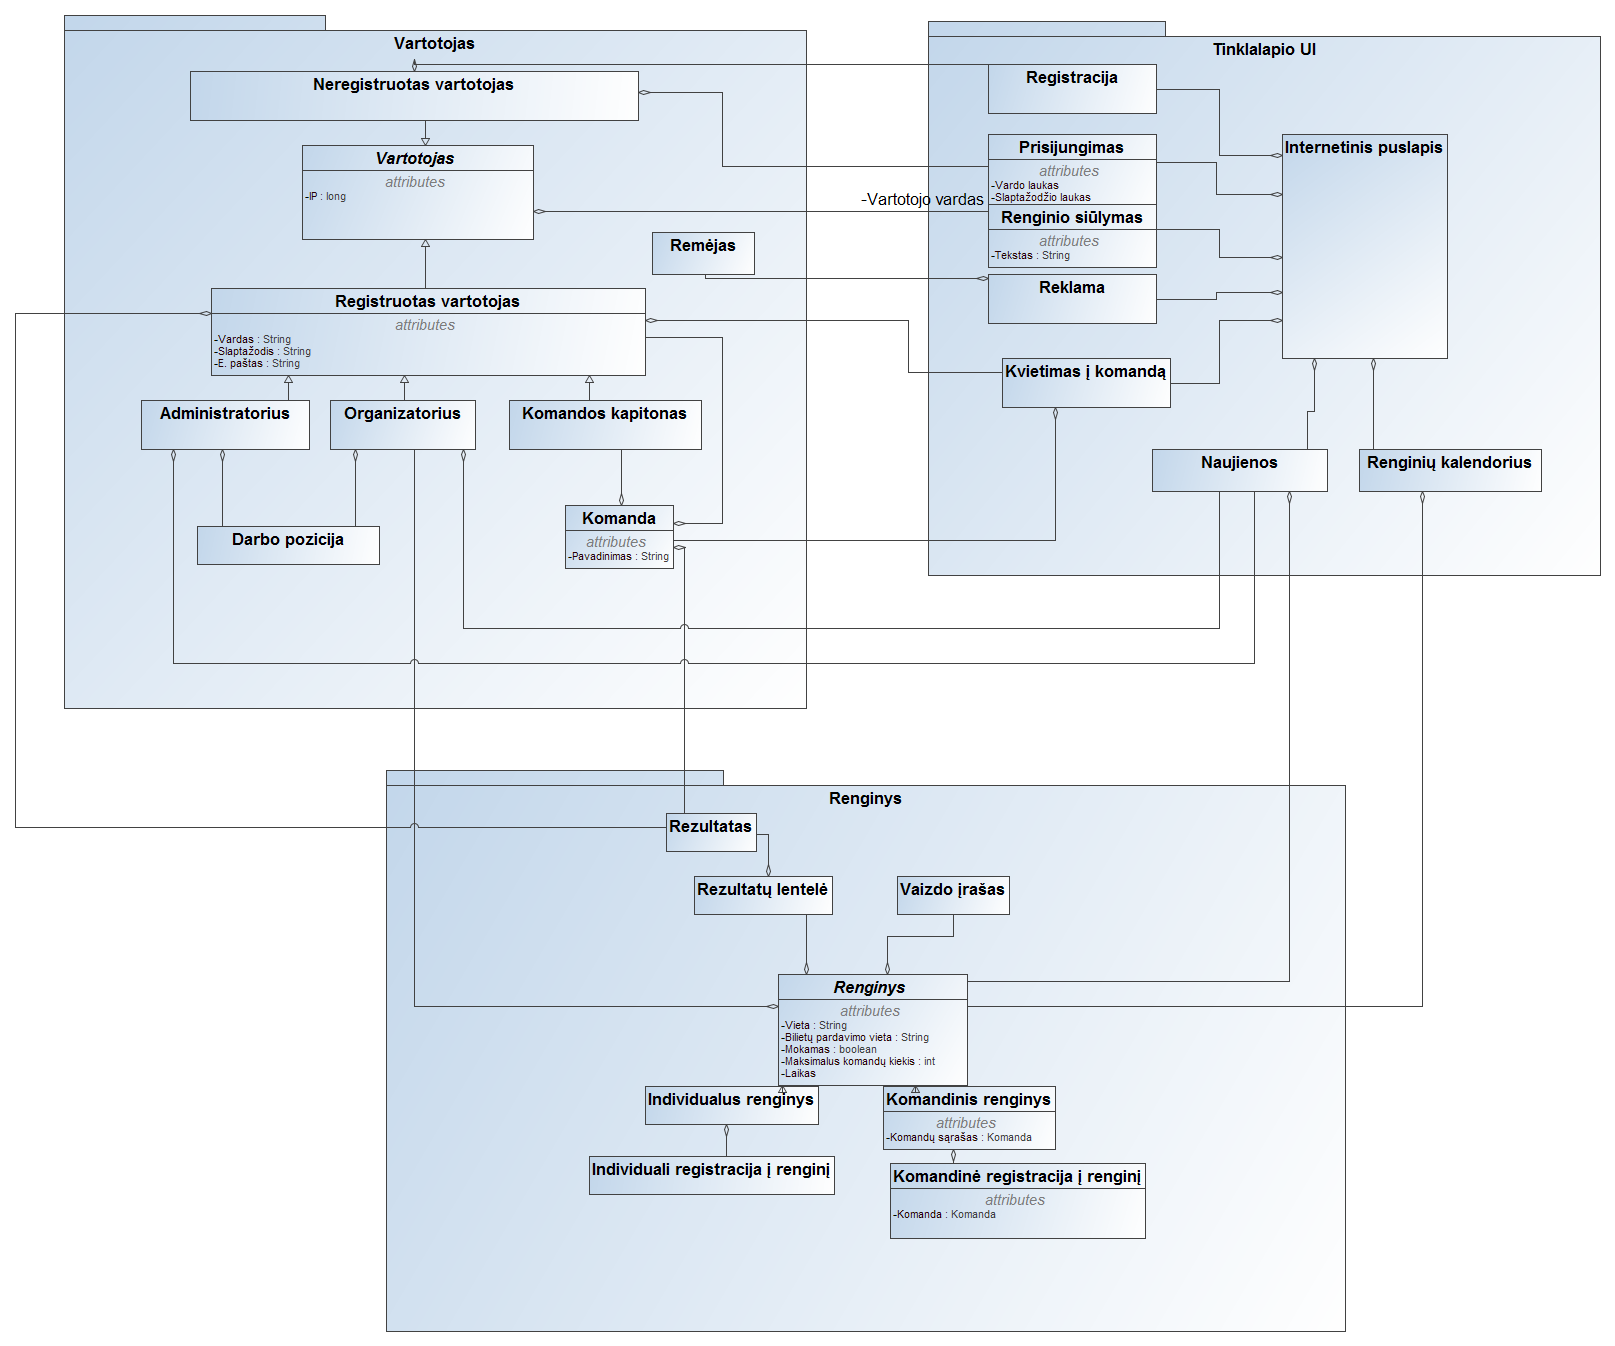
\includegraphics[width=\textwidth, height=20cm, keepaspectratio]{img/PSI4/Diagrams/ClassDiagram.png}
                \caption{Dalykinės srities modelio UML klasių diagrama}
                \label{fig:DS-klasiu-diagrama}
            \end{figure}
        \subsection*{Žodynas} \label{strukturinisDSModelis_zodynas}
            \begin{enumerate}[label=\textbf{E\arabic*.}]
					\item \textbf{Remėjas} - juridinis arba fizinis asmuo, skiriantis paramą tinklalapiui.
					\item \textbf{Registruotas vartotojas} - vartotojas, kurio duomenys (vartotojo vardas, slaptažodis) įrašyti į domenų bazę.
					\item \textbf{Prisijungęs vartotojas} - registruotas vartotojas, kuris tam tikru laiko momentų naudojasi tinklalapio paslaugomis.
					\item \textbf{Neprisijungęs vartotojas} - neautentifikuotas vartotojas, kuris tam tikru laiko momentu naudojasi tinklalapio paslaugomis.
					\item \textbf{Prisijungimas} -  registruoto, neprisijungusio vartotojo autentifikavimas pagal jo įvestą vartotojo vardą ir slaptažodį.
					\item \textbf{Naujiena} - administratoriaus arba renginio organizatorius paskelbtas skelbimas.
					\item \textbf{Renginių kalendorius} - renginių sąrašas, suskirstytas pagal renginių datą , atvaizduojamas lentelėje, rikuojamas pagal laiką.
					\item \textbf{Komandinis renginys} - sporto renginys, kuriame dalyvauja komandos.
					\item \textbf{Individualus renginys} - sporto renginys, kuriame dalyvauja individualūs asmenys.
					\item \textbf{Vaizdo įrašas} -  internete patalpintas vaizdo įrašas, rodomas per integruotą vaizdo įrašų grotuvą.
					\item \textbf{Registraciją į tinklalapį} - forma, į kurią neregistruotas vartotojas įveda vartotojo vardą || slaptažodį, vardą, pavardę, gimimo datą, telefono numerį, gyvenamoją vietą, elektroninio pašto adresą.
					\item \textbf{Individuali registracija į renginį} - mygtukas, leidžiantis patvirtinti prisijungusio vartotojo įtraukimą į renginio dalyvių sąrašą.
					\item \textbf{Komandinė registracija į renginį} -  formą, kurioje reikia nurodyti komandos pavadinimą ir registruotų vartotojų, kuriems bus siunčiami kvietimai, sąrašą.
					\item \textbf{Bilietas} - patvirtinimas, kad registruotas vartotojas turi teisę lankytis pasirinktame renginyje.
					\item \textbf{Darbo pozicija} - informacija apie neužimtą darbo poziciją renginio metu arba tinklalapio administracijoje.
					\item \textbf{Komanda} - registruotų vartotjų sąrašas, kurie priėmė kvietimus į komandą arba buvo priimti į komandą.
					\item \textbf{Kvietimas į komandą} - siūlymas prisijungti į komandą, kurį galima priimti arba atmesti.
					\item \textbf{Rezultatas} - asmens arba komandos, dalyvavusios renginyje, įvertinimas pagal tam tikrus kriterijus.
					\item \textbf{Rezultatų lentelė} - rezultatų sąrašas, atvaizduojamas lentelėje, filtruojamas ir rušiuojamas pagal pasirinktą kriterijų.
					\item \textbf{Renginio pasiūlymas} - prisijungusio arba neprisijungusio vartotojo atsiųstas renginio aprašymas, kurio administratorius dar nepublikavo.
					\item \textbf{Administratorius} - registruotas vartotojas, turintis teisę prisijungti prie administratoriaus skilties, peržiūrėti, pridėti, ištrinti, atnaujinti naujienas, renginius, renginio rezultatus ir vaizdo įrašus, apriboti, blokuoti vartotojus, peržiūrėti visų dalyvių, renginių, darbo aplikacijų sąrašus.
					\item \textbf{Organizatorius } - registruotas vartotojas, sukūręs arba norintis sistemoje sukurti renginį
					\item \textbf{Internetinis puslapis } - grafinė sistemos dalis, per kurią tekiamos sistemos paslaugos.
            \end{enumerate}
        \subsection{Reikalavimų - struktūrinio modelio atsekamumo matrica}\label{strukturinisDSModelis_matrica}
			\begin{table}[H]
				\centering
				\caption{Reikalavimų - struktūrinio modelio atsekamumo matrica}
				\label{ReikalavimųStruktūrinioModelioAtsekamumoMatrica}
				\begin{tabular}{|
				>{\columncolor[HTML]{9B9B9B}}l|l|l|l|l|l|l|l|l|l|l|l|l|l|l|l|l|l|l|l|l|l|} \hline X & 
				\cellcolor[HTML]{D3D3D3}\rotatebox[origin=c]{90}{FR1} & \cellcolor[HTML]{9B9B9B}\rotatebox[origin=c]{90}{FR2} &
				\cellcolor[HTML]{9B9B9B}\rotatebox[origin=c]{90}{FR3} & \cellcolor[HTML]{9B9B9B}\rotatebox[origin=c]{90}{FR4} & 
				\cellcolor[HTML]{9B9B9B}\rotatebox[origin=c]{90}{FR5} & \cellcolor[HTML]{9B9B9B}\rotatebox[origin=c]{90}{FR6} & 
				\cellcolor[HTML]{9B9B9B}\rotatebox[origin=c]{90}{FR7} & \cellcolor[HTML]{9B9B9B}\rotatebox[origin=c]{90}{FR8} & 
				\cellcolor[HTML]{9B9B9B}\rotatebox[origin=c]{90}{FR9} & \cellcolor[HTML]{9B9B9B}\rotatebox[origin=c]{90}{FR10} & 
				\cellcolor[HTML]{9B9B9B}\rotatebox[origin=c]{90}{FR11} & \cellcolor[HTML]{9B9B9B}\rotatebox[origin=c]{90}{FR12} & 
				\cellcolor[HTML]{9B9B9B}\rotatebox[origin=c]{90}{FR13} & \cellcolor[HTML]{9B9B9B}\rotatebox[origin=c]{90}{FR14} & 
				\cellcolor[HTML]{9B9B9B}\rotatebox[origin=c]{90}{FR15} & \cellcolor[HTML]{9B9B9B}\rotatebox[origin=c]{90}{FR16} &
				\cellcolor[HTML]{9B9B9B}\rotatebox[origin=c]{90}{FR17} & \cellcolor[HTML]{9B9B9B}\rotatebox[origin=c]{90}{FR18} & 
				\cellcolor[HTML]{9B9B9B}\rotatebox[origin=c]{90}{FR19} & \cellcolor[HTML]{9B9B9B}\rotatebox[origin=c]{90}{FR20} &
				\cellcolor[HTML]{9B9B9B}\rotatebox[origin=c]{90}{FR21} \\ \hline
				E1  &      &      &      &      &      &      &      &      &      &      &      &      &      &      &      & X    &      &      &      &      &      \\ \hline
				E2  & X    &      &      & X    &      &      & X    &      &      &      &      &      & X    &      &      &      &      &      &      &      &      \\ \hline
				E3  &      &      & X    &      &      &      &      &      &      &      &      &      &      &      & X    &      &      &      &      &      &      \\ \hline
				E4  & X    & X    &      &      &      &      &      &      &      &      &      &      &      &      &      &      &      &      &      &      &      \\ \hline
				E5  &      & X    &      &      &      &      &      &      &      &      &      &      &      &      &      &      &      &      &      &      &      \\ \hline
				E6  &      & X    &      &      &      &      &      &      &      &      &      &      &      &      &      &      &      & X    &      &      &      \\ \hline
				E7  &      & X    &      &      &      &      &      &      &      &      &      &      &      &      &      &      &      &      &      &      &      \\ \hline
				E8  &      &      &      &      &      &      &      &      &      & X    &      &      &      &      &      &      &      & X    &      &      &      \\ \hline
				E9  &      &      &      &      &      &      &      &      &      & X    &      &      &      &      &      &      &      & X    &      &      &      \\ \hline
				E10 &      & X    & X    &      &      &      &      &      & X    &      &      &      &      &      &      &      &      & X    &      &      &      \\ \hline
				E11 &      &      &      & X    &      &      &      &      &      &      &      &      &      &      &      &      &      &      &      &      &      \\ \hline
				E12 &      &      &      &      & X    &      &      &      &      &      &      &      &      &      &      &      &      &      &      &      &      \\ \hline
				E13 &      &      &      &      & X    & X    &      &      &      &      &      &      &      &      &      &      &      &      &      &      &      \\ \hline
				E14 &      &      &      &      &      &      &      &      &      &      &      &      &      &      &      &      &      &      & X    &      &      \\ \hline
				E15 &      &      &      &      & X    &      &      &      &      &      &      &      &      &      &      &      &      &      &      &      &      \\ \hline
				E16 &      &      &      &      &      & X    & X    &      &      &      &      &      & X    &      &      &      &      &      &      &      &      \\ \hline
				E17 &      &      &      &      &      &      & X    & X    &      &      &      &      &      &      &      &      &      &      &      &      &      \\ \hline
				E18 &      &      &      &      &      &      &      &      &      &      & X    &      & X    &      &      &      &      & X    &      &      &      \\ \hline
				E19 &      &      &      &      &      &      &      &      &      & X    & X    & X    &      &      &      &      &      &      &      &      &      \\ \hline
				E20 &      & X    &      &      &      &      &      &      &      &      &      &      &      & X    & X    &      &      &      &      &      &      \\ \hline
				E21 &      &      &      &      &      &      &      &      &      &      &      &      &      &      &      &      & X    & X    &      &      &      \\ \hline
				E22 &      &      &      &      &      &      &      &      &      &      &      &      &      & X    &      &      &      &      &      &      &      \\ \hline
				E23 &      &      &      &      &      &      &      &      &      &      &      &      &      &      &      &      &      &      &      & X    & X    \\ \hline
				\end{tabular}
			\end{table} 
			
    \section{Užduotys}\label{uzduotys}
		Šiame skyriuje pateikiamos pagrindinės neprisijungusio, prisijungusio ir paprasto vartotojo, komandos vadovo, administratoriaus ir organizatoriaus užduotys.
		Taip pat pateikiama bendra UML diagrama apibrėžianti visų šių agentų užduotis.
			\noindent
			
			\begin{figure}[H]
                \centering
                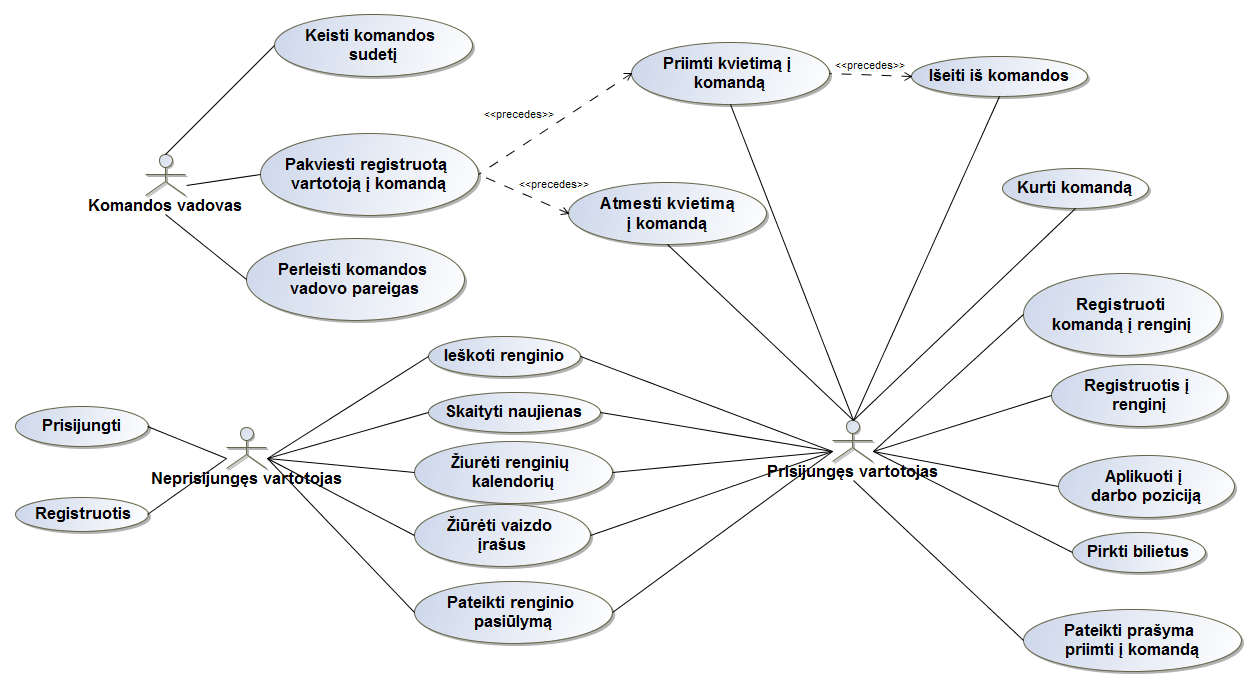
\includegraphics[width=\textwidth]{img/PSI4/Diagrams/UCuser.png}
                \caption{UML neprisijungusių, prisijungusių vartotojų ir komandos vadovo užduočių diagrama}
                \label{fig:uzduociu-diagrama}
            \end{figure}
			
			\begin{figure}[H]
                \centering
                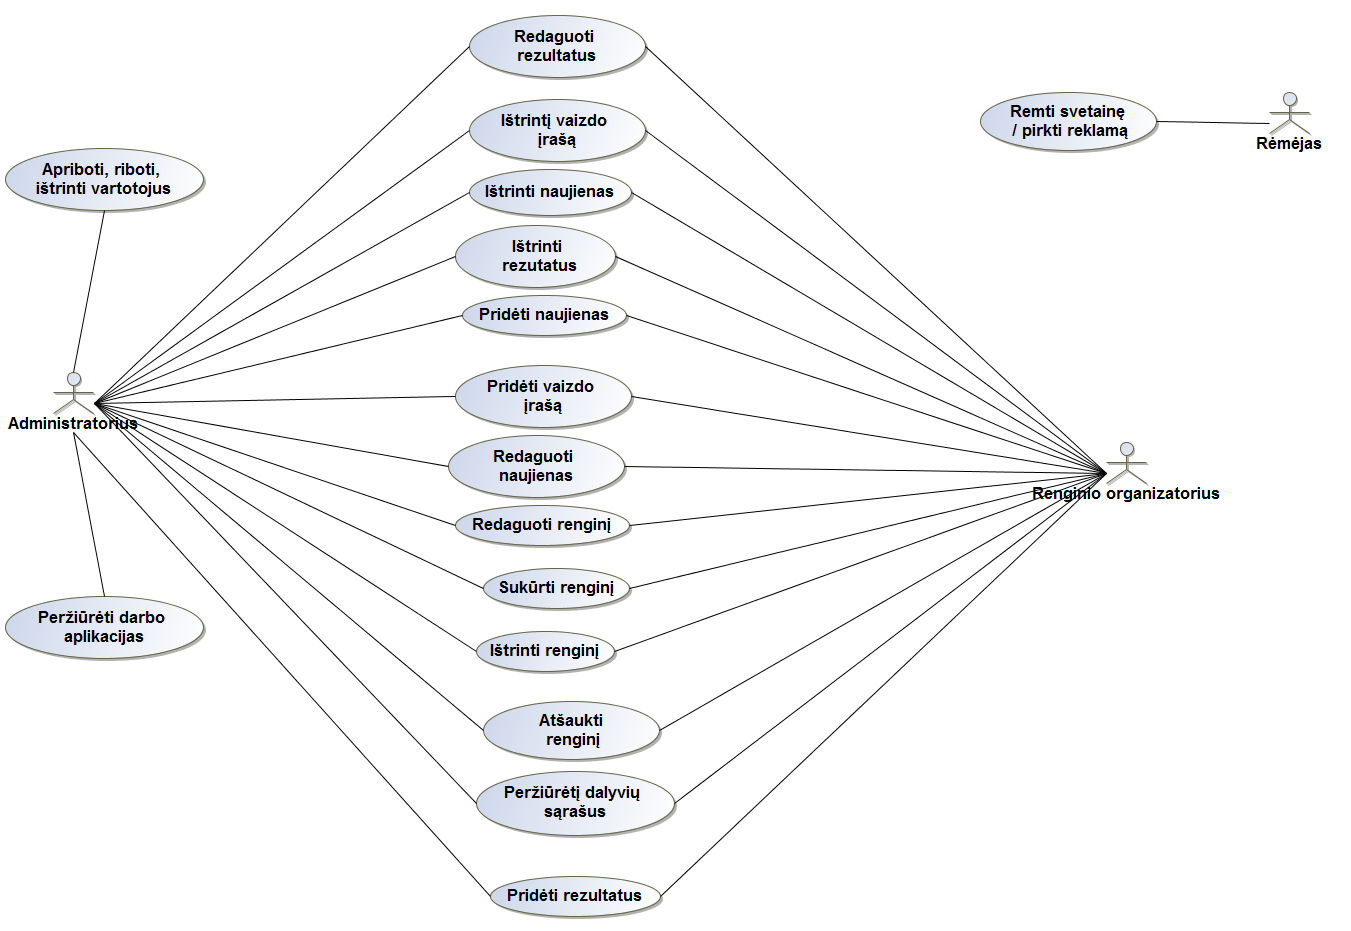
\includegraphics[width=\textwidth]{img/PSI4/Diagrams/UCadmin.png}
                \caption{UML administratoriaus, organizatoriaus ir rėmėjo užduočių diagrama}
                \label{fig:uzduociu-diagrama2}
            \end{figure}
		\newpage
		\begin{enumerate} [label = \textbf{U\arabic*.}]
			\item \textbf{Skaityti naujienas} \\
				Vartotojas paspaudžia ant mygtuko ,,Naujienos'', kuris yra navigacijos meniu. Tada vartotojas yra nukeliamas yra puslapį ,,Naujienos'', kuriame yra naujienų trupi aprašymai. Vartotojas paspaudžia ant naujienos, atidaromas visas naujienos tekstas.
				
				\underline{Alternatyvūs scenarijai:}
				\begin{itemize}
					\item Jei naujienų nėra, vartotojas paspaudęs ant mygtuko ,,Naujienos'' yra nukeliamas į puslapį ,,Naujienos'', kuriame nėra straipsnių, bet yra užrašas ,,Atsiprašome, šiuo metu straipsnių neturime''. 
				\end{itemize}

				\begin{figure}[H]
					\centering
					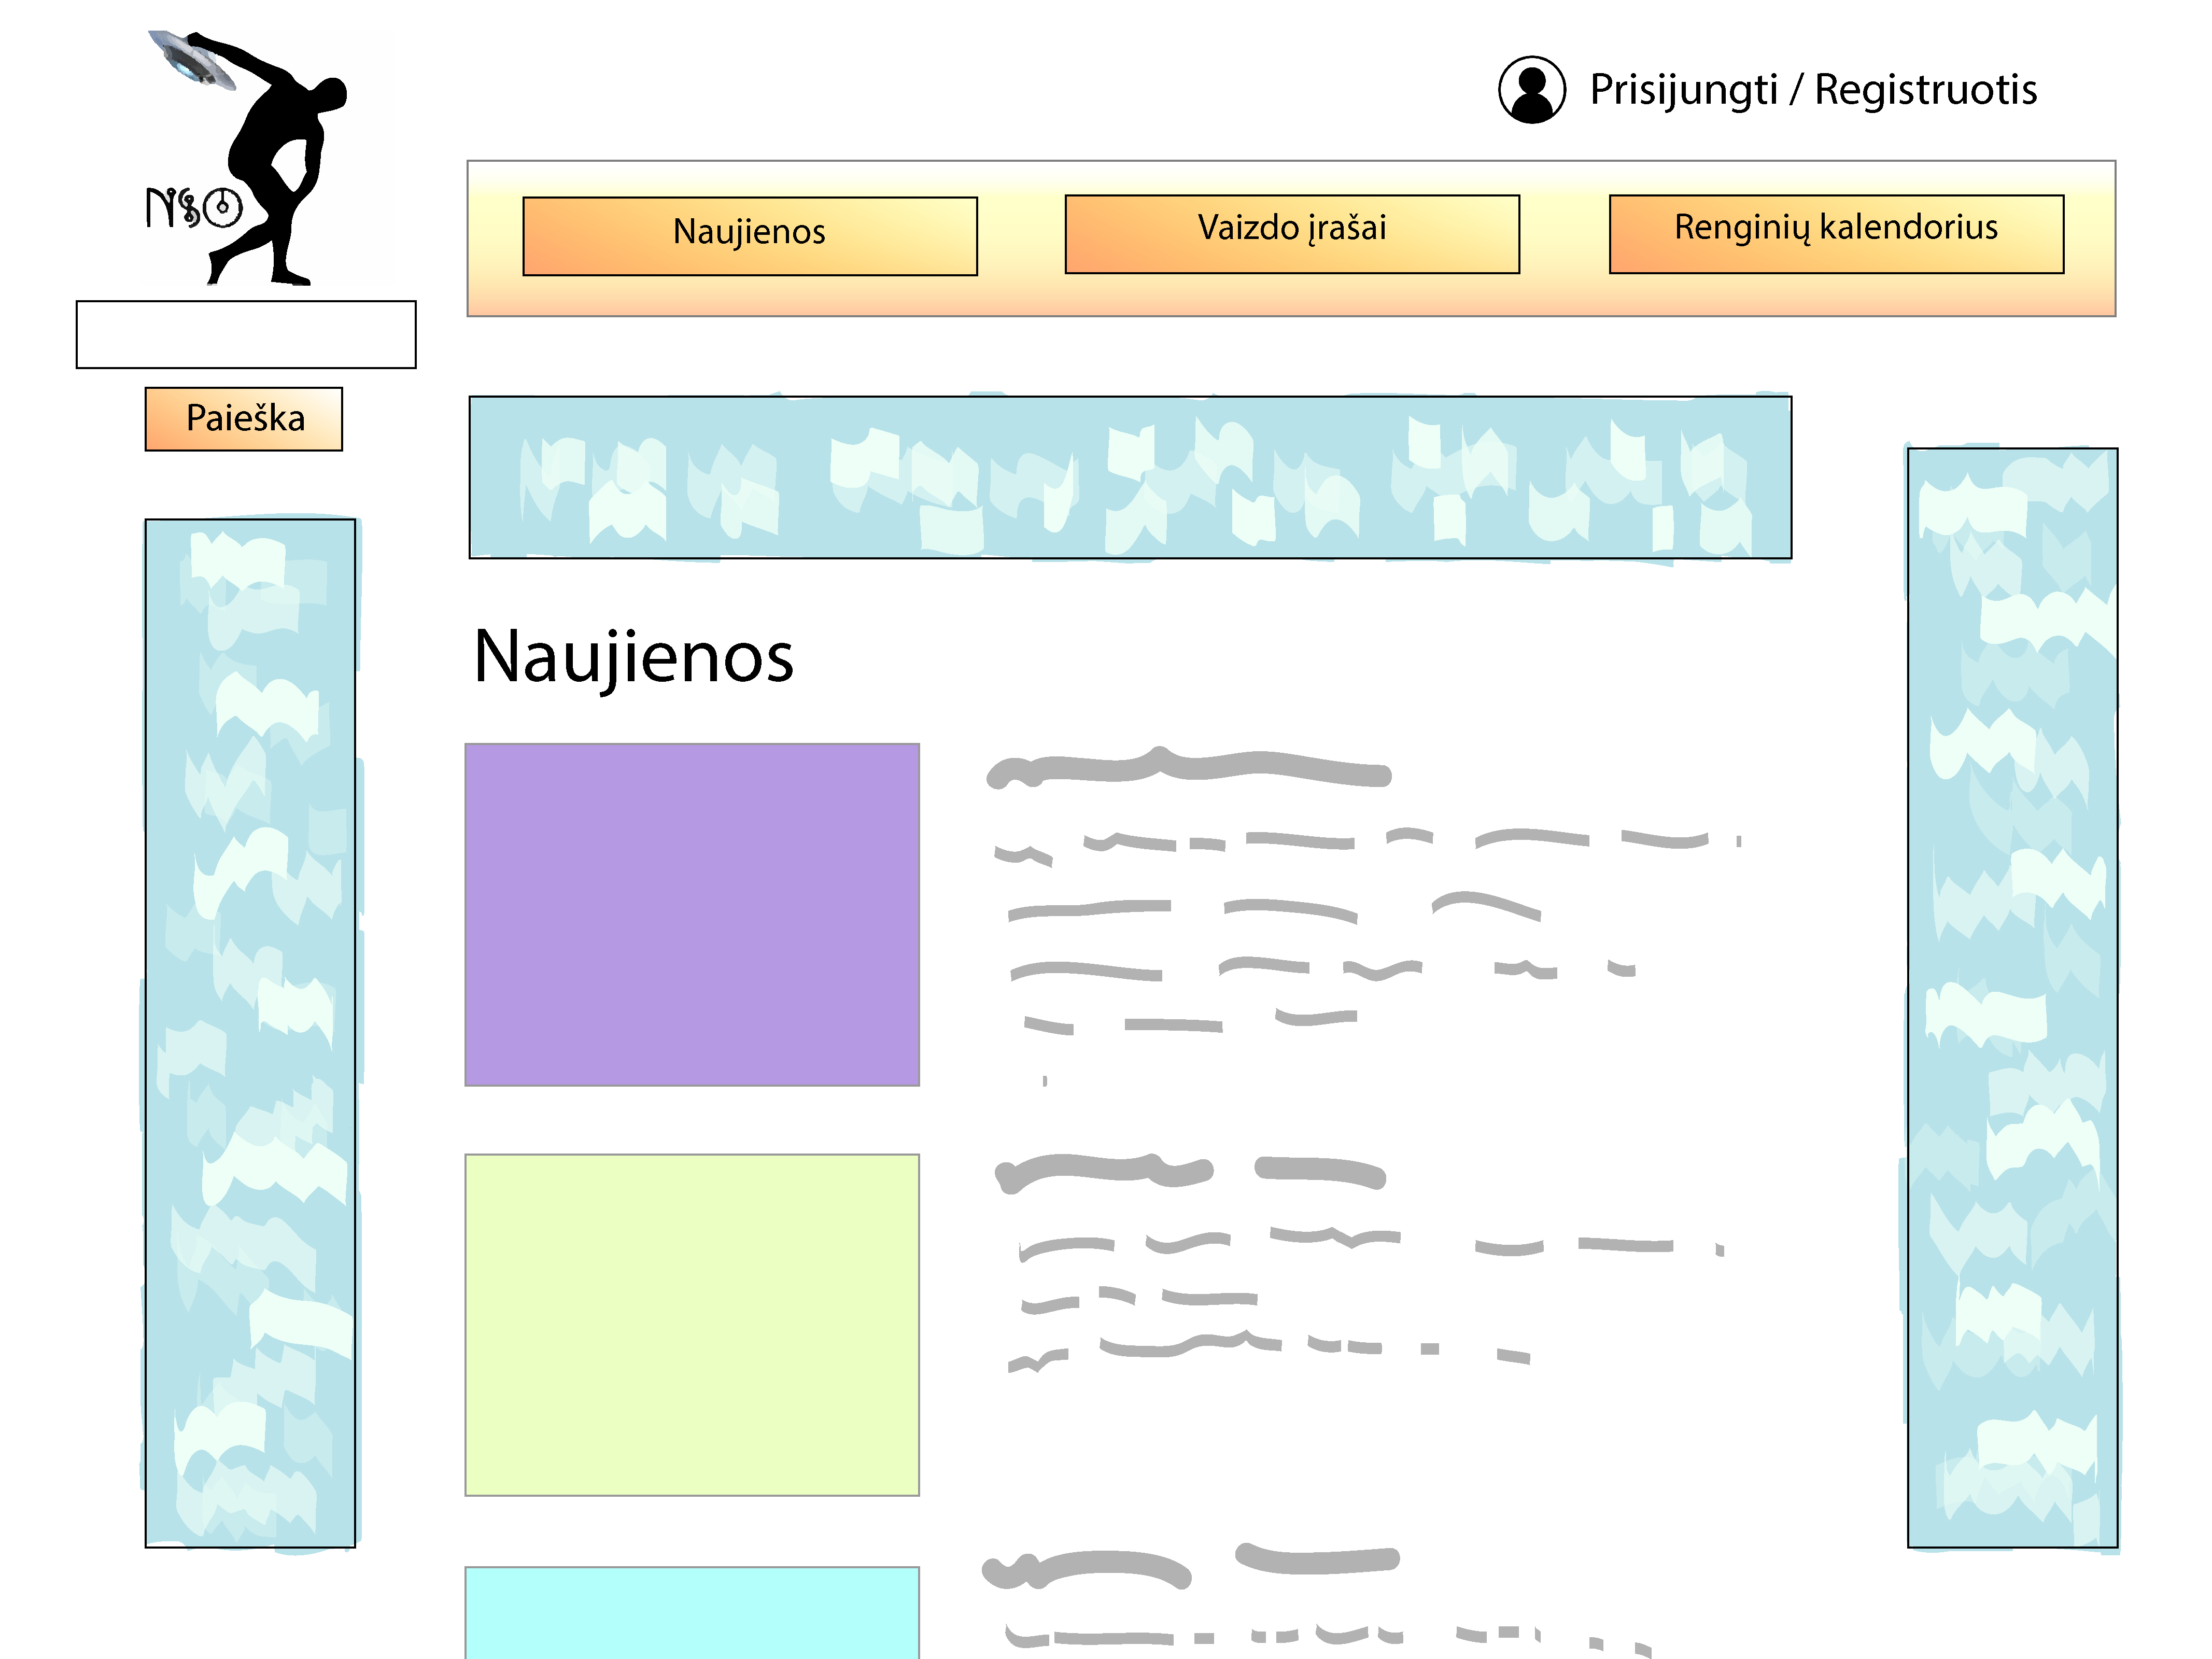
\includegraphics[width=\textwidth, height=11cm, keepaspectratio]{img/PSI4/Naujienos-01.jpg}
					\caption{Naujienų skaitymas}
					\label{fig:uzd_skaitymas}
				\end{figure}
				
			\item \textbf{Žiūrėti renginių kalendorių} \\
				Vartotojas spaudžia ant mygtuko ,,Renginių kalendorius'', kuris yra navigacijos meniu. Tada vartotojas yra nukeliamas į puslapį ,,Renginių kalendorius'', kuriame peržiūri renginius sudėtus pagal jų datas į atitinkamas kalendoriaus dienas, turint galimybę keisti mėnesius.
				
				\underline{Alternatyvūs scenarijai:}
				\begin{itemize}
					\item Vartotojas nemato visų renginių vykstančių tą pačią dieną, nes jų vyksta per daug. Tada kalendoriaus dienos langelis talpina kelis renginius ir tritaškio paveiksliuką, ant kurio paspaudus atidaromas naujas puslapis su sąrašu renginių vykstančių tą dieną.
					\item Vartotojui, norint daugiau informacijos apie renginį, paspaudžia ant renginio pavadinimo ir yra atidaromas kitas puslapis su renginio informacija.
				\end{itemize}
				
				\begin{figure}[H]
						\centering
						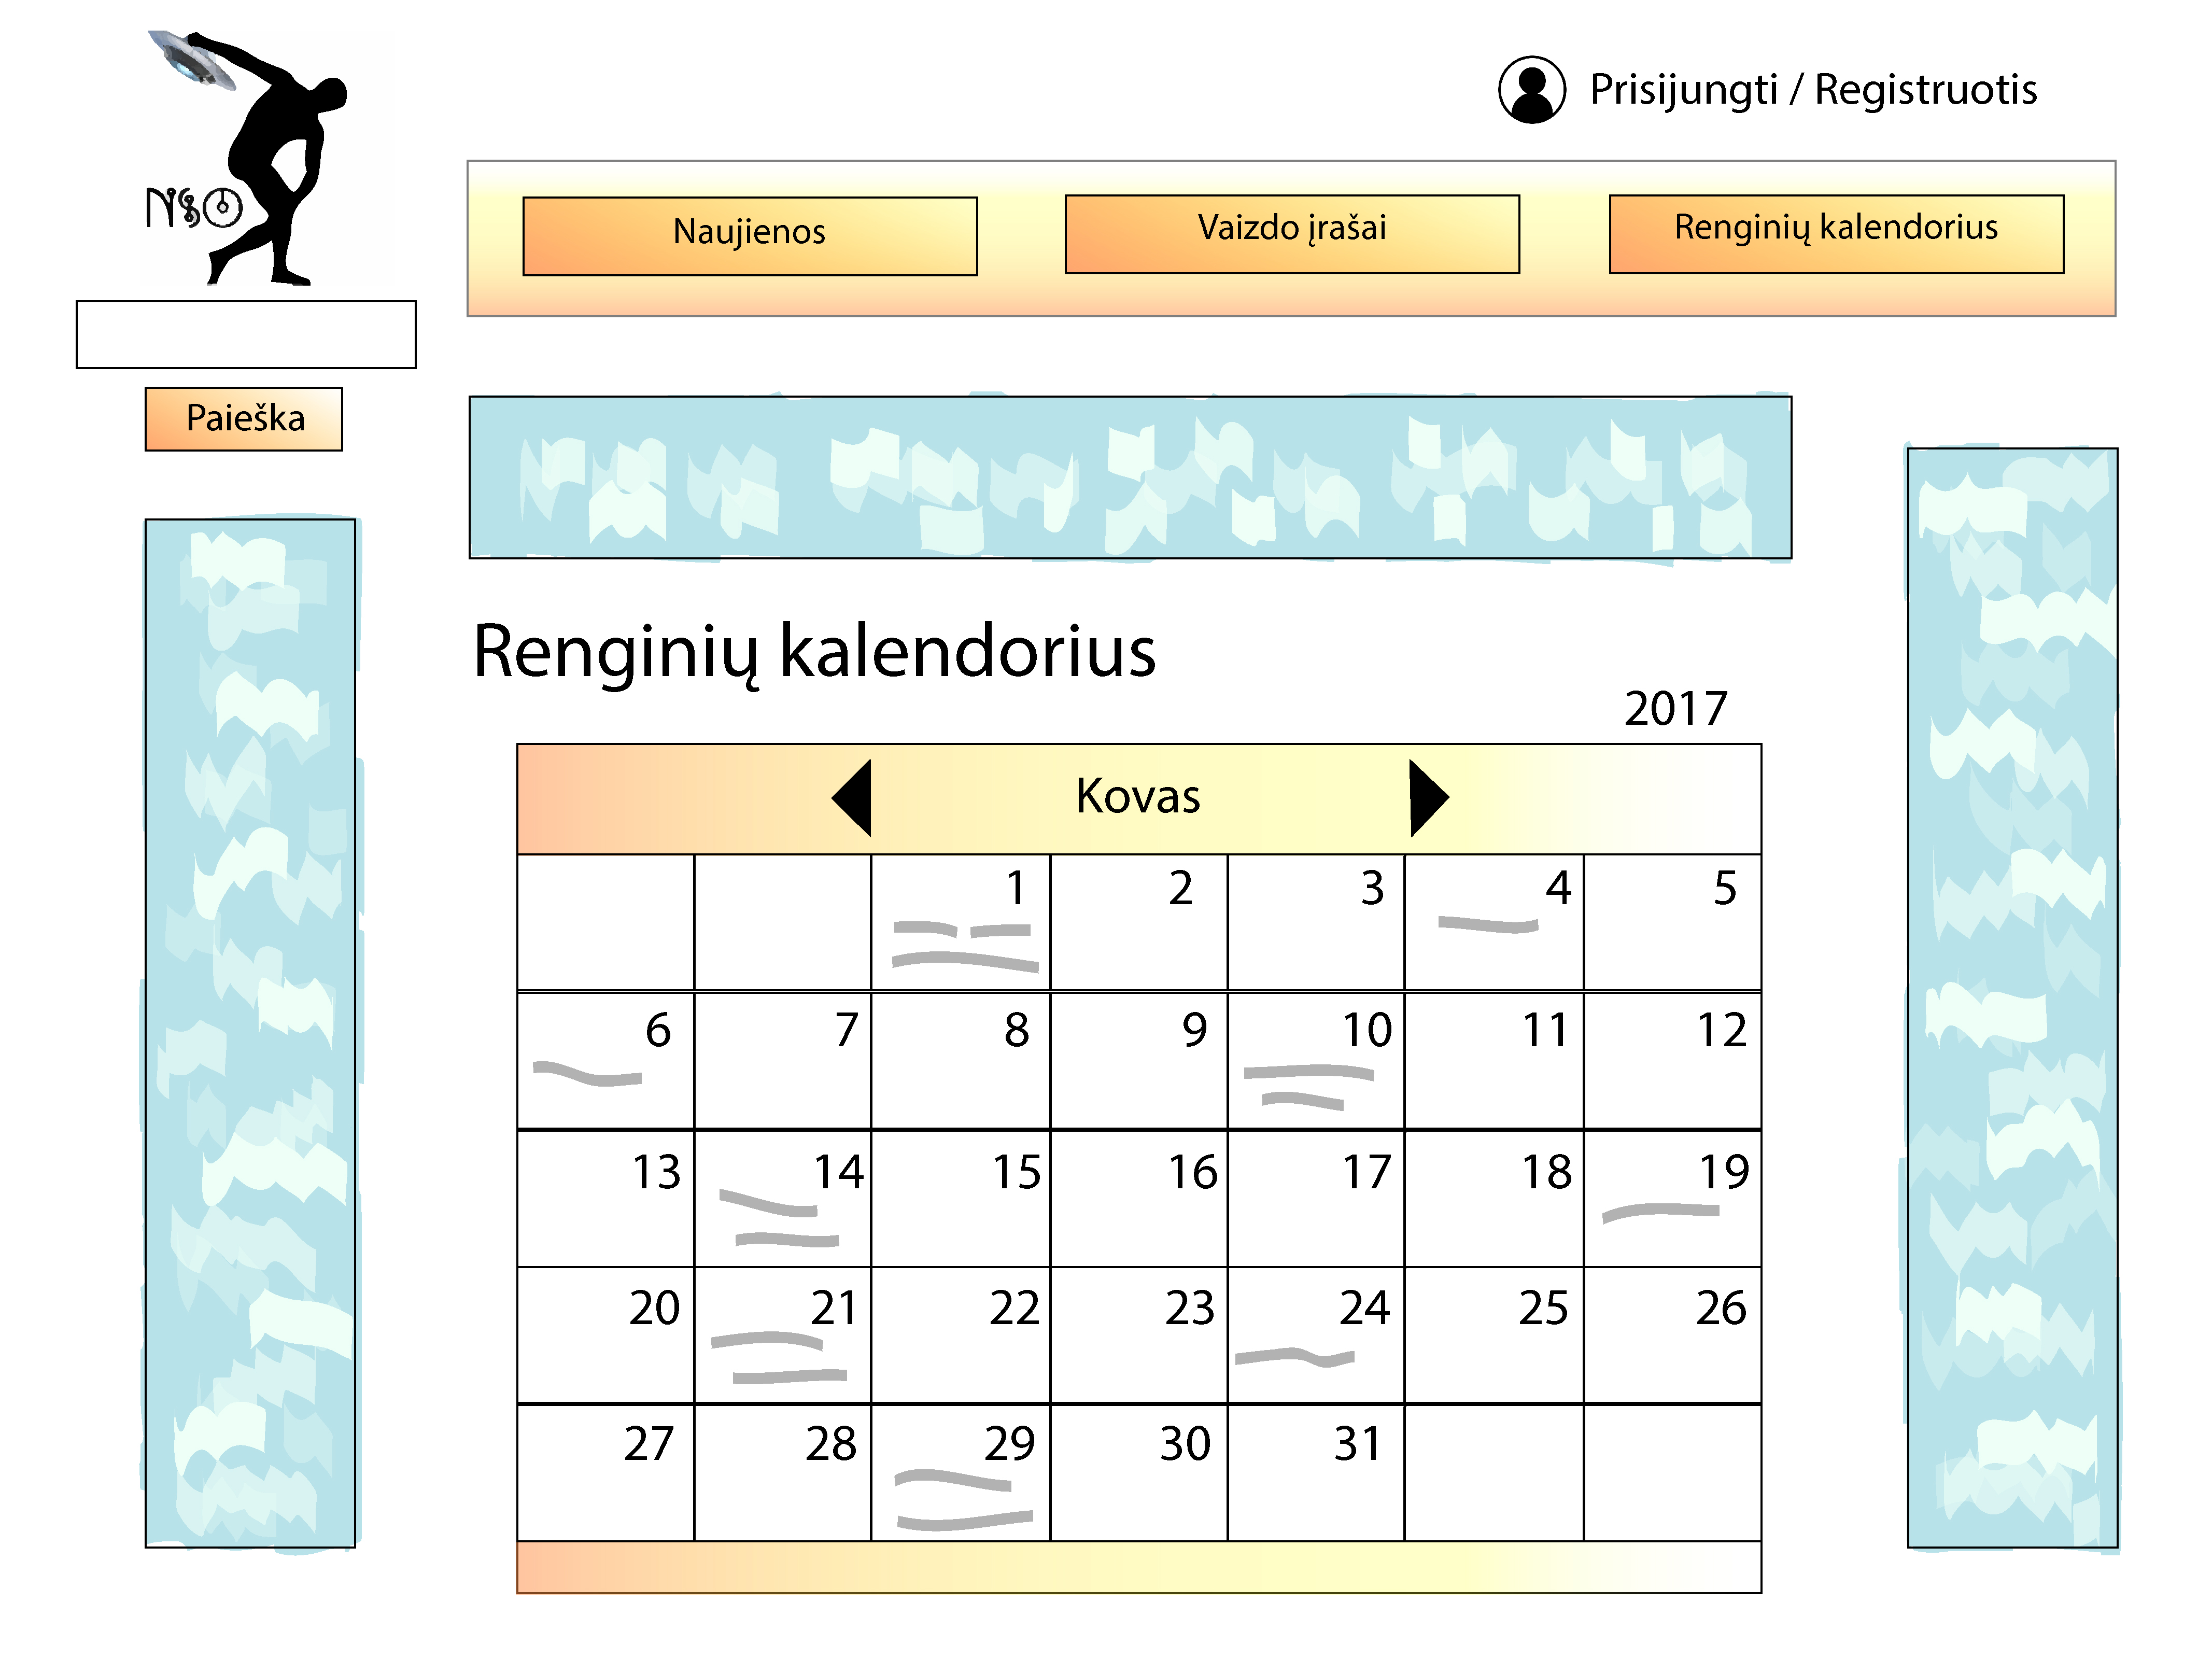
\includegraphics[width=\textwidth, height=5cm, keepaspectratio]{img/PSI4/RenginioKalendorius-01.jpg}
						\caption{Renginio kalendorius}
						\label{fig:uzd_reginioKalendorius}
					\end{figure}

			\item \textbf{Ieškoti renginio} \\
					Vartotojas paieškos laukelyje įveda paieškos žodį ir tada yra atidaromas naujas puslapis, kuriame yra visi renginiai turintys paieškos žodį.
					
				\underline{Alternatyvūs scenarijai:}
				\begin{itemize}
						\item Vartotojas suveda paieškos žodį, kuris neturi jokio atitikmens renginių pavadinime ar informacijoje apie juos. Tada atidaromas naujas puslapis, kuriame parašyta ,,Atsiprašome, nieko su paieškos žodžiu neradome.'' 
				\end{itemize}

				\begin{figure}[H]
					\centering
					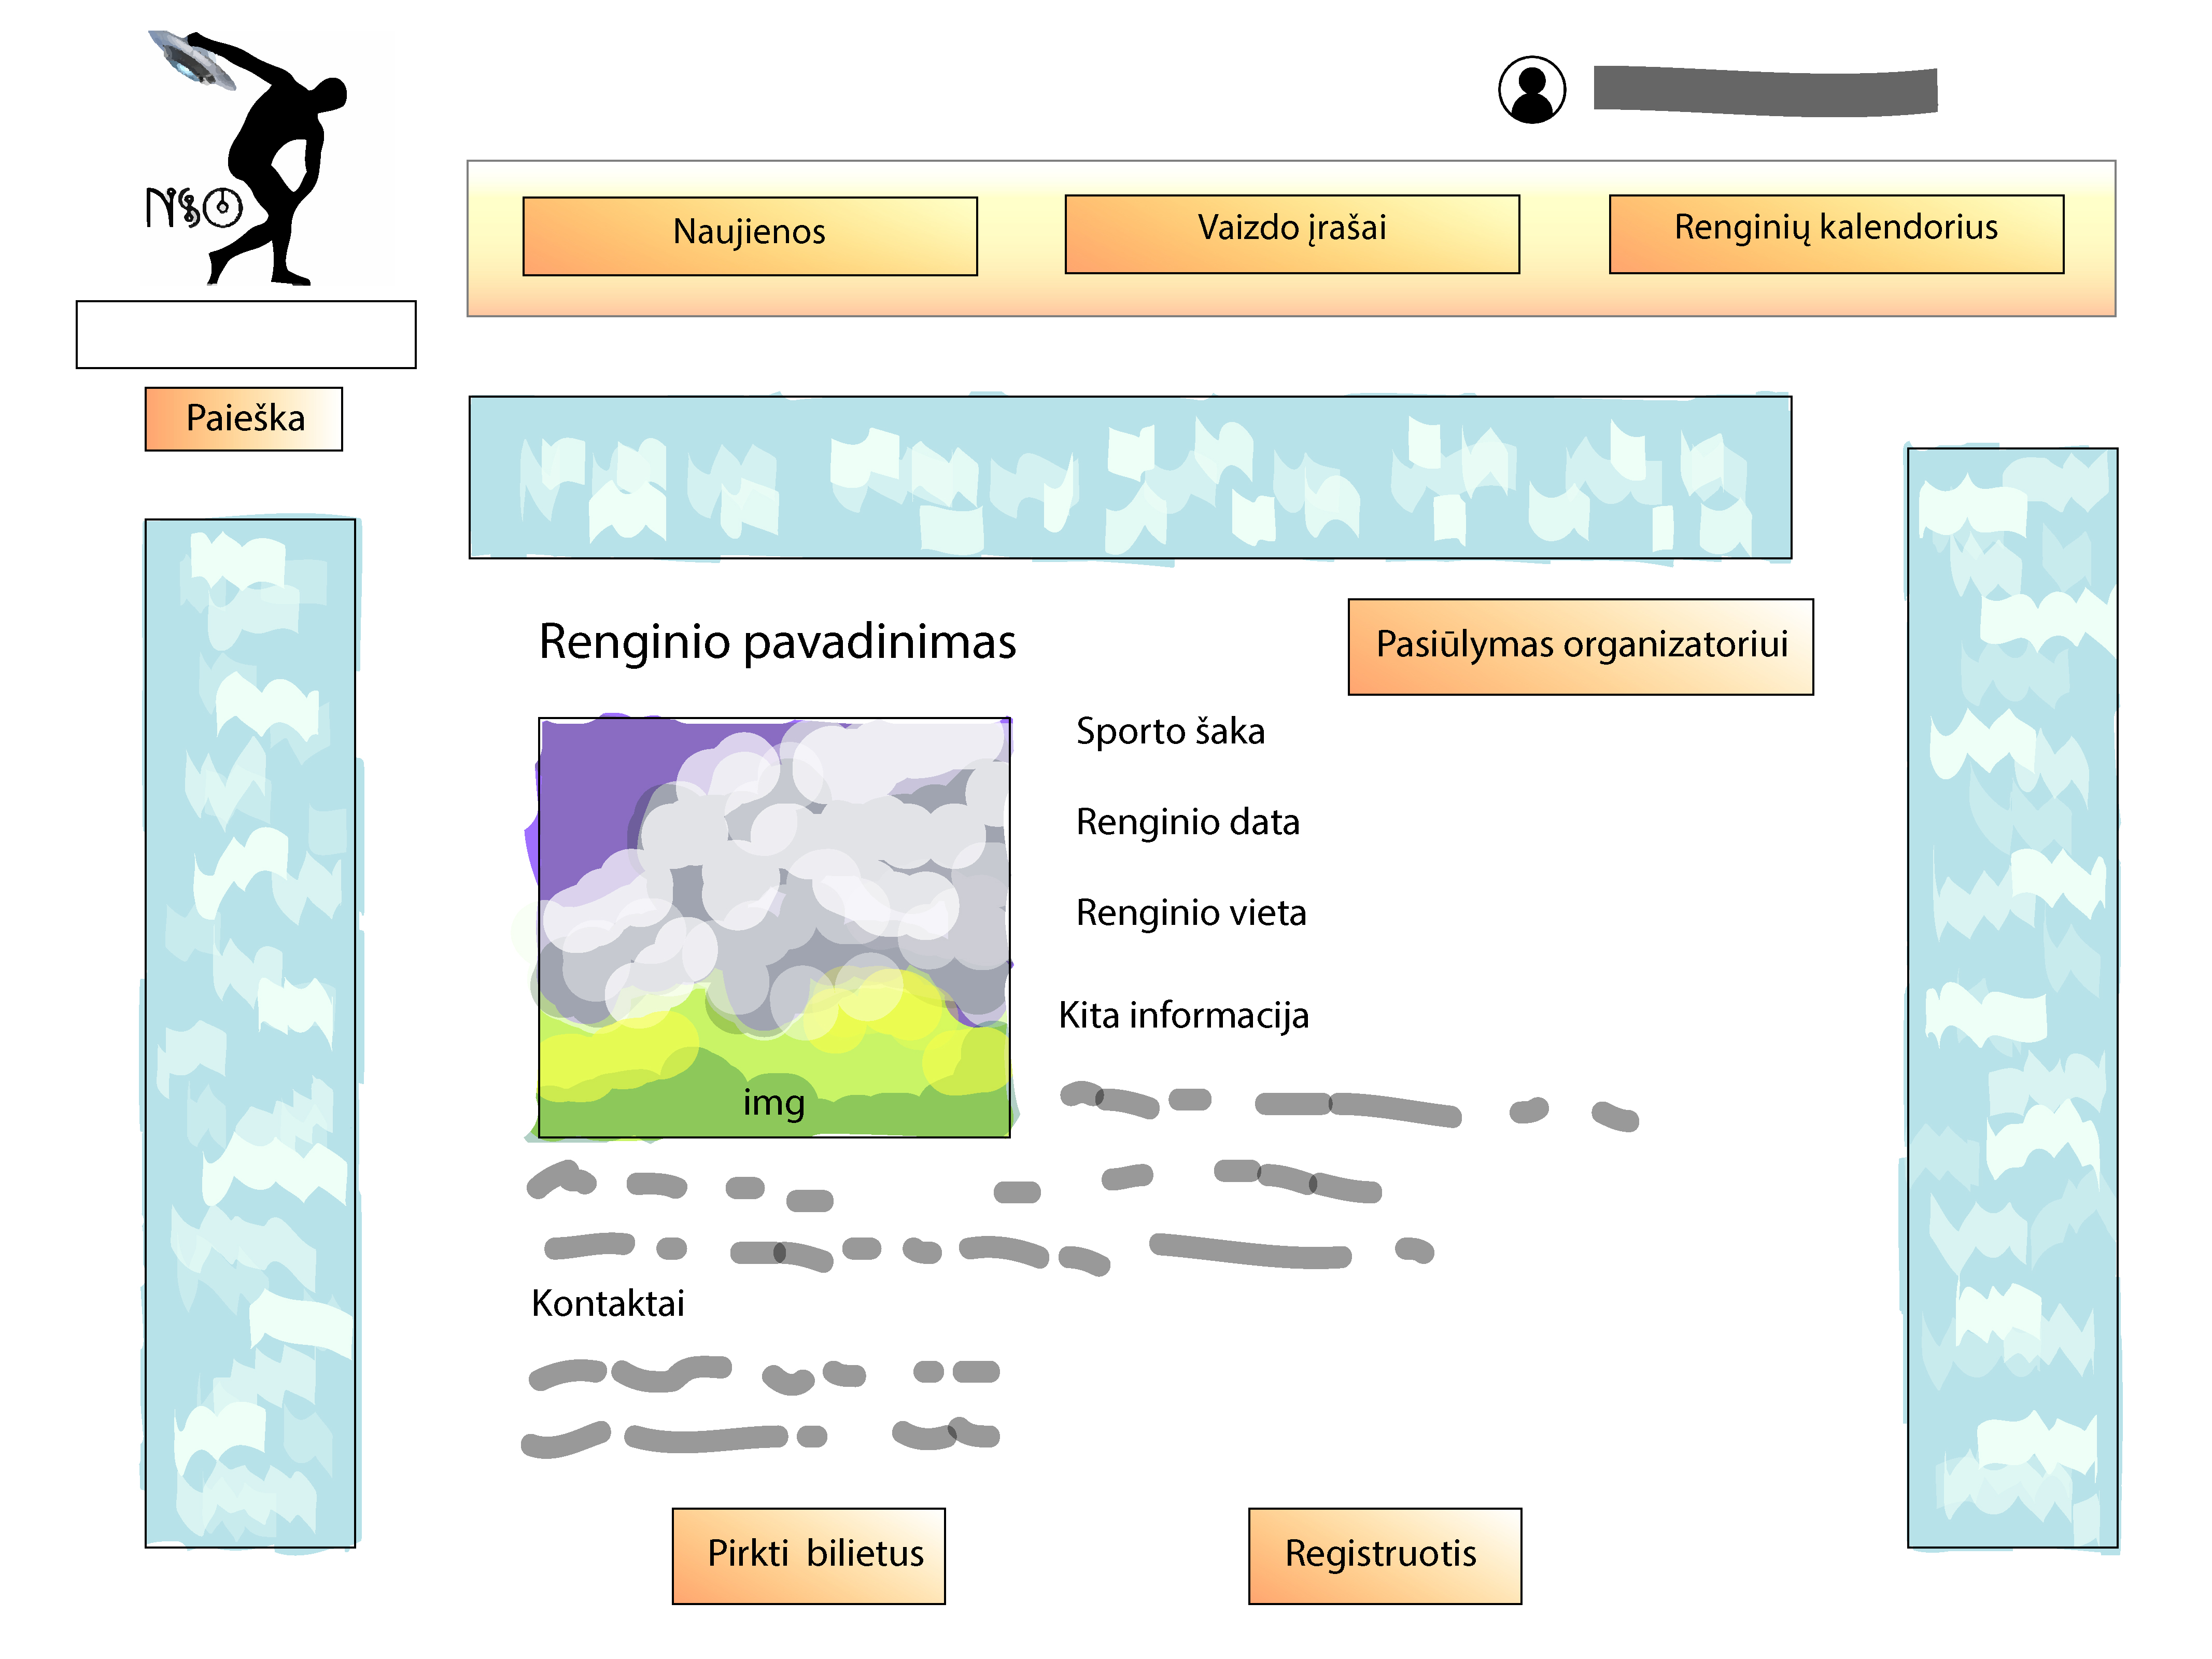
\includegraphics[width=\textwidth]{img/PSI4/renginioPuslapis-01.jpg}
					\caption{Renginio puslapis}
					\label{fig:uzd_renginiai}
				\end{figure}
				
			\item \textbf{Žiūrėti vaizdo įrašus} \\
				Vartotojas spaudžia ant mygtuko ,,Vaizdo įrašai'' ir tada jis yra nukeliamas į puslapį ,,Vaizdo įrašai''. Jame vartotojas pasirenka iš vaizdo įrašų sąrašo, kurį nori žiūrėti. Pasirinkęs vaizdo įrašą paspaudžia ant jo. Vaizdo įrašas iškylą per visą ekraną ir pasileidžia.
				
				\underline{Alternatyvūs scenarijai:}
				\begin{itemize}
					\item Vartotojui neturinčiam ,,Adobe Flash Player'' ir paspaudus ant vaizdo įrašo yra išmetamas pranešimas - ,,Jūs neturite ,,Adobe Flash Player'' todėl video negalėsite pasižiūrėti''.
				\end{itemize}

				\begin{figure}[H]
					\centering
					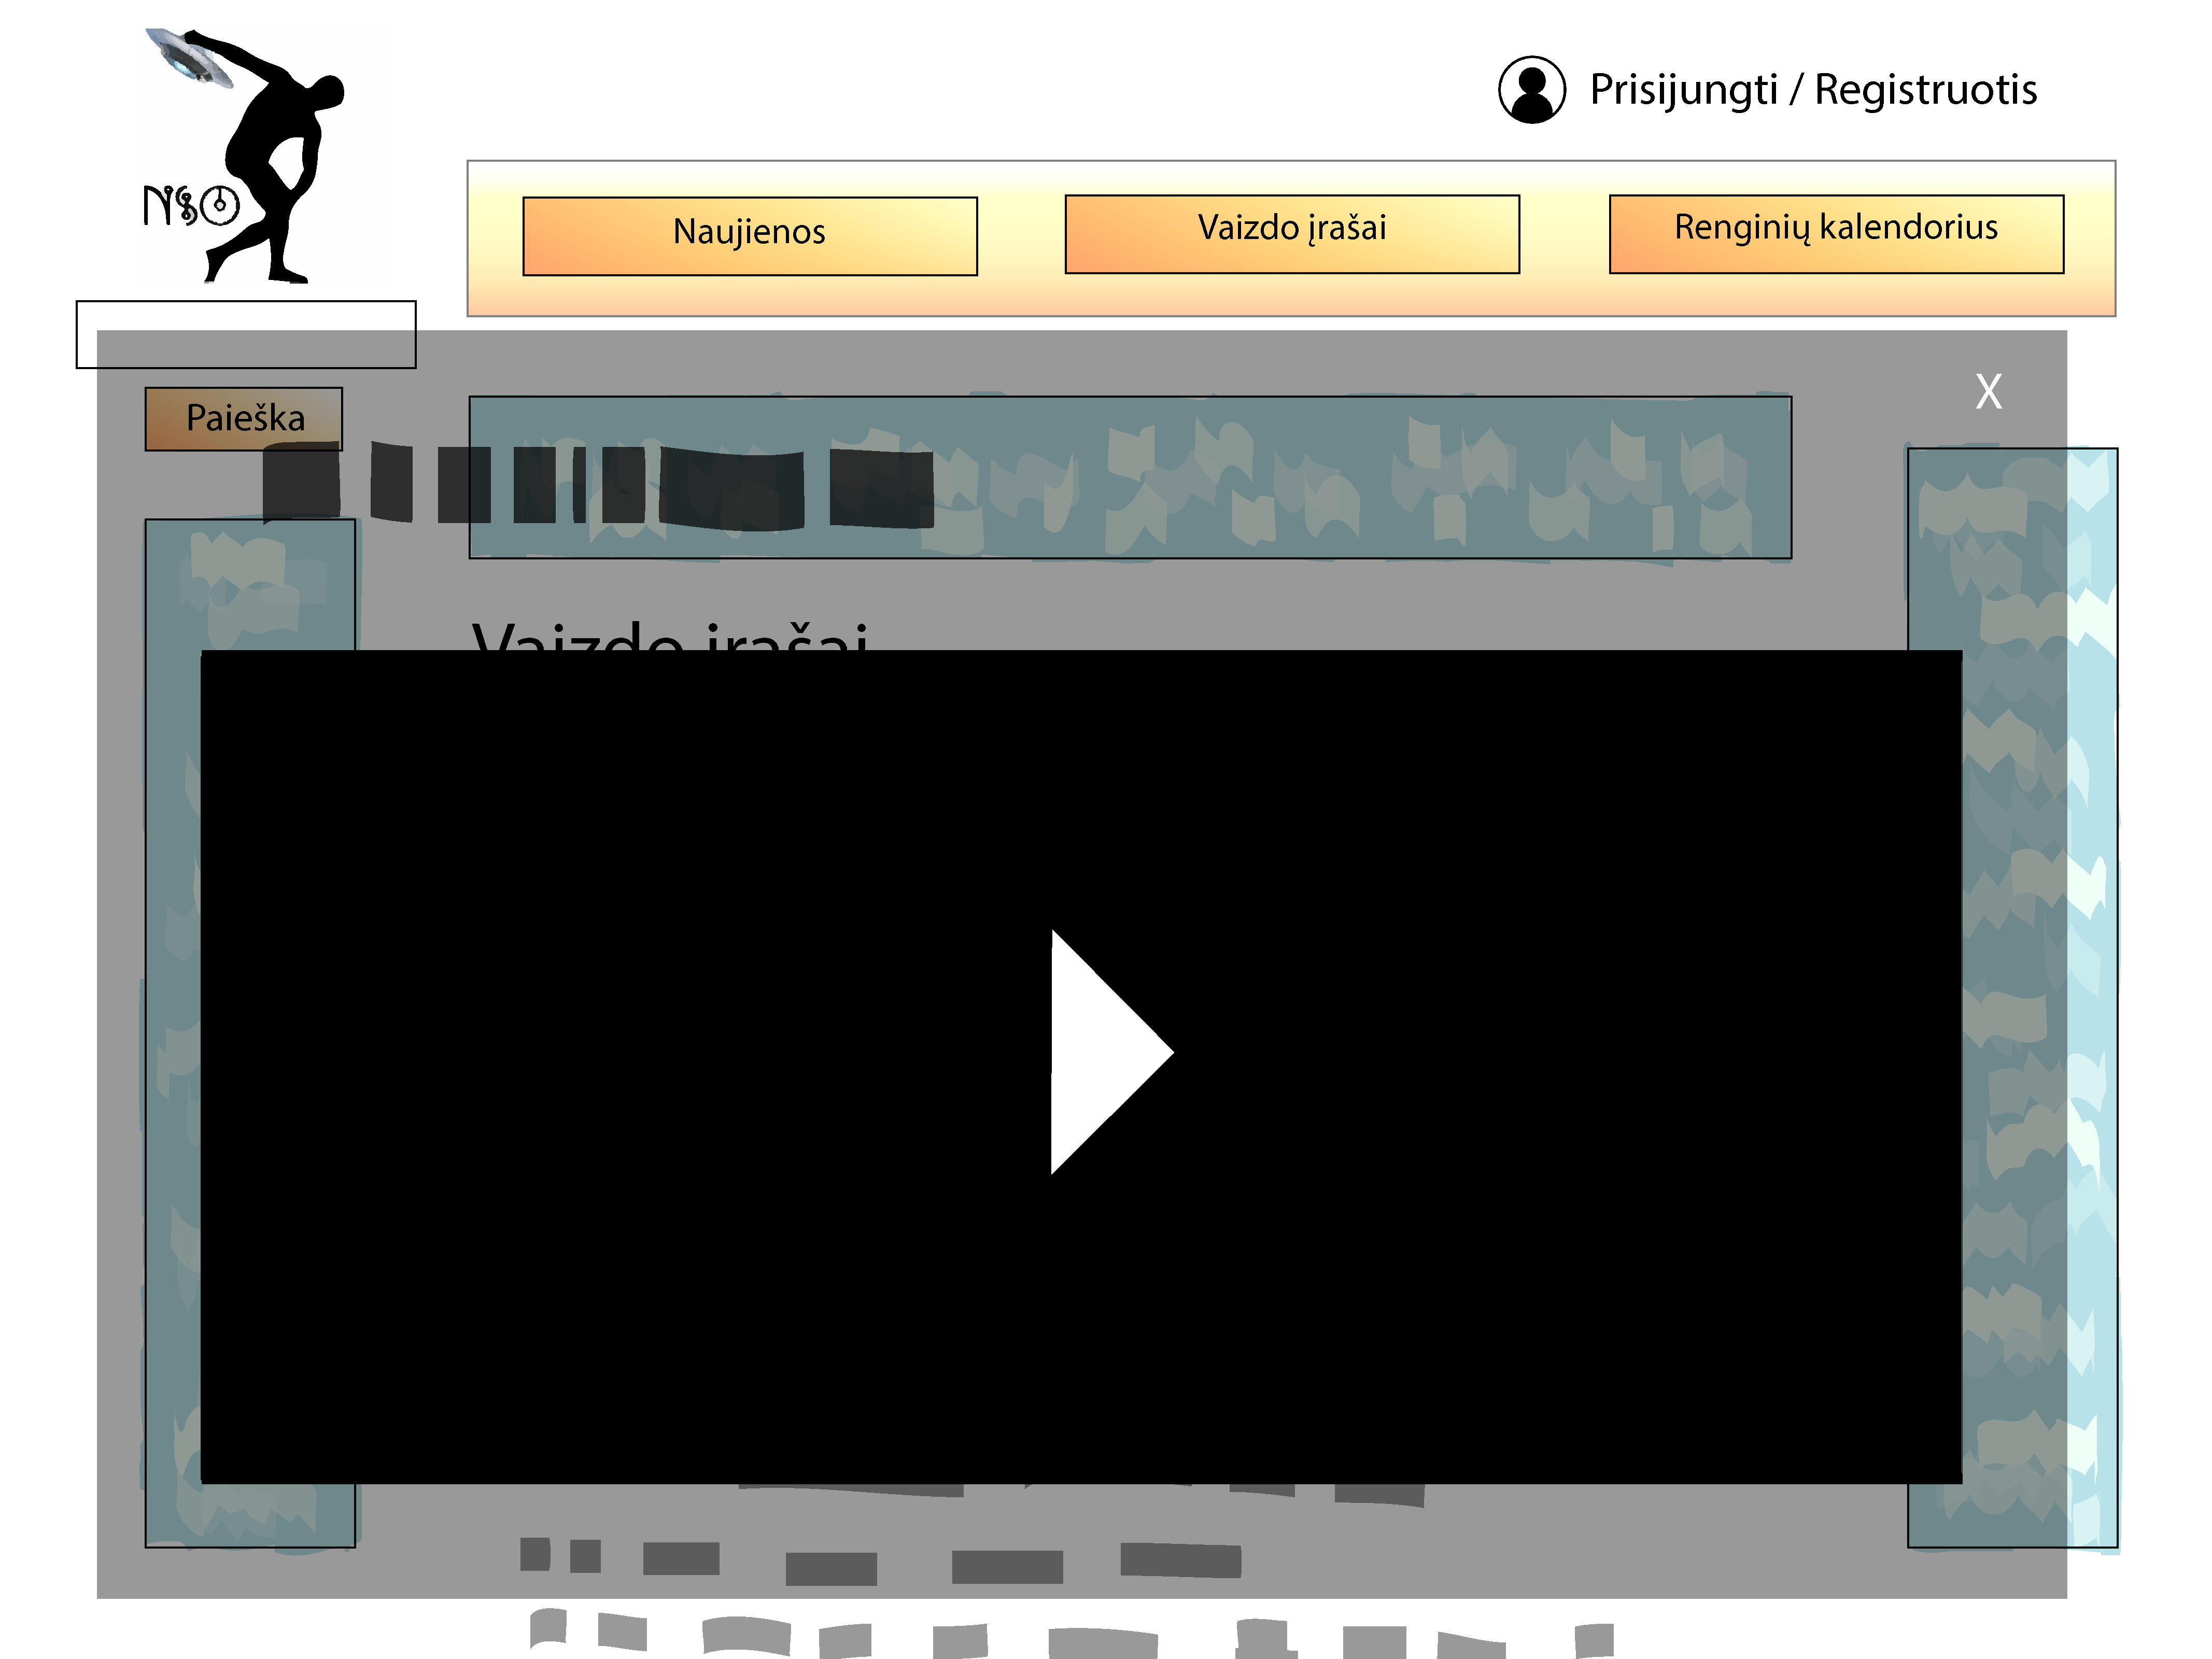
\includegraphics[width=\textwidth, height=8.5cm, keepaspectratio]{img/PSI4/Vaizdoirasai-01.jpg}
					\caption{Vaizdo įrašas}
					\label{fig:uzd_paleistas_vaizdoIrasas}
				\end{figure}
				
			\item \textbf{Pateikti renginio pasiūlymą} \\
					Prisijungęs vartotojas paspaudžia ant mygtuko ,,Pateikti pasiūlymą'', kuris yra navigacijos meniu. Tada vartotojas yra nukeliamas į puslapį su forma, kurioje yra teksto laukas skirtas užpildyti savo pasiūlymo įdėja. Užpildęs įdėjos lauką, vartotojas paspaudžia mygtuką ,,Siųsti'', sistema nusiunčia pranešimą apie įdėją el. paštų administratoriui.
							
					\underline{Alternatyvūs scenarijai:}
					\begin{itemize}
						\item Jei vartotojas nėra prisijungęs, jis privalo užpildyti elektroninio pašto lauką, nes kitaip negalima paspausti mygtuko ,,Siųsti''.
						\item Jei vartotojas įveda netinkamo formato e-paštą ir spaudžia ,,Siųsti'', parodomas pranešimas, kad įvestas netinkamo formato e-paštas.
						\item Jei vartotojas palieką tuščia pasiūlymo lauką ir spaudžia ,,Siųsti'', parodomas pranešimas, kad privaloma įvesti pasiūlymą.
					\end{itemize}
				
			\item \textbf{Registracija} \\
					Vartotojas, norėdamas užsiregistruoti į tinklalapį, spaudžia mygtuką ,,Užsiregistruoti''. Tada vartotojas yra nukeliamas į kitą puslapį, kuriame suveda privaloma informaciją - vartotojo vardą ir slaptažodį. Tuomet, vartotojas spaudžia ,,Baigti'', sistema patikrina ar neegzistuoja vartotojas tokiu vardu, sukuria vartotoją ir peradresuoja naudotoją atgal į pagrindinį puslapį - ,,Renginių kalendorius''.
							
					\underline{Alternatyvūs scenarijai:}
					\begin{itemize}
						\item Vartotojas spaudžia ant užrašo ,,Daugiau informacijos'' ir tada atsiranda papildoma forma su papildomos informacijos laukais (vardas, pavardė, gimimo data, telefono numeris, gyvenamoji vieta). Juos užpildžius spaudžia mygtuką ,,Baigti''. Vartotojas nukeliamas į pagrindinį puslapį.
						\item Vartotojui nepateikus būtinos informacijos arba užpildžius privalomus laukus nekorektiškai, prie atitinkamų laukelių parodoma klaida ir neleidžiama paspausti mygtuką ,,Baigti''.
						\item Jei vartotojas su tokiu vardu jau egzistuoja, parodomas atitinkamas pranešimas.
					\end{itemize}

				\begin{figure}[H]
					\centering
					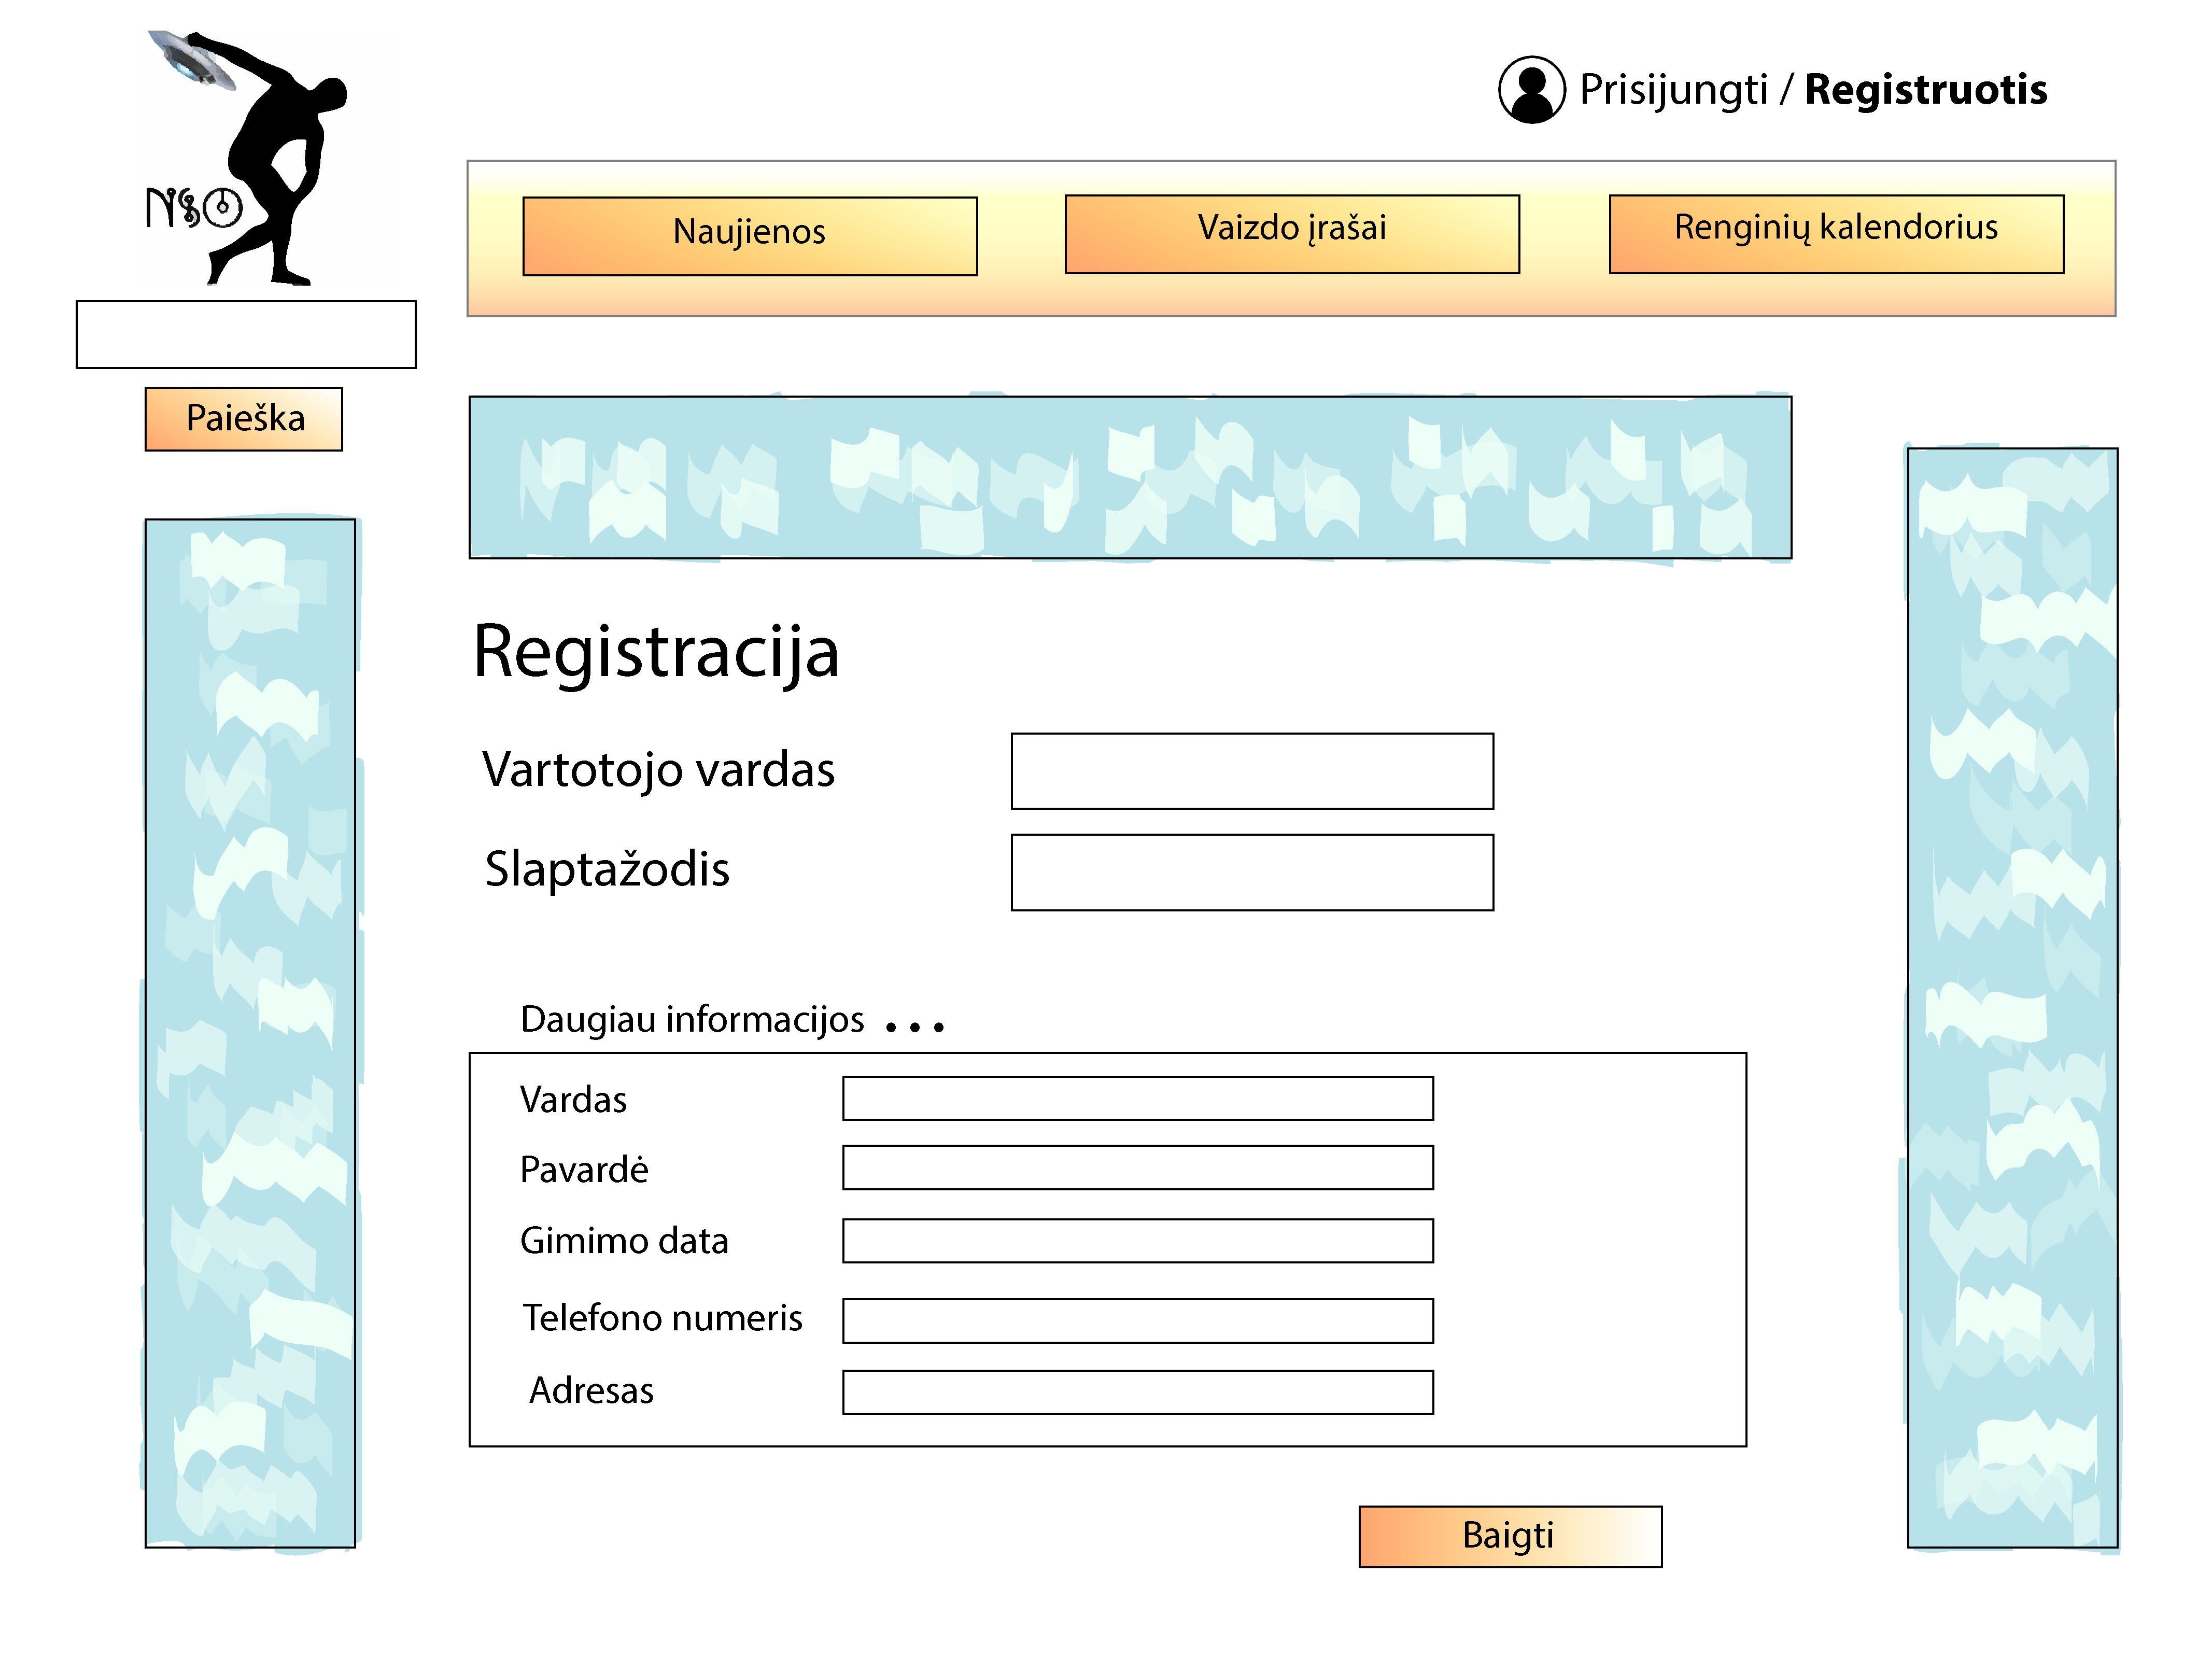
\includegraphics[width=\textwidth]{img/PSI4/registracija-01.jpg}
					\caption{Registracijos langas}
					\label{fig:uzd_registruotis}
				\end{figure}

			\item \textbf{Prisijungti} \\
					Vartotojas spaudžia mygtuką „Prisijungti''. Vartotojas įveda vartotojo vardą ir slaptažodį bei paspaudžia mygtuką ,,Baigti''. Sistema patikrina, ar įvesti duomenys yra teisingi. Sistema vartotojui atidaro prisijungusio vartotojo grafinę sąsają, kurioje vartotojas mato ir gali naudoti prisijungusio vartotojo funkcijas. 
					
				\underline{Alternatyvūs scenarijai:}
				\begin{itemize}
						\item Vartotojui įvedus neteisingą prisijungimo informaciją ar neužpildžius, kurio nors prisijungimo laukelio, sistema paprašo dar kartą įvesti duomenis.
						\item Vartotojui per dažnai bantant įvesti duomenis (10 neteisingų bandymų), ip adresas blokuojamas ir vartojui neleidžiama bandytis jungtis 5min. 
				\end{itemize}

				\begin{figure}[H]
					\centering
					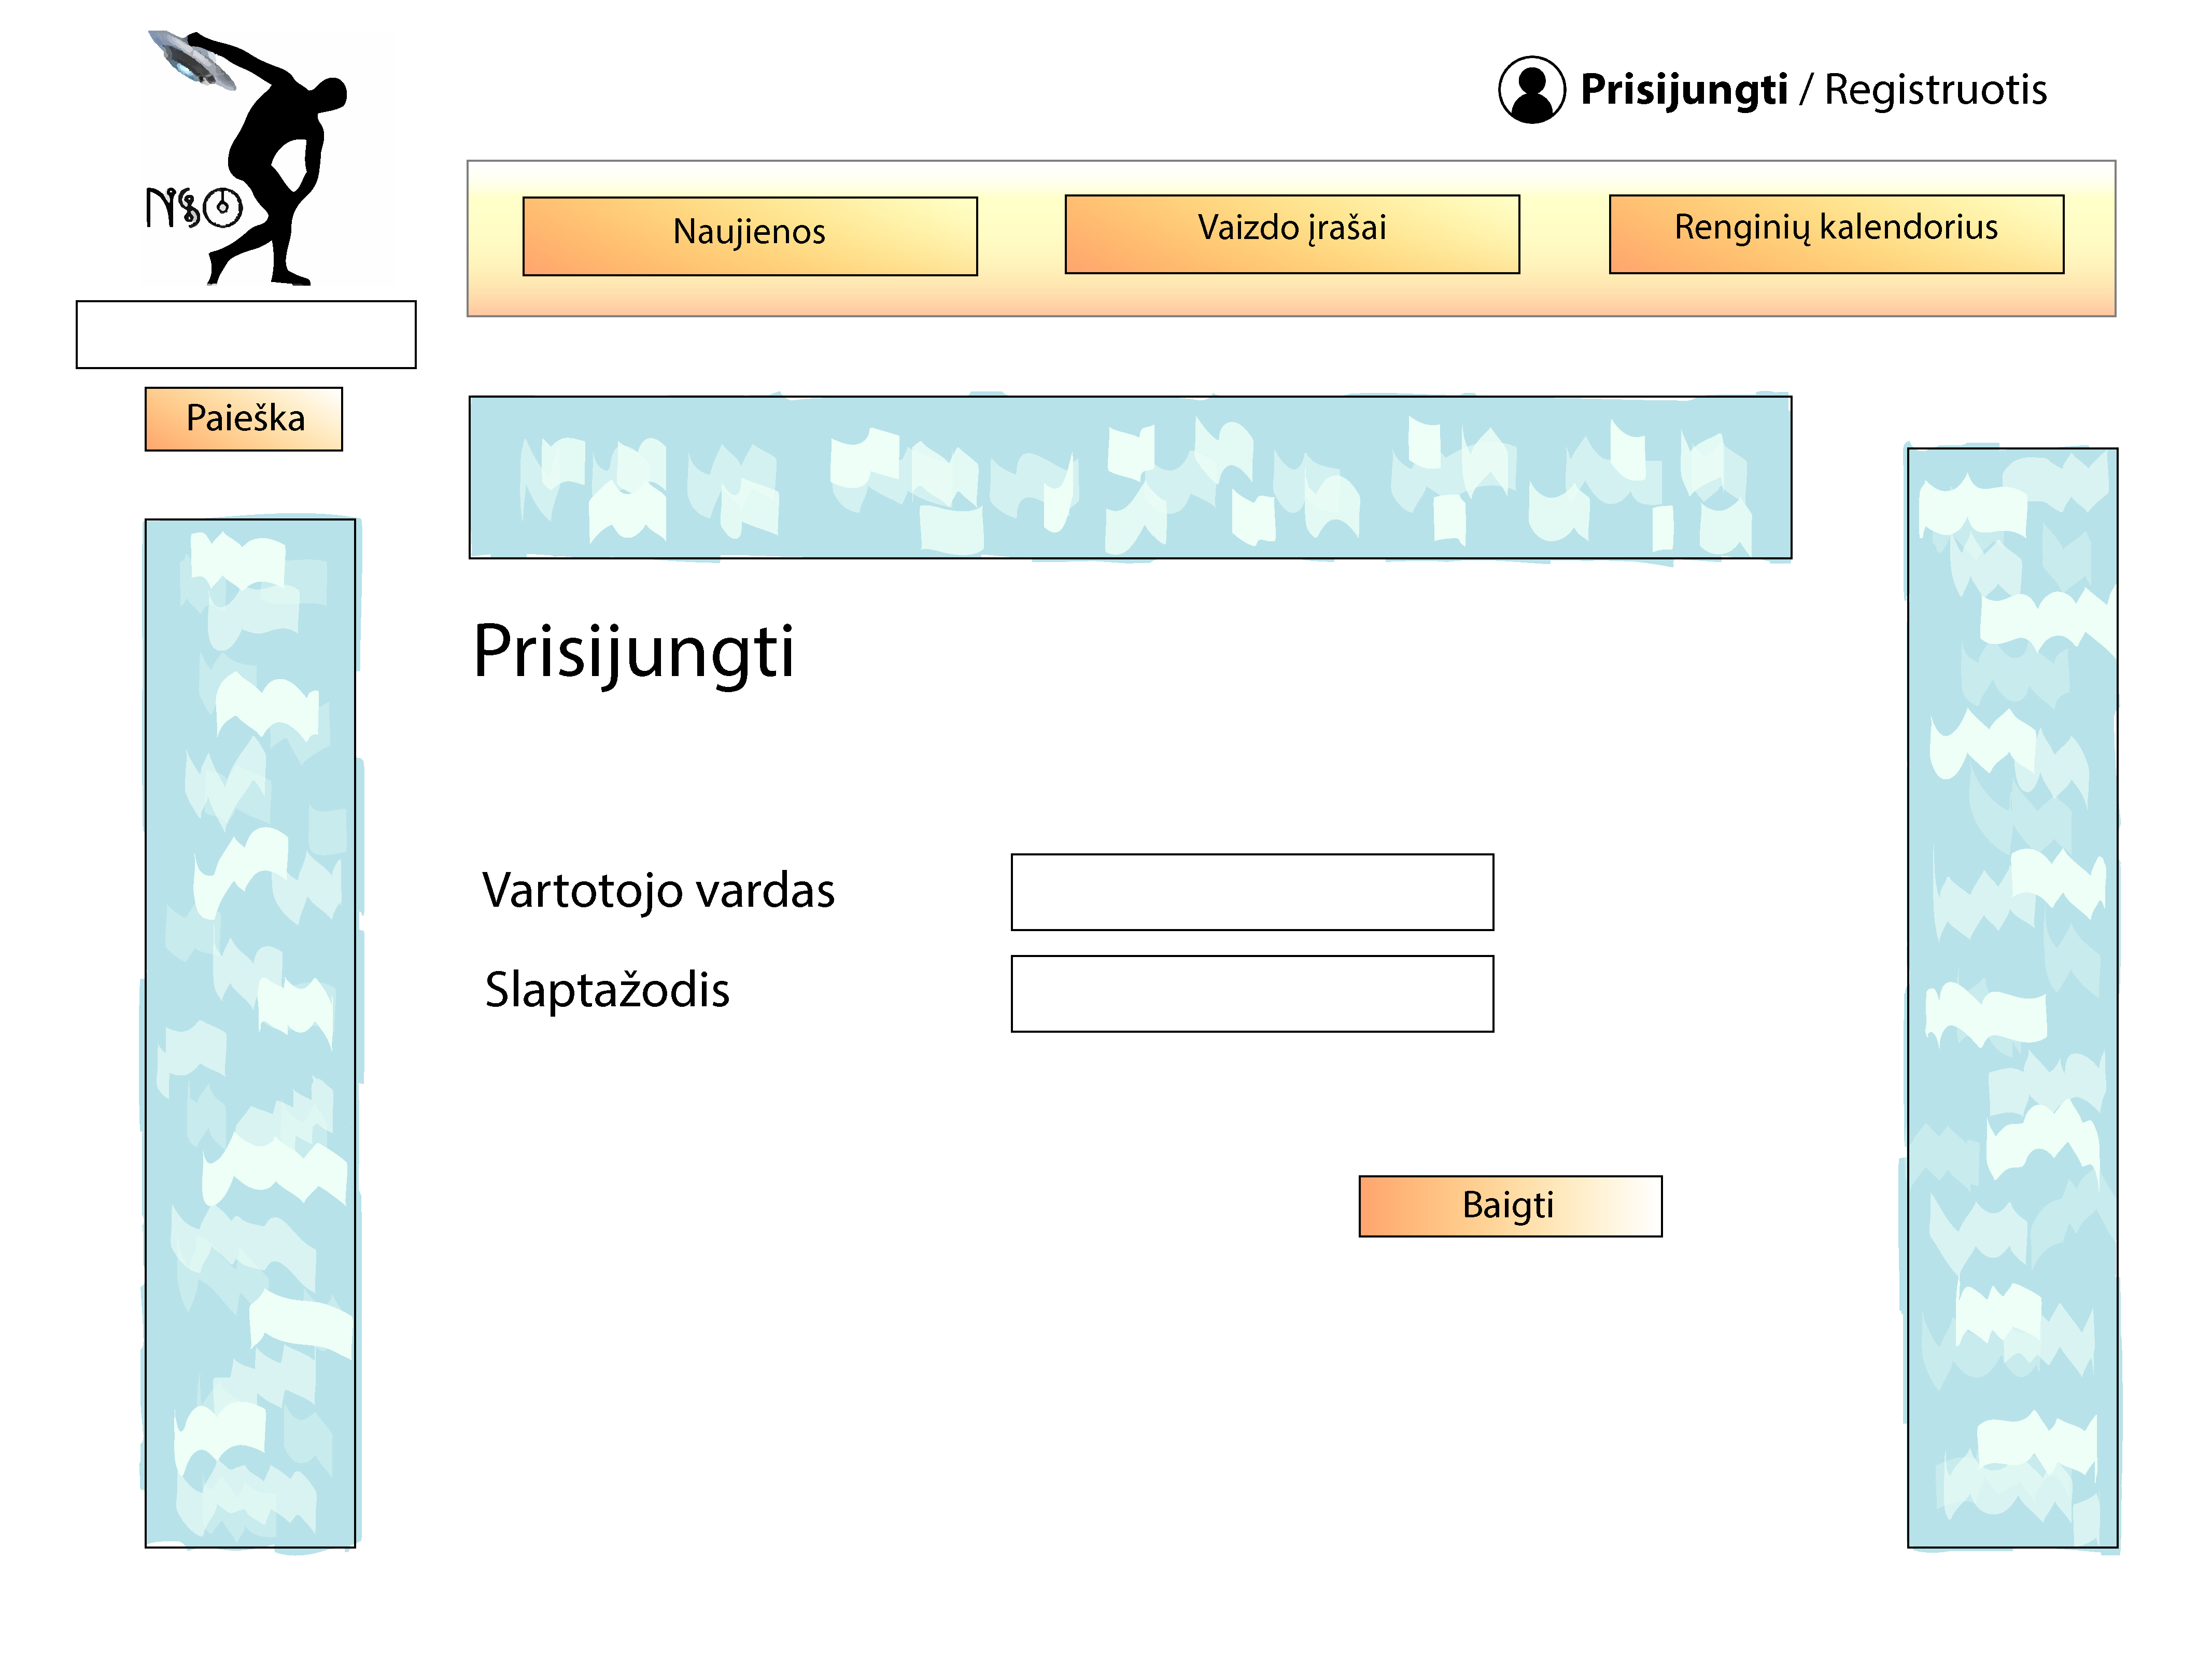
\includegraphics[width=\textwidth]{img/PSI4/Prisijungimas-01.jpg}
					\caption{Prisijungimo langas}
					\label{fig:uzd_prisijungti}
				\end{figure}
			
			\item \textbf{Pirkti bilietus} \\
				Vartotojas, norintis pirkti bilietą į renginį, nueina į norimo renginio puslapį. Paspaudžia mygtuką ,,Pirkti bilietus'' ir tada yra nukreipimas į bilietų pardavimo punktą.
				
				\underline{Alternatyvūs scenarijai:}
				\begin{itemize}
				\item Jei įrenginį bilietai nepardavinėjami, mygtukas ,,Pirkti bilietus'' nerodomas.
				\item Bilietų nebėra į norimą renginį. Mygtukas ,,Pirkti bilietus'' tampa neaktyvus, ant jo užvedus pelyte rodomas pranešimas, kad bilietai išparduoti.
				\end{itemize}
				
			\item \textbf{Registracija į renginį} \\
					Prisijungęs vartotojas spaudžia mygtuką ,,Registruotis''. Vartotojas yra įtraukiamas į renginio dalyvių sąrašą, jam parodomas patvirtinimas apie sėkmingą registraciją.
					
				\underline{Alternatyvūs scenarijai:}
				\begin{itemize}
						\item Registracijos į renginį mygtukas yra neaktyvus, jei renginys jau įvyko.
						\item Registracijos į renginį mygtukas yra neaktyvus, jei užsiregistravo didžiausias galimas dalyvių skaičius.
						\item Registracijos į renginį mygtukas yra nerodomas, jei vartotojas yra jau užsiregistravęs į renginį.
				\end{itemize}
				
			\item \textbf{Kurti komandą} \\
				Prisijungęs vartotojas spaudžia mygtuką ,,Kurti komandą''. Vartotojas įveda komandos pavadinimą ir kviečiamų registruotų vartotojų vardus. Komanda yra sukuriama ir vartotojas gauna pranešimą apie sėkmingai sukurtą komandą.
			
				\underline{Alternatyvūs scenarijai:}
				\begin{itemize}
					\item Metama klaida, jei vartotojas įveda komandos pavadinimą, kuris jau egzistuoja.
					\item Metama klaida, jei vartotojas, kuriantis komandą, į kviečiamų vartotujų sąrašą įtraukia neegzistuojantį vardą.
					\item Mygtukas ,,Kurti komandą'' yra neaktyvus, jei, neįvestas komandos pavadinimas.
					\item Mygtukas ,,Kurti komandą'' yra neaktyvus, jei, nenurodytas nė vienas kviečiamas registruotas vartotojas.
				\end{itemize}

				\begin{figure}[H]
					\centering
					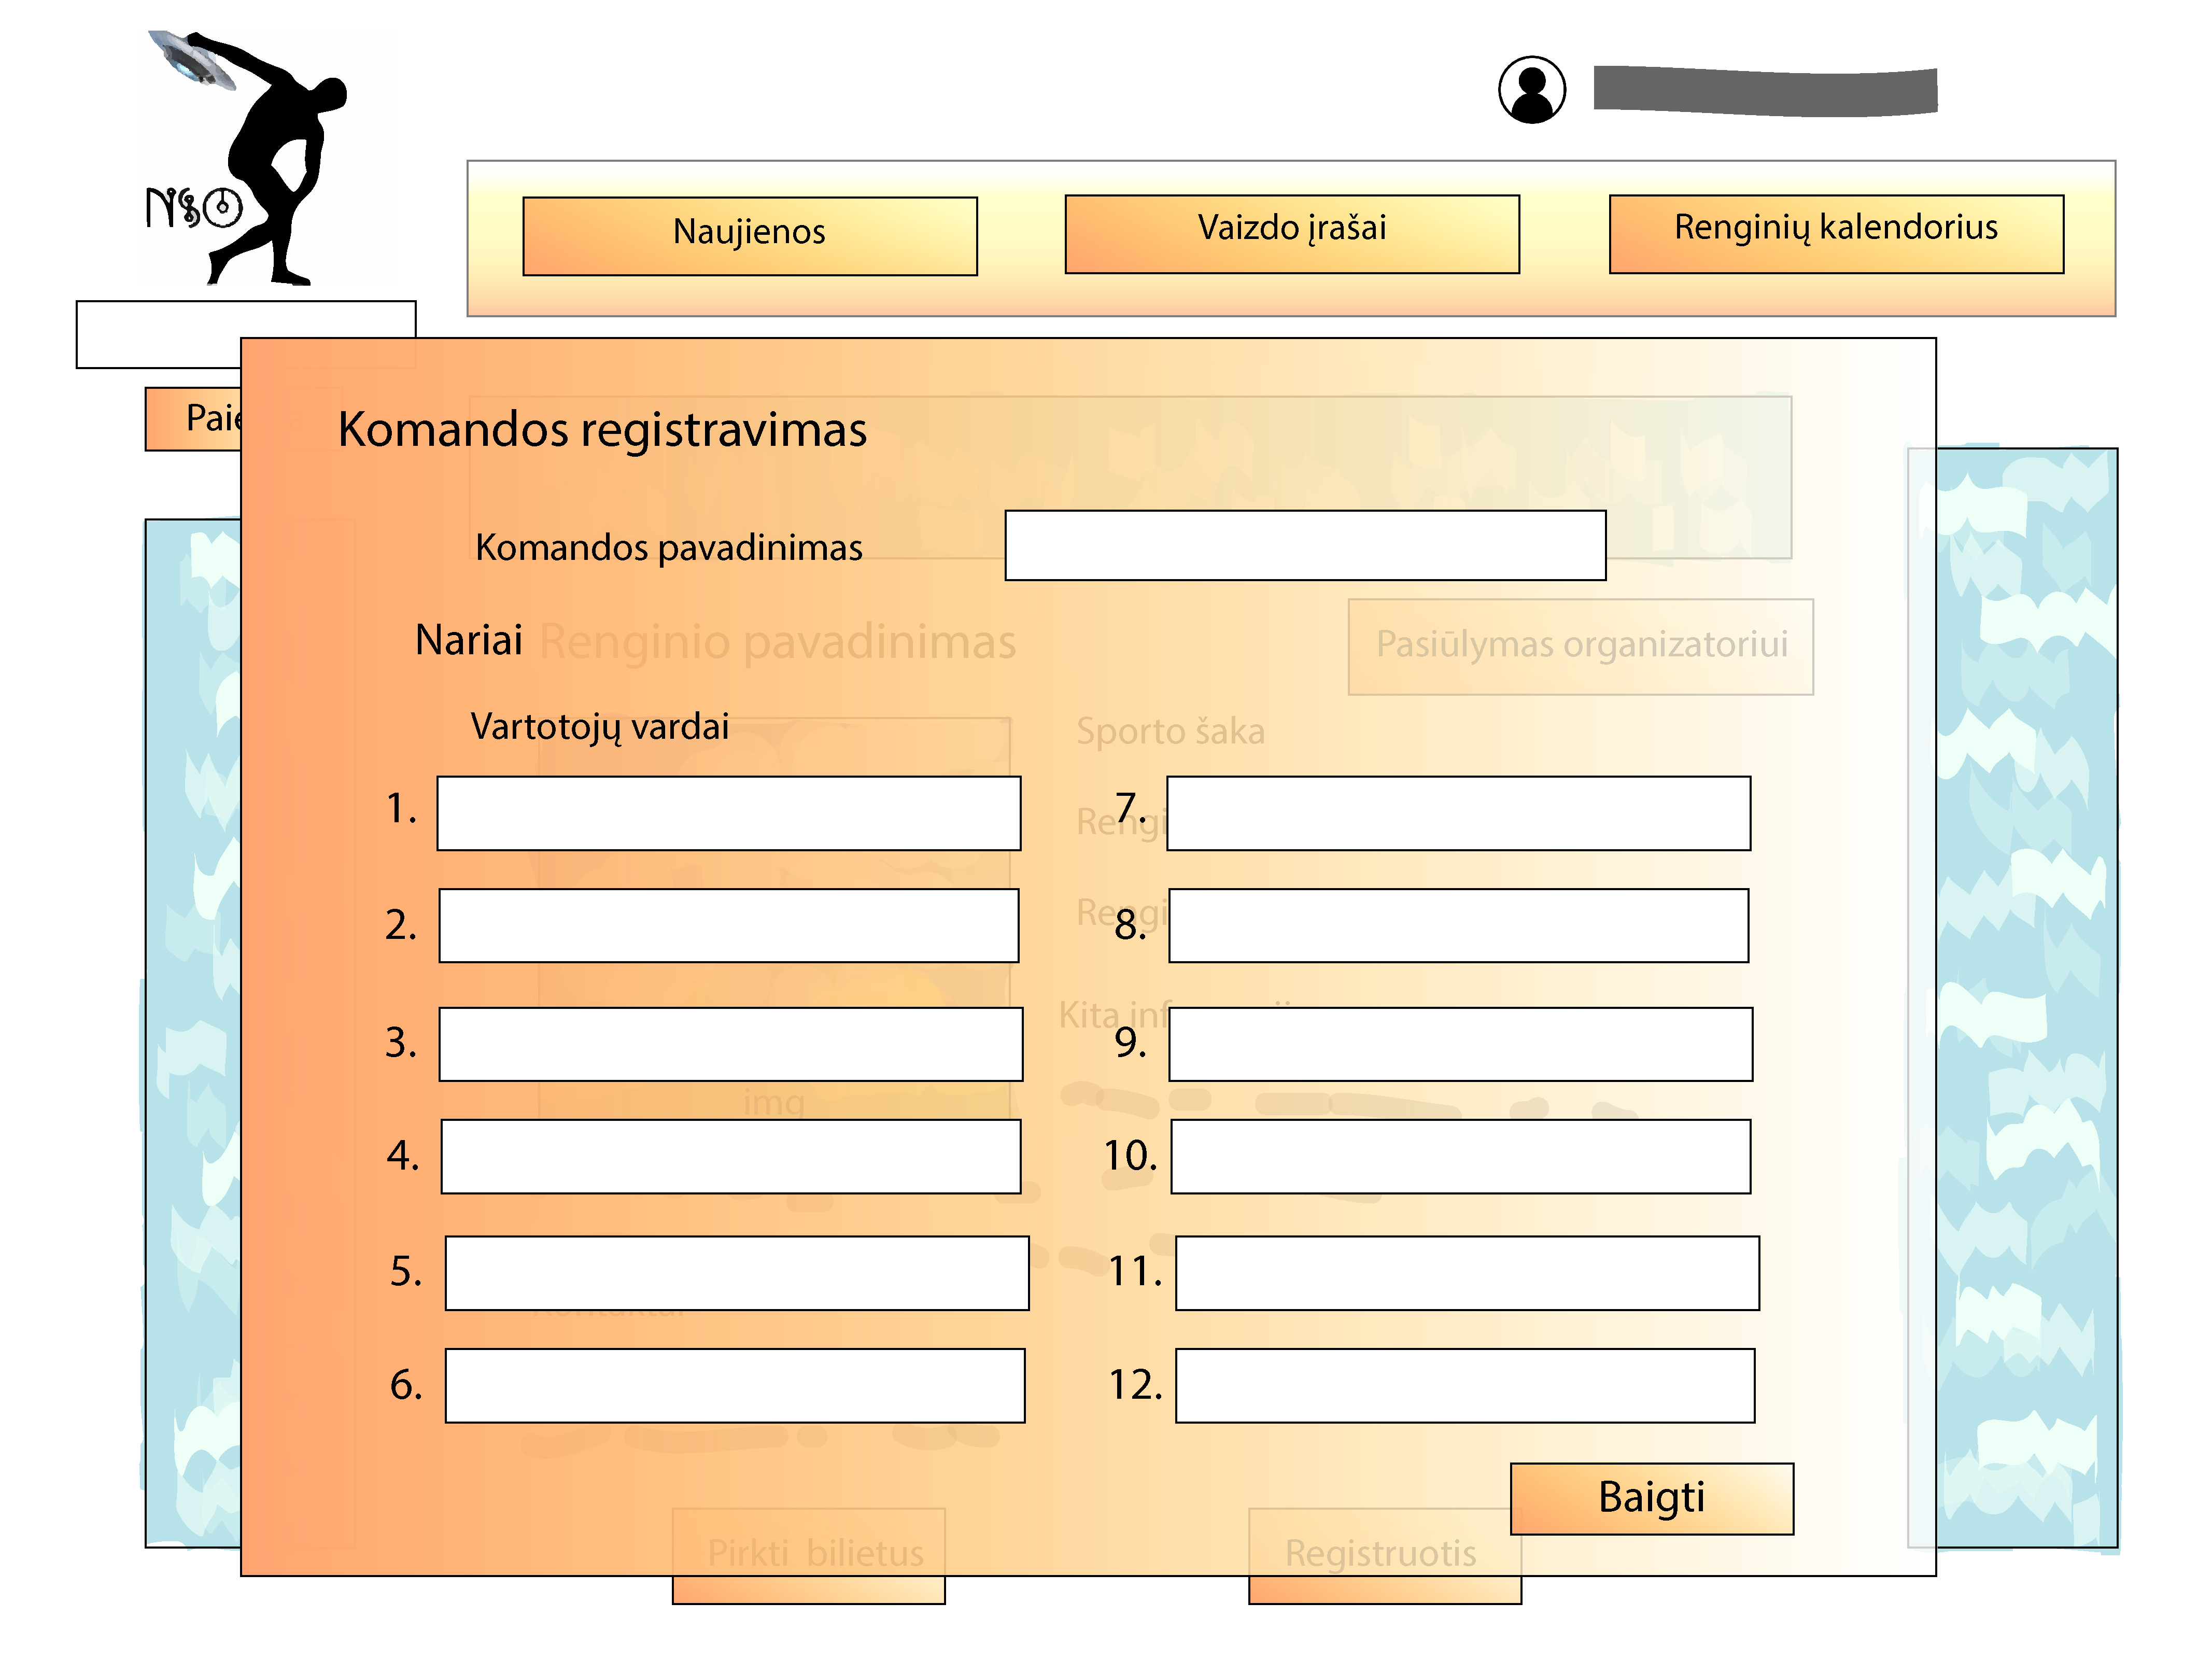
\includegraphics[width=\textwidth]{img/PSI4/renginioPuslapisRegistruotiKomanda-01.jpg}
					\caption{Komandos registracija}
					\label{fig:uzd_registruotiKomanda}
				\end{figure}

			\item \textbf{Priimti kvietimą į komandą} \\
					Vartotojas gavęs pakvietimą į komandą el paštu, paspaudžia nuorodą, kuri nukelia jį į komandos sandaros puslapį, tada ji peržiūri pakvietimą ir nusprendęs kad nori prisijungti prie komandos spaudžia mygtuką ,,Priimti kvietimą''. Sistema prideda vartotoją į komandą ir ištrina pakvietimą.

				\underline{Alternatyvūs scenarijai:}
				\begin{itemize}
					\item Vartotojas paspaudžia mygtuką ištrinti pakvietimą. Sistemą pakvietimą atmeta ir ištrina.
					\item Vartotojas nori sužinoti daugiau informacijos. Tada paspaudęs ant renginio pavadinimo yra nukeliamas į renginio puslapį, kur gali susirinkti daugiau informacijos.
					\item Jeigu komandos vadovas atšaukia kvietima, paspaudus nuorodą, atsirado puslapis su pranešimu, kad kvietimas nebegalioja.
					\item Jei komanda yra ištrinta, paspaudus nuorodą, atsidaro puslapis su pranešimu, kad komanda nebeegzistuoja.
				\end{itemize}

			\item \textbf{Atmesti kvietimą į komandą} \\
				Vartotojas gavęs pakvietimą į komandą el paštu, paspaudžia nuorodą, kuri nukelia jį į komandos sandaros puslapį, peržiūri pakvietimą, nusprendžia kad nenori prisijungti prie komandos, spaudžia mygtuką ,,Atmesti kvietimą''. Sistema ištrina pakvietimą.


				\underline{Alternatyvūs scenarijai:}
				\begin{itemize}
					\item Vartotojas paspaudžia mygtuką ištrinti pakvietimą. Sistemą pakvietimą atmeta ir ištrina.
					\item Jeigu komandos vadovas atšaukia kvietima, paspaudus nuorodą, atsirado puslapis su pranešimu, kad kvietimas nebegalioja.
					\item Jei komanda yra ištrinta, paspaudus nuorodą, atsidaro puslapis su pranešimu, kad komanda nebeegzistuoja.
				\end{itemize}
			
			\item \textbf{Išeiti iš komandos} \\
				Vartotojas būdamas komandos puslapyje paspaudžia mygtuką ,,Išeiti iš komandos''. Iššokusiame lange, kur klausia ,,Ar tikrai norite išeiti iš šios komandos'' paspaudžia mygtuką ,,Taip''.
				
				\underline{Alternatyvūs scenarijai:}
				\begin{itemize}
					\item Vartotojas bando išeiti iš komandos, dalyvaujančios tuo metu vykstančiame renginyje. Tokiu atveju mygtukas  ,,Išeiti iš komandos'' yra neaktyvus ir vartotojui yra skaičiuojami visi taškai kaip ir per varžybas.
				\end{itemize}

			\item \textbf{Pateikti prašymą priimti į komandą} \\
				Prisijungęs vartotojas spaudžia mygtuką ,,Pateiktį prašymą priimti į komandą''. Į teksto lauką vartotojas įveda komandos pavadinimą ir spaudžia mygtuką ,,Pateikti''. Vartotojas yra pridedamas į pasirinktos komandos sąrašą, kaip norintis prisijungti.
				
				\underline{Alternatyvūs scenarijai:}
				\begin{itemize}
					\item Mygtukas ,,Pateikti'' yra neaktyvus ir rodomas klaidos pranešimas, jei įvestas komandos pavadinimas neegzistuoja.
					\item Mygtukas ,,Pateikti'' yra neaktyvus ir rodomas klaidos pranešimas, jei vartotojas jau priklauso komandai, kurios pavadinimą įvedė.
					\item Mygtukas ,,Pateikti'' yra neaktyvus ir rodomas klaidos pranešimas, jei vartotojas jau pateikė prašymą priimti į komandą, kurios pavadinimą įvedė.
					\item Metama klaida, jei komanda, kurios pavadinimas įvestas, yra ištrinta.
				\end{itemize}
				
			\item \textbf{Registruoti komandą į renginį} \\
				Vartotojas spaudžia mygtuką ,,Registruoti komandą''. Vartotojui yra parodomas jo sukurtų komandų sąrašas. Vartotojas pasirenka komandą ir spaudžia mygtuką ,,Registruoti''. Komanda yra pridedama į renginio dalyvių sąrašą.
				
				\underline{Alternatyvūs scenarijai:}
				\begin{itemize}
					\item Mygtukas ,,Registruoti komandą'' yra neaktyvus, jei jau yra viršytas maksimalus dalyvių skaičius.
					\item Mygtukas ,,Registruoti'' yra neaktyvus, jei nepasirinkta komanda.
					\item Jei vartotojas neturi komandų, jam pateikiama nuoroda į komandos kūrimo puslapį.
				\end{itemize}
				
			\item \textbf{Aplikuoti į darbo poziciją} \\
				Prisijungęs vartotojas atsidaro darbo pasiūlymų sąrašą. Atidaro dominančios darbo pozicijos aprašymą. Jei nori aplikuoti į darbo pozicija, kurios aprašymą yra atidaręs, spaudžia mygtuką ,,Aplikuoti''. Į teksto lauką įveda savo žinutę ir, paspaudęs mygtuką ,,Pridėti failą'', prisega iki 10-ies, 2 MB arba mažesnių failų. Spaudžia mygtuką ,,Siųsti''. Aplikaciją į darbo poziciją yra siunčiama administratoriui į e-paštą.
				
				\underline{Alternatyvūs scenarijai:}
				\begin{itemize}
					\item Mygtukas ,,Siųsti'' yra neaktyvus, jei vartotojas paliko tuščią teksto lauką.
					\item Išmetamas pranešimas, jei failas, kurį vartotojas norį įkelti, viršija 2 MB.
					\item Mygtukas ,,Pridėti failą'' yra neaktyvus, jei vartotojas jau įkėlė 10 failų.
				\end{itemize}
				
			\item \textbf{Papildyti asmeninę informaciją} \\
				Prisijungęs vartotojas spaudžia mygtuką ,,Keisti asmeninę informaciją''. Atidaroma forma su teksto laukais, turinčiais etiketes ,,Vardas'', ,,Pavardė'', ,,Gimimo data'', ,,Telefono numeris'', ,,Gyvenamoji vieta'', ,,El-pašto adresas''. Teksto laukuose yra informacija, kurią vartotojas pateikė anksčiau. Vartotojas pakeičia norimą informaciją ir spaudžia ,,Saugoti''. Nauja informacija yra išsaugoma.
				
				\underline{Alternatyvūs scenarijai:}
				\begin{itemize}
					\item Mygtukas ,,Saugoti'' yra neaktyvus, jei vartotojas įveda netinkamą informaciją.
				\end{itemize}

			\item \textbf{Keisti komandos sudėtį} \\
				Prisijungęs vartotojas paspaudžia ant komandos, kurios sudėtį nori keisti, pavadinimo. Atidaromas tos komandos narių, pakviestų vartotojų ir vartotojų, kurie nori prisijungti sąrašas. Prie kiekvieno komandos naro vardo yra mygtukai ,,Ištrinti'' ir ,,Skirti vadovu''. Prie kiekvienio pakviesto vartotojo yra mygtukas ,,Atšaukti kvietimą''. Prie kiekvieno vartotojo, kuris nori prisijungti, vardo yra mygtukai ,,Priimti'' ir ,,Atmesti''. 
				\underline{Alternatyvūs scenarijai:}
				\begin{itemize}
					\item Jei vartotojas spaudžia ,,Priimti'', o pasirinktas vartotojas tuo metu atšaukia prašymą priimti į komandą, pasirinktas vartotojas yra pašalinamas iš sąrašo.
				\end{itemize}
				
			\item \textbf{Pakviesti registruotą vartotoją į komandą}   \\
					Prisijungęs vartotojas paspaudžia ant komandos, kurios vadovo pareigas nori perleisti, pavadinimo. Atidaromas tos komandos narių, pakviestų vartotojų ir vartotojų, kurie nori prisijungti sąrašas.  
					Vartotojas spaudžia, po sąrašu esantį, mygtuką ,,Naujas''. Vartotojui parodomas laukas, į kurį vartotojas įveda kviečiamo registruoto vartotojo vardą. Įvedęs vardą, vartotojas spaudžia mygtuką ,,Kviesti'' ir nurodytam vartotojui yra išsiunčiamas kvietimas.
					
					\underline{Alternatyvūs scenarijai:}
					\begin{itemize}
						\item Jei vartotojas palieka teksto lauką tuščią, mygtukas ,,Kviesti'' yra neaktyvus.
						\item Jei įvedamas neegzistuojantis vardas, metama klaida.
					\end{itemize}
				
			\item \textbf{Perleisti komandos vadovo pareigas kitam vartotojui}   \\
					Prisijungęs vartotojas paspaudžia ant komandos, į kurią nori pakviesti naują narį, pavadinimo. Atidaromas tos komandos narių, pakviestų vartotojų ir vartotojų, kurie nori prisijungti sąrašas. Pasirinkęs komandos narį, kuriam nori perleisti vadovo pareigas, spaudžia prie jo vardo esantį mygtuką ,,Skirti vadovu''. Vartotojui parodomas patvirtinimo langas su mygtuku ,,Patvirtinti''. Vartotojas spaudžia mygtuką ,,Patvirtinti'' ir komandos vadovas yra pakeičiamas.
					
					\underline{Alternatyvūs scenarijai:}
					\begin{itemize}
						\item Administratorius spaudžia mygtuką ,,Skirti vadovu'' ir uždaro patvirtinimo langą. Vadovas nėra pakeičiamas.
					\end{itemize}
				
			\item \textbf{Pridėti naujienas}   \\
					Administratorius paspaudžia ant mygtuko ,,Naujienos'', kuris yra navigacijos meniu. Tada atidaromas puslapis ,,Naujienos'', kurio kairėje pusėje yra pasirinkimas ,,Pridėti naujienas''. Paspaudus ant tų žodžių, atidaroma forma, kurioje reikia užpildyti laukus (privalomi - pavadinimas, tekstas) ir paspausti mygtuką ,,Įkelti''.
					
					\underline{Alternatyvūs scenarijai:}
					\begin{itemize}
						\item Administratoriui neužpildžius privalomų laukų negalima paspausti mygtuko ,,Įkelti'' ir prie laukų, kurie nebuvo užpildyti yra parašoma - ,,Būtina užpildyti''.
					\end{itemize}
			
			\item \textbf{Redaguoti naujienas}   \\
					Administratorius paspaudžia  ant mygtuko ,,Naujienos'', kuris yra navigacijos meniu. Tada atidaromas puslapis ,,Naujienos'', kurio kairėje pusėje yra pasirinkimas ,,Redaguoti naujienas''. Paspaudus ant jų administratorius pasirenka naujienas. Tada paspausti ant pasirinktų naujienų pavadinimo ir atsidaro naujas puslapis su redaguojamais laukais. Redagavus norimus laukus galima paspausti ,,Išsaugoti''.
					
					\underline{Alternatyvūs scenarijai:}
					\begin{itemize}
						\item Administratorius paspaudęs ant naujienų pavadinimo nieko neredaguoja ir nori toliau ieškoti norimų naujienų. Tada jis spaudžia mygtuką ,,Išeiti''.
					\end{itemize}	
			
			\item \textbf{Ištrinti naujienas}   \\
					Administratorius paspaudžia ant mygtuko ,,Naujienos'', kuris yra navigacijos meniu. Tada atidaromas puslapis ,,Naujienos'', kurio kairėje pusėje yra pasirinkimas ,,Ištrinti naujienas''. Paspaudus ant jų, po jais iškrenta pasirinkimas - įvesti naujienų pavadinimą arba pasirinkti iš sąrašo. Paspaudus ant įvesti naujienų pavadinimą, atidaromas naujas puslapis su paieškos laukeliu, į kurį įvedus pavadinimą atidaro visas naujienas turinčias tą pavadinimą. Tada administratorius išsirenka, kurias nori ištrinti. Paspaudžia ant jų ir mygtuką ,,Ištrinti''.
					
					\underline{Alternatyvūs scenarijai:}
					\begin{itemize}
						\item Administratoriui pasirinkus opciją pasirinkti iš sąrašo. Prie esančių puslapio ,,Naujienos'' naujienų atsiranda varnelės opcija, pažymėjus varneles kairėje pusėje galima paspausti mygtuką ,,Ištrinti''.
						\item Administratoriui suvedus netinkamą pavadinimą, kai pasirinktas pasirinkimas įvesti naujienų pavadinimą, atsirandą užrašas ,,Tokių naujienų nėra.''
					\end{itemize}
				
				\begin{figure}[H]
					\centering
					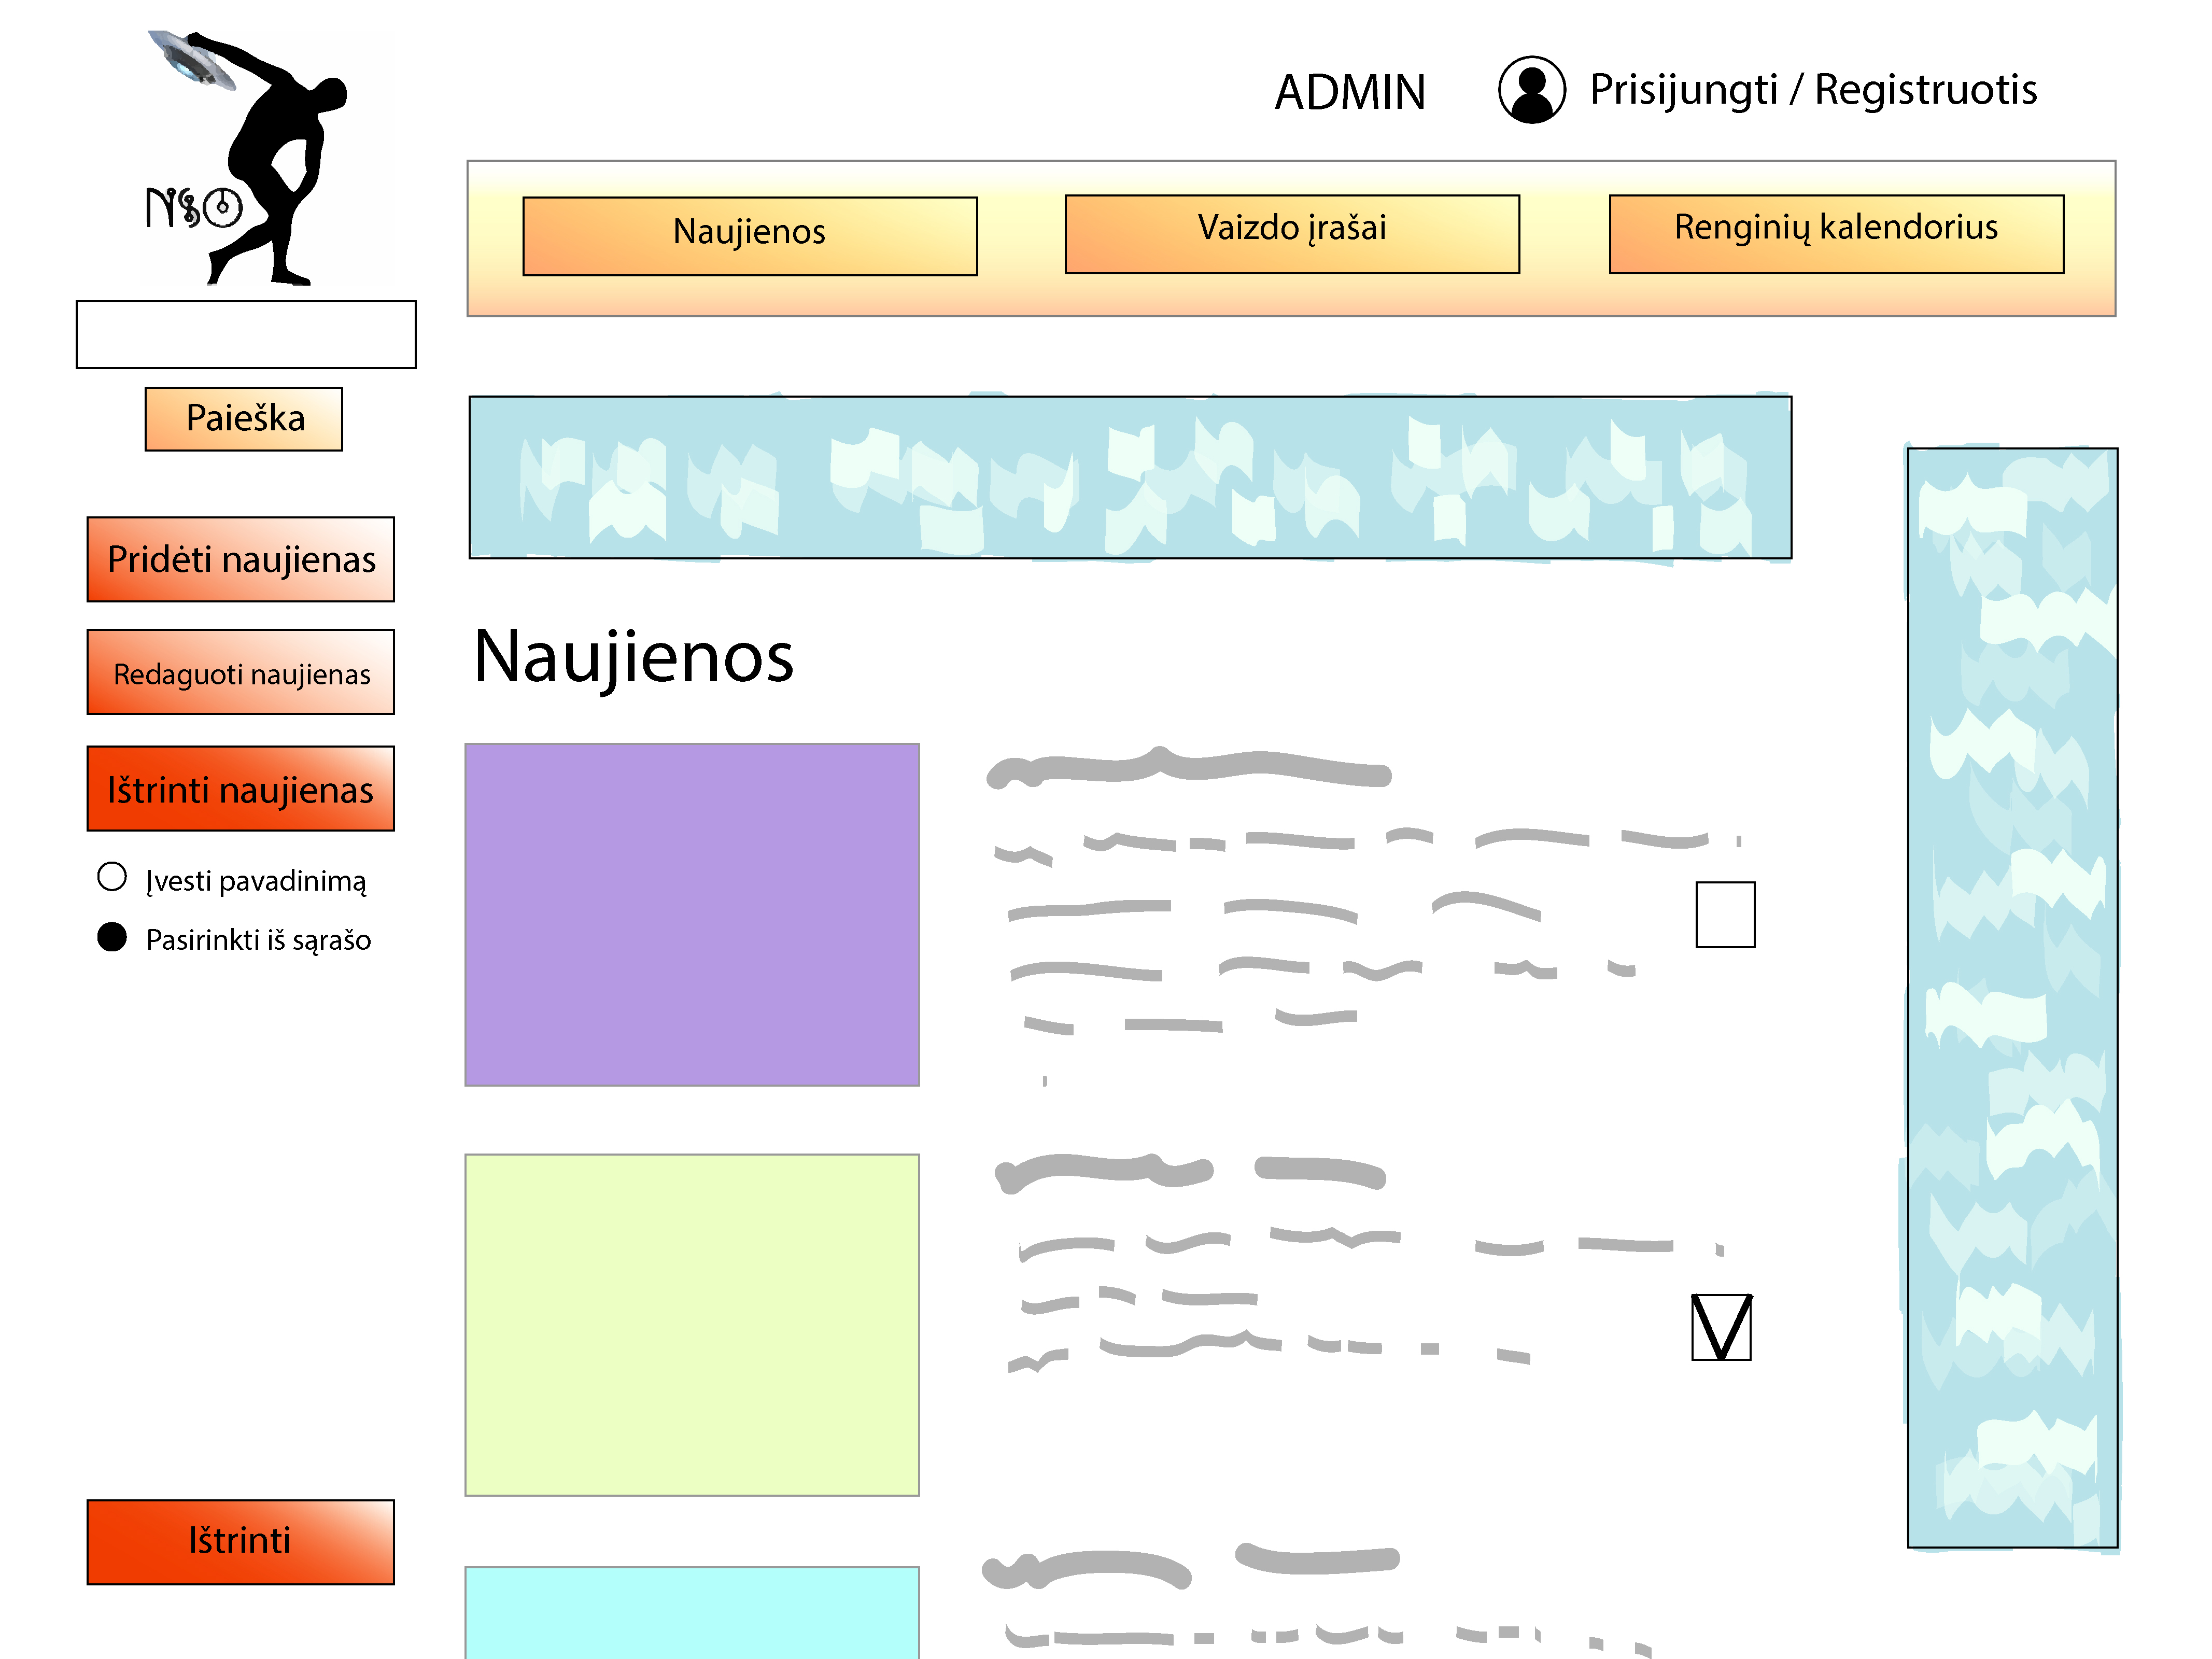
\includegraphics[width=\textwidth, height=8cm, keepaspectratio]{img/PSI4/AdminNaujienos-01.jpg}
					\caption{Administratoriaus prieiga puslapiui ,,Naujienos''}
					\label{fig:uzd_admin_puslapisNaujienos}
				\end{figure}
				
			\item \textbf{Pridėti renginį}   \\
					Administratorius paspaudžia ant mygtuko ,,Renginių kalendorius'', kuris yra navigacijos meniu. Atidaromas puslapis ,,Renginių kalendorius'', kurio kairėje pusėje yra pasirinkimas ,,Pridėti renginį''. Paspaudus ant jo atsidaro naujas puslapis su forma, kurioje yra laukai (renginio pavadinimas, sporto šaka, vienos komandos dydis (intervalas), maksimalus dalyvių skaičius, registravimosi termino data, renginio data, vieta, bilietu pardavimo vieta). Įvedus visus reikalingus laukus, administratorius paspaudžia mygtuką ,,Baigti''.
					
					\underline{Alternatyvūs scenarijai:}
					\begin{itemize}
						\item Administratorius nesuveda visų privalomų laukų. Jam neleidžia paspausti mygtuko ,,Baigti'' ir prie atitinkamų laukų rašoma klaida.
					\end{itemize}
				
			\item \textbf{Redaguoti renginį}   \\
					Administratorius spaudžia ant mygtuko ,,Renginių kalendorius'', kuris yra navigacijos meniu. Tada atidaromas puslapis ,,Renginių kalendorius''. Kalendoriuje administratorius pasirenka renginį, kurį nori redaguoti. Prie renginio spaudžia mygtuką ,,Redaguoti''. Paspaudus ant jo atsidaro naujas puslapis su renginio informacijos redagavimo forma. Laukai yra užpildyti anksčiau įvesta informacija. Pakeitęs norimus laukus, administratorius paspaudžia mygtuką ,,Baigti''.
					
					\underline{Alternatyvūs scenarijai:}
					\begin{itemize}
						\item Administratorius nesuveda visų privalomų laukų. Jam neleidžia paspausti mygtuko ,,Baigti'' ir prie atitinkamų laukų rašoma klaida.
					\end{itemize}
				
				\begin{figure}[H]
					\centering
					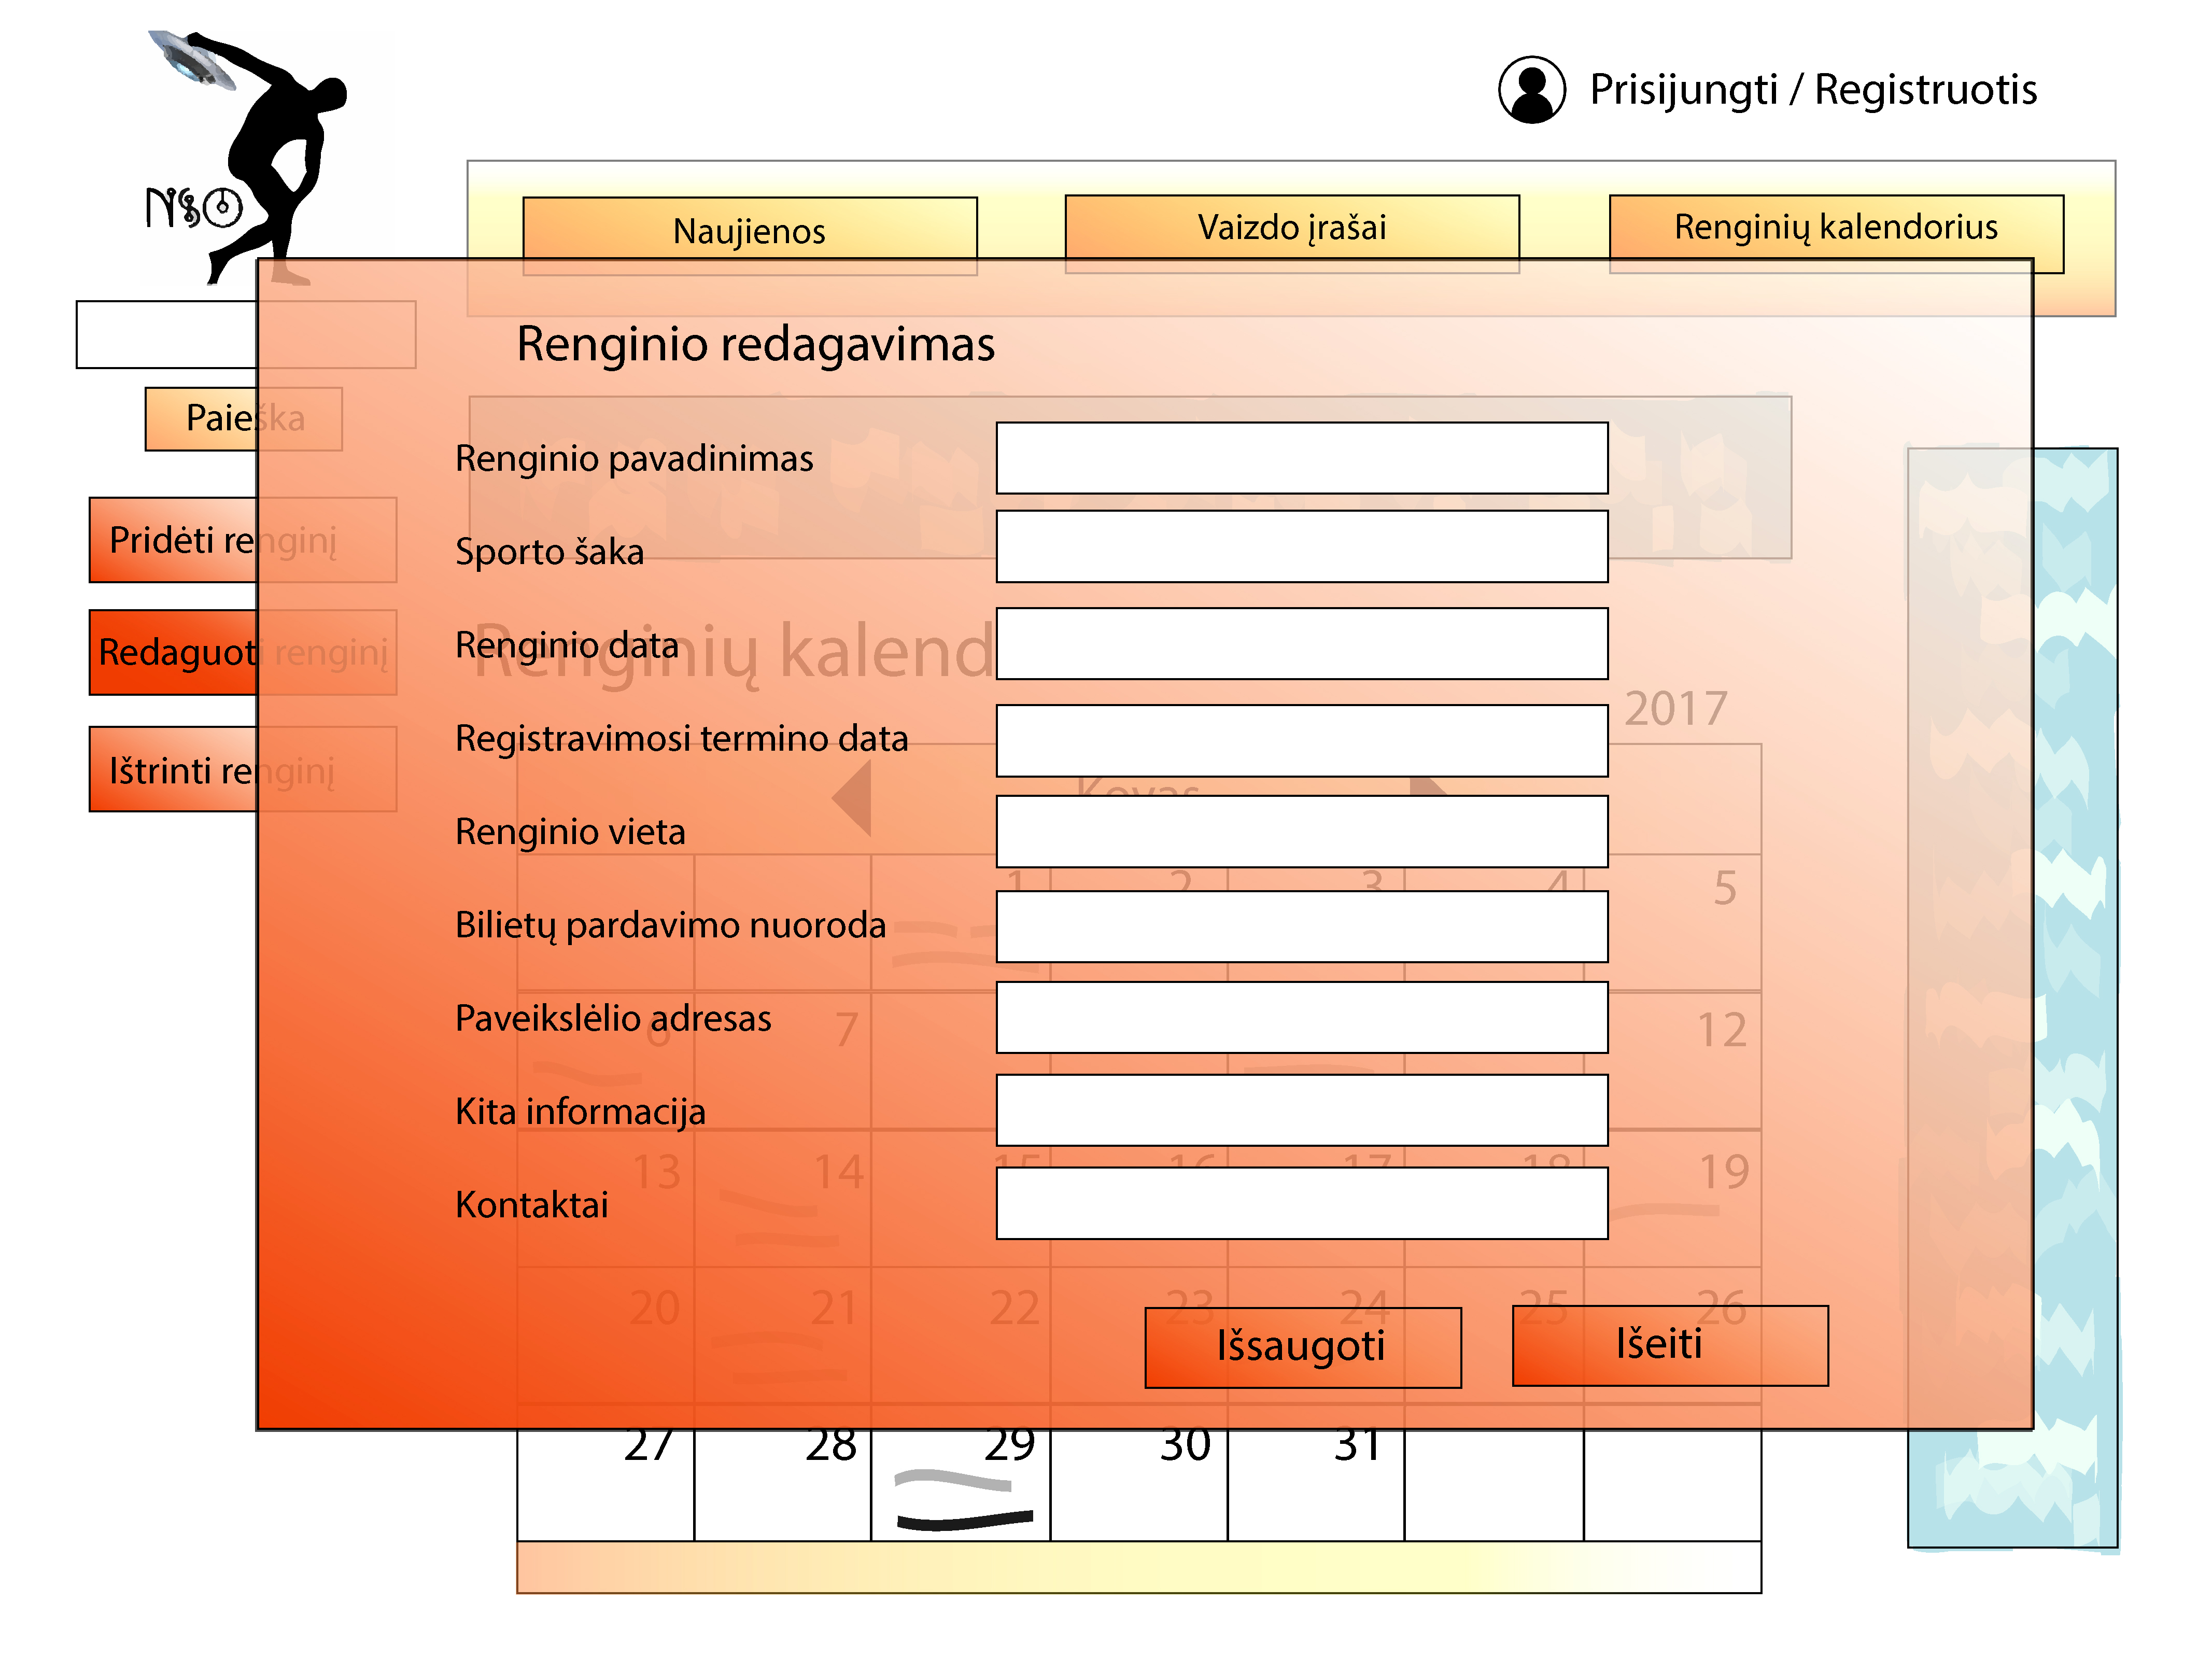
\includegraphics[width=\textwidth, height=8cm, keepaspectratio]{img/PSI4/AdminRenginioKalendorius-01.jpg}
					\caption{Administratoriaus prieiga puslapiui ,,Renginio kalendorius''}
					\label{fig:uzd_admin_renginioKalendorius}
				\end{figure}
				
			\item \textbf{Ištrinti renginį}   \\
					Administratorius spaudžia ant mygtuko ,,Renginių kalendorius'', kuris yra navigacijos meniu. Tada atidaromas puslapis ,,Renginių kalendorius''. Kalendoriuje administratorius pasirenka renginį, kurį nori ištrinti. Prie renginio spaudžia mygtuką ,,Ištrinti''. Sistema parodo patvirtinimo dialogą, administratorius patvirtina ištrinimą, sistema išsiunčia visiems užregistravusiems renginio dalyviams pranešimą kad renginys atšauktas, ir renginys yra ištrinamas.
					
					\underline{Alternatyvūs scenarijai:}
					\begin{itemize}
						\item Jei administratorius atsiradus dialogui atšaukia ištrinimą, dialogas pašalinamas ir parodomas renginio puslapis.
					\end{itemize}
				
			\item \textbf{Pridėti rezultatus}   \\
					Administratorius spaudžia ant mygtuko ,,Renginių kalendorius'', kuris yra navigacijos meniu. Tada atidaromas puslapis ,,Renginių kalendorius''. Kalendoriuje administratorius pasirenka renginį, kurio rezultatus nori pridėti. Prie renginio spaudžia mygtuką ,,Rezultatai''. Paspaudus ant jo parodoma renginio formatą atitinkanti lentelė, kurią galima užpildyti renginio rezultatais. Administratorius suveda renginio rezultatus ir spaudžia mygtuką ,,Patvirtinti''.
					
					\underline{Alternatyvūs scenarijai:}
					\begin{itemize}
						\item Metamos klaidos, jei rezultatai yra vedami neteisingai (pvz.: kai į skaitinius laukus bandomos įvesti raidės).
						\item Mygtukas ,,Rezultatai'' yra neaktyvus, jei renginys dar neprasidėjo.
						\item Mygtukas ,,Patvirtinti'' yra neaktyvus, jei administratorius rezultatų nesuvedė.
					\end{itemize}
					
			\item \textbf{Redaguoti rezultatus}   \\
					Administratorius spaudžia ant mygtuko ,,Renginių kalendorius'', kuris yra navigacijos meniu. Tada atidaromas puslapis ,,Renginių kalendorius''. Kalendoriuje administratorius pasirenka renginį, kurio rezultatus nori pridėti. Prie renginio spaudžia mygtuką ,,Rezultatai''. Paspaudus ant jo parodoma renginio formatą atitinkanti lentelė, kurioje galima matyti ir redaguoti renginio rezultatais. Administratorius pakeičia rezultatus ir spaudžia mygtuką ,,Patvirtinti''.
					
					\underline{Alternatyvūs scenarijai:}
					\begin{itemize}
						\item Metamos klaidos, jei rezultatai yra vedami neteisingai (pvz.: kai į skaitinius laukus bandomos įvesti raidės).
						\item Mygtukas ,,Patvirtinti'' yra neaktyvus, jei administratorius nepadarė pakeitimų.
					\end{itemize}
				
			\item \textbf{Ištrinti rezultatus}   \\
					Administratorius spaudžia ant mygtuko ,,Renginių kalendorius'', kuris yra navigacijos meniu. Tada atidaromas puslapis ,,Renginių kalendorius''. Kalendoriuje administratorius pasirenka renginį, kurio rezultatus nori pridėti. Prie renginio spaudžia mygtuką ,,Rezultatai''. Paspaudus ant jo parodoma renginio formatą atitinkanti lentelė, kurioje galima matyti ir redaguoti renginio rezultatais. Administratorius spaudžia mygtuką ,,Išvalyti'' ir mygtuką ,,Patvirtinti''.
					
					\underline{Alternatyvūs scenarijai:}
					\begin{itemize}
						\item Mygtukas ,,Išvalyti'' yra neaktyvus, jei rezultatų lentelė yra tuščia.
						\item Mygtukas ,,Patvirtinti'' yra neaktyvus, jei administratorius nepadarė pakeitimų.
					\end{itemize}
				
			\item \textbf{Pridėti vaizdo įrašą}   \\
					Administratorius spaudžia ant mygtuko “Vaizdo įrašai”, kuris yra navigacijos meniu. Paspaudus ant jo parodomas renginio vaizdo įrašų sąrašas. Administratorius spaudžia mygtuką “Pridėti”. Atsidaro naujas langas su lauku į kurį galima vaizdo įrašo nuorodą bei mygtuku “Įkelti”, kurį paspaudus leidžiama pasirinkti vaizdo įrašą iš kompiuterio. Administratorius įveda vaizdo įrašo nuorodą arba spaudžia mygtuką “Įkelti” ir pasirenka failą iš kompiuterio. Administratorius spaudžia mygtuką “Išsaugoti”.
					
					\underline{Alternatyvūs scenarijai:}
					\begin{itemize}
						\item Metama klaida, jei bandoma įkelti failą iš kompiuterio ir įvesti nuorodą.
						\item Metama klaida, jei bando talpinti netinkamo formato failą.
					\end{itemize}
				
				\begin{figure}[H]
					\centering
					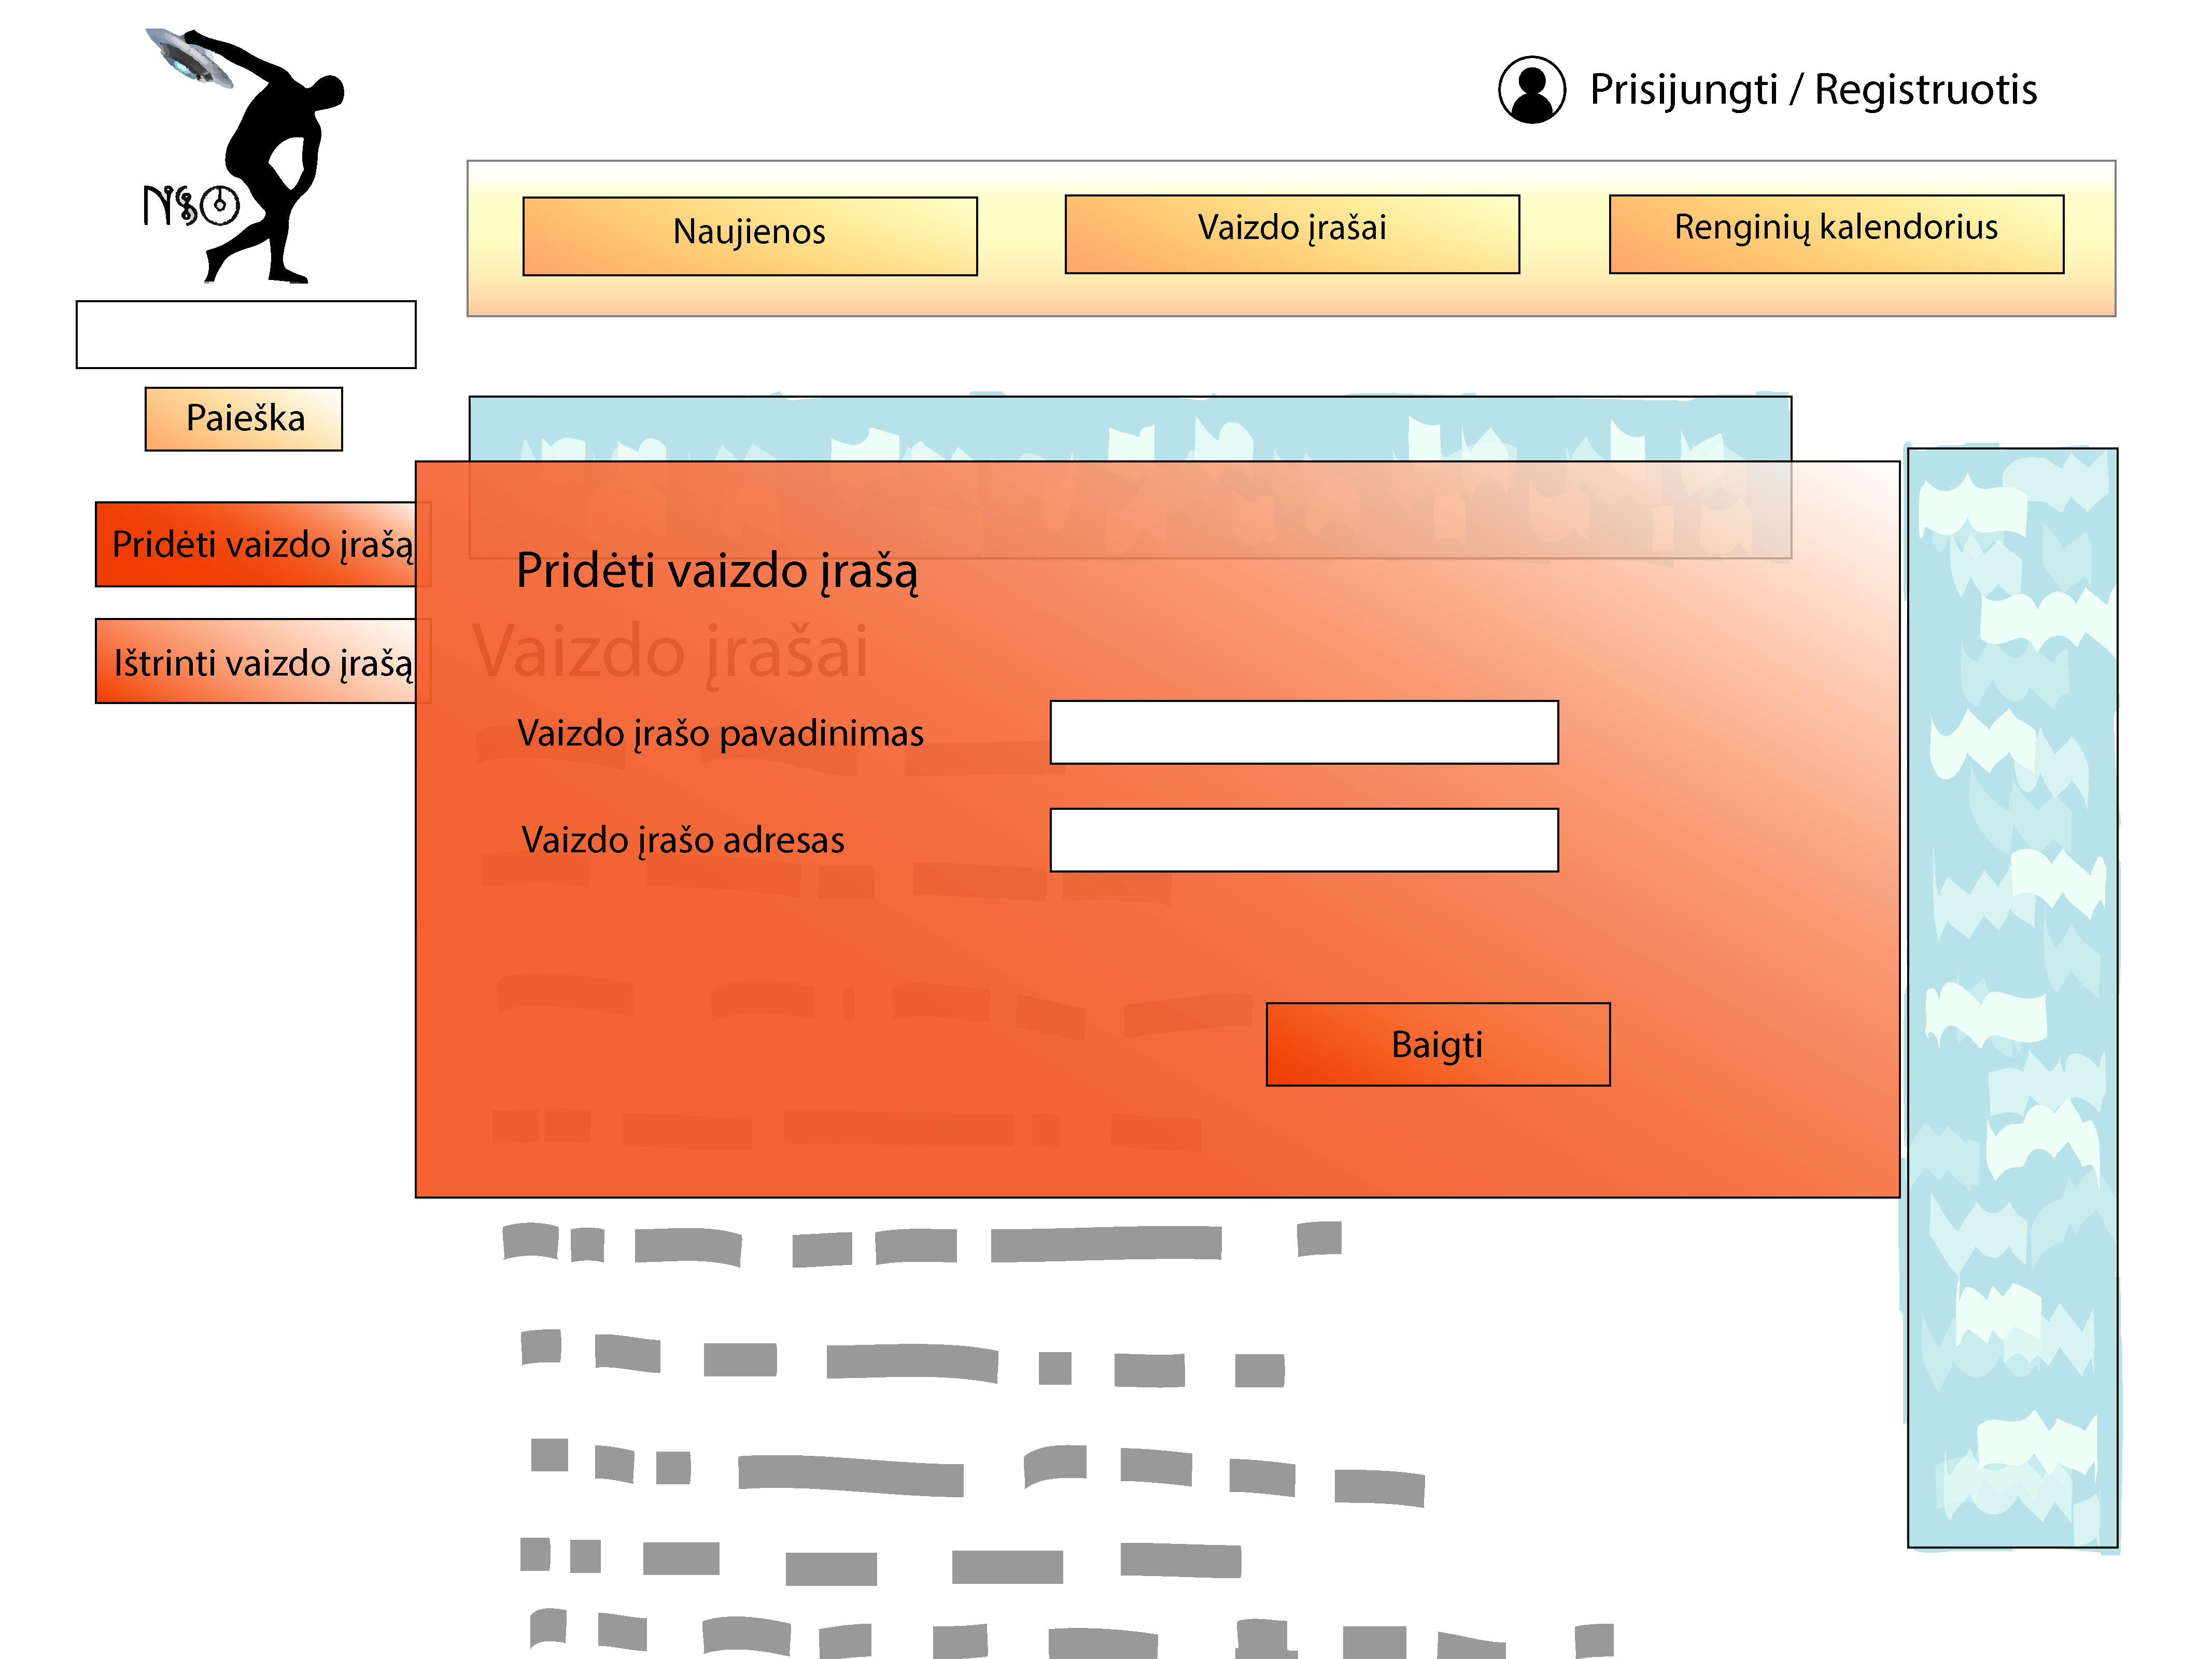
\includegraphics[width=\textwidth, height=8cm, keepaspectratio]{img/PSI4/AdminVaizdoirasai-01.jpg}
					\caption{Administratoriaus prieiga puslapiui ,,Vaizdo įrašai''}
					\label{fig:uzd_admin_vaizdoIrasas}
				\end{figure}
					
			\item \textbf{Ištrinti vaizdo įrašą}   \\
					Administratorius spaudžia ant mygtuko “Vaizdo įrašai”, kuris yra navigacijos meniu. Paspaudus ant jo parodomas renginio vaizdo įrašų sąrašas. Prie kiekvieno vaizdo įrašo yra mygtukas “Ištrinti”. Administratorius spaudžia mygtuką “Ištrinti” prie pasirinkto vaizdo įrašo. Parodomas langas, kuriame prašoma patvirtinti, kad nori ištrinti vaizdo įrašą. Administratorius spaudžia mygtuką “Patvirtinti”. Vaizdo įrašas ištrinamas.
					
					\underline{Alternatyvūs scenarijai:}
					\begin{itemize}
						\item Administratorius spaudžia mygtuką ,,Ištrinti'' ir uždaro patvirtinimo langą. Vaizdo įrašas nėra ištrinamas.
					\end{itemize}
					
			\item \textbf{Apriboti, blokuoti, ištrinti vartotojus}   \\
					Administratorius užeina į atitinkamo vartotojo puslapį pasirenka, ką nori daryti ir paspaudžia mygtukus ,,Apriboti prieiga'', ,,Blokuoti prieigą'', ,,Ištrinti vartotoją''. Pasirinkęs ,,Apriboti prieiga'' arba ,,Blokuoti prieigą'' administratorius iššokusiame lange pasirenka iki kada jis nori, kad tai galiotų ir spaudžia ,,Patvirtinti''. Jei administratorius paspaudžia ,,Ištrinti vartotoją'', jis turi papildomai suvesti savo slaptažodį ir spausti ,,Taip'', kai iškyla langas, kuriame parašoma, kad tai yra negrįžtamas procesas.
					
					\underline{Alternatyvūs scenarijai:}
					\begin{itemize}
						\item Administratorius bando atlikti vieną iš šių veiksmų kito administratoriaus paskyrai. Tokiu atveju mygtukai yra neaktyvūs ir virš jų atsiranda užrašas, kad administratoriai negali redaguoti kitų administratorių prieigos.
						\item Administratorius bando apriboti arba blokuoti savo paskyrą. Tokių atveju iššoka langas, kuriame parnešame, kad administratorius gali savo paskyra tik ištrinti.
					\end{itemize}
				
			\item \textbf{Peržiūrėti renginių sąrašus}   \\
					Administratorius spaudžia ant mygtuko ,,Renginių kalendorius'', kuris yra navigacijos meniu. Tada atidaromas puslapis ,,Renginių kalendorius'', kuriame chronologiška tvarka lentelėje rodomas renginių sąrašas. Dešinėje pusėje prie kalendoriaus yra laukas, kuriame galima pasirinkti filtrus (sporto šaka, individualūs / komandiniai, laiko intervalas). Administratorius pažymi kokius filtrus nori taikyti peržiūrai.
				
			\item \textbf{Peržiūrėti darbo aplikacijų sąrašus}   \\
					Administratorius spaudžia ant mygtuko ,,Darbo aplikacijos'', kuris yra navigacijos meniu. Atidaromas langas su darbo aplikacijų sąrašų. Viršuje yra paryškintos naujos aplikacijos. Administratorius peržiūri darbo aplikacijas ir susisiekia su pasirinktais kandidatais.

			\item \textbf{Užregistruoti naują renginį}   \\
					Renginio organizatorius paspaudžia ant mygtuko ,,Renginių kalendorius'', kuris yra navigacijos meniu. Atidaromas puslapis ,,Renginių kalendorius'', kurio kairėje pusėje yra pasirinkimas ,,Pridėti renginį''. Paspaudus ant jo atsidaro naujas puslapis su forma, kurioje yra laukai (renginio pavadinimas, sporto šaka, vienos komandos dydis (intervalas), maksimalus dalyvių skaičius, registravimosi termino data, renginio data, vieta, bilietu pardavimo vieta ). Įvedus visus reikalingus laukus, administratorius paspaudžia mygtuką ,,Baigti''.
					
					\underline{Alternatyvūs scenarijai:}
					\begin{itemize}
						\item Renginio organizatorius nesuveda visų privalomų laukų. Jam neleidžia paspausti mygtuko ,,Baigti'' ir prie atitinkamų laukų rašoma klaida.
					\end{itemize}	
			
			\item \textbf{Redaguoti renginį}   \\
					Renginio organizatorius spaudžia ant mygtuko ,,Renginių kalendorius'', kuris yra navigacijos meniu. Tada atidaromas puslapis ,,Renginių kalendorius''. Kalendoriuje organizatorius pasirenka savo renginį, kurį nori redaguoti. Prie renginio spaudžia mygtuką ,,Redaguoti''. Paspaudus ant jo atsidaro naujas puslapis su renginio informacijos redagavimo forma. Laukai yra užpildyti anksčiau įvesta informacija. Pakeitęs norimus laukus, administratorius paspaudžia mygtuką ,,Baigti''.
					
					\underline{Alternatyvūs scenarijai:}
					\begin{itemize}
						\item Organizatorius nesuveda visų privalomų laukų. Jam neleidžia paspausti mygtuko ,,Baigti'' ir prie atitinkamų laukų rašoma klaida.
					\end{itemize}
			
			\item \textbf{Ištrinti renginį}   \\
					Renginio organizatorius spaudžia ant mygtuko ,,Renginių kalendorius'', kuris yra navigacijos meniu. Tada atidaromas puslapis ,,Renginių kalendorius''. Kalendoriuje organiztorius pasirenka savo organizuojama renginį, kurį nori ištrinti. Prie renginio spaudžia mygtuką ,,Ištrinti''. Sistema parodo patvirtinimo dialogą, organizatorius patvirtina ištrinimą, sistema išsiunčia visiems užregistravusiems renginio dalyviams pranešimą kad renginys atšauktas ir renginys yra ištrinamas.
					
					\underline{Alternatyvūs scenarijai:}
					\begin{itemize}
						\item Jei organizatorius atsiradus dialogui atšaukia ištrinimą, dialogas pašalinamas ir parodomas renginio puslapis.
					\end{itemize}	
				
			\item \textbf{Peržiūrėti visų dalyvių sąrašus}   \\
					Renginio organizatorius atidaro savo renginio puslapį ir spaudžia mygtuką ,,Dalyviai''. Atidaromas langas, kuriame yra rodomas pasirinkto renginio dalyvių sąrašas.
					
					\underline{Alternatyvūs scenarijai:}
					\begin{itemize}
						\item Jeigu dalyvių sąrašas yra tuščias, renginio organizatoriui yra rodomas pranešimas kad nė vienas vartotojas neužsiregsitravo.
					\end{itemize}	
				
			\item \textbf{Pridėti naujienas}   \\
					Renginio organizatorius paspaudžia ant mygtuko ,,Naujienos'', kuris yra navigacijos meniu. Tada atidaromas puslapis ,,Naujienos'', kurio kairėje pusėje yra pasirinkimas ,,Pridėti naujienas''. Paspaudus ant šio mygtuko, atidaroma forma, kurioje reikia užpildyti laukus (privalomi - pavadinimas, tekstas, renginys (leidžiama pasirinkti iš organizuojamų renginio)). Organizatorius užpildo laukus ir paspaudžią mygtuką ,,Įkelti'', sistema sukuria naują renginį.
					
					\underline{Alternatyvūs scenarijai:}
					\begin{itemize}
						\item Organizatorius nesuveda visų privalomų laukų. Jam neleidžia paspausti mygtuko ,,Įkelti'' ir prie atitinkamų laukų rašoma klaida.
					\end{itemize}
				
				\begin{figure}[H]
					\centering
					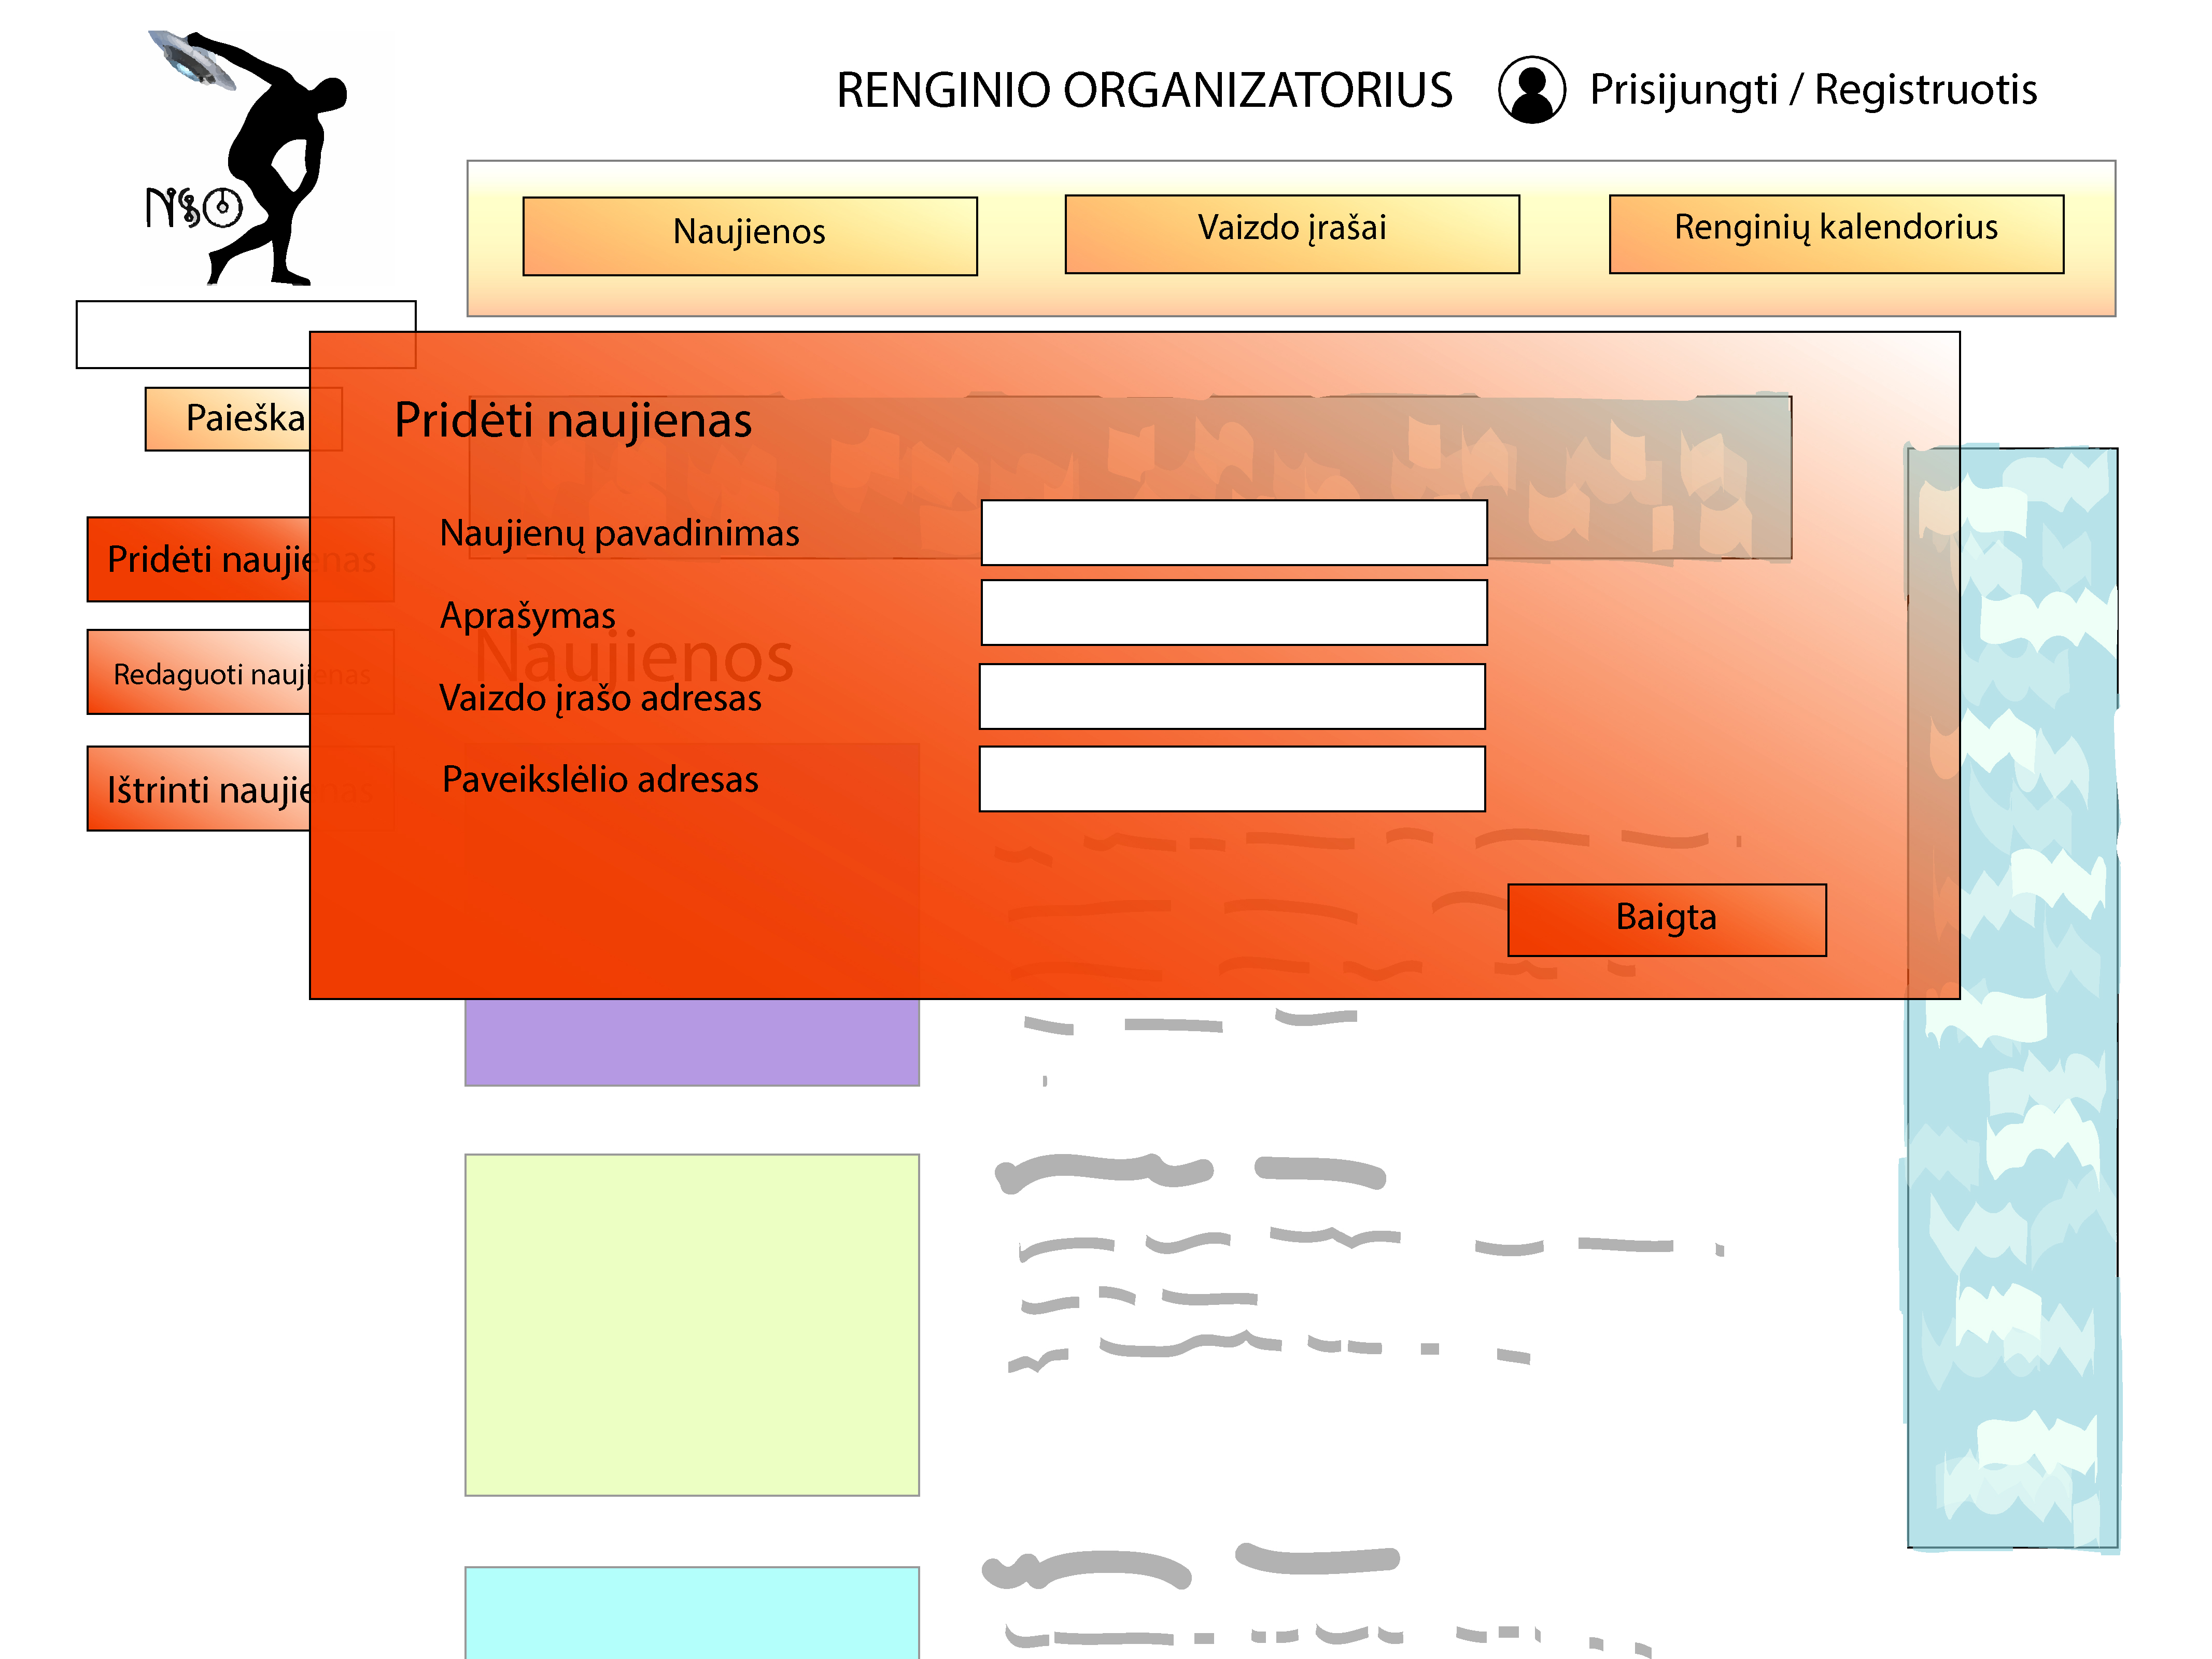
\includegraphics[width=\textwidth, height=8cm, keepaspectratio]{img/PSI4/OrganizatoriusNaujienos-01.jpg}
					\caption{Renginio organizatoriaus paskyra}
					\label{fig:uzd_org_pridetiNaujienas}
				\end{figure}
				
			\item \textbf{Redaguoti sukurtą naujieną}   \\
					Organizatorius paspaudžia ant naujienos kurią sukūrė, atsidarius naujienos puslapiui, paspaudžia mygtuką ,,Redaguoti''. Atsidaro naujienų redagavimo forma. Formos laukai yra užpildyti anksčiau įvesta informacija. Redagavus norimus laukus organizatorius paspaudžia ,,Išsaugoti''. Sistema atnaujina naujieną ir nukreipia į naujienos puslapį. 
					
					\underline{Alternatyvūs scenarijai:}
					\begin{itemize}
						\item Organizatorius nesuveda visų privalomų laukų. Jam neleidžia paspausti mygtuko ,,Išsaugoti'' ir prie atitinkamų laukų rašoma klaida.
					\end{itemize}	
				
			\item \textbf{Ištrinti sukurtą naujieną}   \\
					Organizatorius paspaudžia ant naujienos kurią sukūrė, atsidarius naujienos puslapiui, paspaudžia mygtuką ,,Ištrinti''. Sistema parodo patvirtinimo dialogą, organizatorius patvirtina ištrinimą, sistema panaikiną naujieną.
				
			\subsection* {Reikalavimų - užduočių atsekamumo matrica}
			\begin{table}[H]
				\centering
				\caption{Reikalavimų - užduočių atsekamumo matrica}
				\label{ReikalavimuUzduociuAtsekamumoMatrica}
				\begin{tabular}{|>
				{\columncolor[HTML]{9B9B9B}}l|l|l|l|l|l|l|l|l|l|l|l|l|l|l|l|l|l|l|l|l|l|} \hline
					X & \cellcolor[HTML]{D3D3D3}\rotatebox[origin=c]{90}{FR1} & \cellcolor[HTML]{9B9B9B}\rotatebox[origin=c]{90}{FR2} & 
					\cellcolor[HTML]{9B9B9B}\rotatebox[origin=c]{90}{FR3} & \cellcolor[HTML]{9B9B9B}\rotatebox[origin=c]{90}{FR4} & 
					\cellcolor[HTML]{9B9B9B}\rotatebox[origin=c]{90}{FR5} & \cellcolor[HTML]{9B9B9B}\rotatebox[origin=c]{90}{FR6} & 
					\cellcolor[HTML]{9B9B9B}\rotatebox[origin=c]{90}{FR7} & \cellcolor[HTML]{9B9B9B}\rotatebox[origin=c]{90}{FR8} & 
					\cellcolor[HTML]{9B9B9B}\rotatebox[origin=c]{90}{FR9} & \cellcolor[HTML]{9B9B9B}\rotatebox[origin=c]{90}{FR10} & 
					\cellcolor[HTML]{9B9B9B}\rotatebox[origin=c]{90}{FR11} & \cellcolor[HTML]{9B9B9B}\rotatebox[origin=c]{90}{FR12} &
					\cellcolor[HTML]{9B9B9B}\rotatebox[origin=c]{90}{FR13} & \cellcolor[HTML]{9B9B9B}\rotatebox[origin=c]{90}{FR14} & 
					\cellcolor[HTML]{9B9B9B}\rotatebox[origin=c]{90}{FR15} & \cellcolor[HTML]{9B9B9B}\rotatebox[origin=c]{90}{FR16} &
					\cellcolor[HTML]{9B9B9B}\rotatebox[origin=c]{90}{FR17} & \cellcolor[HTML]{9B9B9B}\rotatebox[origin=c]{90}{FR18} & 
					\cellcolor[HTML]{9B9B9B}\rotatebox[origin=c]{90}{FR19} & \cellcolor[HTML]{9B9B9B}\rotatebox[origin=c]{90}{FR20} & 
					\cellcolor[HTML]{9B9B9B}\rotatebox[origin=c]{90}{FR21}  \\ \hline
					U1  &      &      & X    &      &      &      &      &      &      &      &      &      &      &      &      &      &      &      &      &      &      \\ \hline
					U2  &      &      & X    &      &      &      &      &      &      &      &      &      &      &      &      &      &      &      &      &      &      \\ \hline
					U3  &      &      & X    &      &      &      &      &      &      &      &      &      &      &      &      &      &      &      &      &      &      \\ \hline
					U4  &      &      & X    &      &      &      &      &      &      &      &      &      &      &      &      &      &      &      &      &      &      \\ \hline
					U5  &      &      & X    &      &      &      &      &      &      &      &      &      &      &      &      &      &      &      &      &      &      \\ \hline
					U6  &      &      & X    &      &      &      &      &      &      &      &      &      &      &      &      &      &      &      &      &      &      \\ \hline
					U7  &      &      & X    &      &      &      &      &      &      &      &      &      &      &      &      &      &      &      &      &      &      \\ \hline
					U8  &      &      & X    &      &      &      &      &      &      &      &      &      &      &      &      &      &      &      &      &      &      \\ \hline
					U9  &      &      & X    &      &      &      &      &      &      &      &      &      &      &      &      &      &      &      &      &      &      \\ \hline
					U10 &      &      & X    &      &      &      &      &      &      &      &      &      &      &      &      &      &      &      &      &      &      \\ \hline
					U11 &      &      & X    &      &      &      &      &      &      &      &      &      &      &      &      &      &      &      &      &      &      \\ \hline
					U12 &      &      & X    &      &      &      &      &      &      &      &      &      &      &      &      &      &      &      &      &      &      \\ \hline
					U13 &      &      & X    &      &      &      &      &      &      &      &      &      &      &      &      &      &      &      &      &      &      \\ \hline
					U14 &      &      & X    &      &      &      &      &      &      &      &      &      &      &      &      &      &      &      &      &      &      \\ \hline
					U15 &      &      & X    &      &      &      &      &      &      &      &      &      &      &      &      &      &      &      &      &      &      \\ \hline
					U16 &      &      & X    &      &      &      &      &      &      &      &      &      &      &      &      &      &      &      &      &      &      \\ \hline 
					U17 &      &      & X    &      &      &      &      &      &      &      &      &      &      &      &      &      &      &      &      &      &      \\ \hline
					U18 &      &      & X    &      &      &      &      &      &      &      &      &      &      &      &      &      &      &      &      &      &      \\ \hline
					U19 &      &      & X    &      &      &      &      &      &      &      &      &      &      &      &      &      &      &      &      &      &      \\ \hline
					U20 &      &      & X    &      &      &      &      &      &      &      &      &      &      &      &      &      &      &      &      &      &      \\ \hline
					U21 &      &      & X    &      &      &      &      &      &      &      &      &      &      &      &      &      &      &      &      &      &      \\ \hline
					U22 &      &      & X    &      &      &      &      &      &      &      &      &      &      &      &      &      &      &      &      &      &      \\ \hline
					U23 &      &      & X    &      &      &      &      &      &      &      &      &      &      &      &      &      &      &      &      &      &      \\ \hline
					U24 &      &      & X    &      &      &      &      &      &      &      &      &      &      &      &      &      &      &      &      &      &      \\ \hline
					U25 &      &      & X    &      &      &      &      &      &      &      &      &      &      &      &      &      &      &      &      &      &      \\ \hline
					U26 &      &      & X    &      &      &      &      &      &      &      &      &      &      &      &      &      &      &      &      &      &      \\ \hline
					U27 &      &      & X    &      &      &      &      &      &      &      &      &      &      &      &      &      &      &      &      &      &      \\ \hline
					U28 &      &      & X    &      &      &      &      &      &      &      &      &      &      &      &      &      &      &      &      &      &      \\ \hline
					U29 &      &      & X    &      &      &      &      &      &      &      &      &      &      &      &      &      &      &      &      &      &      \\ \hline
					U30 &      &      & X    &      &      &      &      &      &      &      &      &      &      &      &      &      &      &      &      &      &      \\ \hline
					U31 &      &      & X    &      &      &      &      &      &      &      &      &      &      &      &      &      &      &      &      &      &      \\ \hline
					U32 &      &      & X    &      &      &      &      &      &      &      &      &      &      &      &      &      &      &      &      &      &      \\ \hline
					U33 &      &      & X    &      &      &      &      &      &      &      &      &      &      &      &      &      &      &      &      &      &      \\ \hline
					U34 &      &      & X    &      &      &      &      &      &      &      &      &      &      &      &      &      &      &      &      &      &      \\ \hline
				\end{tabular}
				\end{table}
			\begin{table}[H]
				\centering
				\begin{tabular}{|>
				{\columncolor[HTML]{9B9B9B}}l|l|l|l|l|l|l|l|l|l|l|l|l|l|l|l|l|l|l|l|l|l|} \hline
					X & \cellcolor[HTML]{D3D3D3}\rotatebox[origin=c]{90}{FR1} & \cellcolor[HTML]{9B9B9B}\rotatebox[origin=c]{90}{FR2} & 
					\cellcolor[HTML]{9B9B9B}\rotatebox[origin=c]{90}{FR3} & \cellcolor[HTML]{9B9B9B}\rotatebox[origin=c]{90}{FR4} & 
					\cellcolor[HTML]{9B9B9B}\rotatebox[origin=c]{90}{FR5} & \cellcolor[HTML]{9B9B9B}\rotatebox[origin=c]{90}{FR6} & 
					\cellcolor[HTML]{9B9B9B}\rotatebox[origin=c]{90}{FR7} & \cellcolor[HTML]{9B9B9B}\rotatebox[origin=c]{90}{FR8} & 
					\cellcolor[HTML]{9B9B9B}\rotatebox[origin=c]{90}{FR9} & \cellcolor[HTML]{9B9B9B}\rotatebox[origin=c]{90}{FR10} & 
					\cellcolor[HTML]{9B9B9B}\rotatebox[origin=c]{90}{FR11} & \cellcolor[HTML]{9B9B9B}\rotatebox[origin=c]{90}{FR12} &
					\cellcolor[HTML]{9B9B9B}\rotatebox[origin=c]{90}{FR13} & \cellcolor[HTML]{9B9B9B}\rotatebox[origin=c]{90}{FR14} & 
					\cellcolor[HTML]{9B9B9B}\rotatebox[origin=c]{90}{FR15} & \cellcolor[HTML]{9B9B9B}\rotatebox[origin=c]{90}{FR16} &
					\cellcolor[HTML]{9B9B9B}\rotatebox[origin=c]{90}{FR17} & \cellcolor[HTML]{9B9B9B}\rotatebox[origin=c]{90}{FR18} & 
					\cellcolor[HTML]{9B9B9B}\rotatebox[origin=c]{90}{FR19} & \cellcolor[HTML]{9B9B9B}\rotatebox[origin=c]{90}{FR20} & 
					\cellcolor[HTML]{9B9B9B}\rotatebox[origin=c]{90}{FR21}  \\ \hline
					U35 &      &      & X    &      &      &      &      &      &      &      &      &      &      &      &      &      &      &      &      &      &      \\ \hline
					U36 &      &      & X    &      &      &      &      &      &      &      &      &      &      &      &      &      &      &      &      &      &      \\ \hline
					U37 &      &      & X    &      &      &      &      &      &      &      &      &      &      &      &      &      &      &      &      &      &      \\ \hline
					U38 &      &      & X    &      &      &      &      &      &      &      &      &      &      &      &      &      &      &      &      &      &      \\ \hline
					U39 &      &      & X    &      &      &      &      &      &      &      &      &      &      &      &      &      &      &      &      &      &      \\ \hline
					U40 &      &      & X    &      &      &      &      &      &      &      &      &      &      &      &      &      &      &      &      &      &      \\ \hline
					U41 &      &      & X    &      &      &      &      &      &      &      &      &      &      &      &      &      &      &      &      &      &      \\ \hline
				\end{tabular}
			\end{table}
		\end{enumerate}
		
		
    \section{Peržiūros metu rastos klaidos}
		\begin{itemize}
			\item Dalykinės srities modelis suabstraktintas, nes iš pradžių buvo per daug lįsta į technines detales.
			\item FR2.4 Patikinti renginio organizatoriaus informaciją. ,,Patikinti'' pataisyta į ,,patikrinti''.
			\item Užduotis ,,Matyti privačius renginius''. Alternatyvus scenarijus, leidžiantis atfiltruoti tik privačius renginius perkeltas prie pagrindinio scenarijaus.
			\item Užduotis ,,Matyti privačius renginius''. Perrašyti alternatyvūs scenarijai.
			\item Neužsiregistravęs vartotojas pervadintas neprisijungusiu vartotoju.
			\item Pataisytos ir papildytos prisijungusio paprasto vartotojo užduotys.
			\item Pataisytos neprisijungusio vartotojo užduotys.Papildyti pagrindiniai ir alternatyvūs scenarijai.
			\item Sulietuvintos kabutės.
			\item Padalinta užduočių  diagrama į dvi diagramas.
			\item Ištaisytos gramatikos ir skyrybos klaidos.
			\item Renginio siūkymo formos mygtukas ,,Baigti'' pervadintas į ,,Siųsti''.
			\item Užduotyje U15 žodis ,,pasiektas'' pakeistas žodžiu ,,viršytas''.
		\end{itemize}
		
    \section{Priedai}\label{priedai}
        \subsection{Pradiniai užsakovo reikalavimai sistemai}
		\begin{enumerate}
			\item Internetinis puslapis turi būti pasiekiamas ir neprisijungusiems vartotojam.
			\item Neprisujungusiam vartotojui užėjus į puslapį, jam turi būti pateikiama tik neprisijungusiems vartotojams skirta informacija (t.y. naujienos, renginių kalendorius, vaizdo įrašai ir pan.)
			\item Būtina prisijungti norint pirkti bilietus, registruotis į renginį kaip dalyviui, aplikuoti į siūlomas darbo pozicijas.
			\item Kiekvienas vartotojas privalo turėti vartotojo vardą bei slaptažodį.
			\item Kiekvienas vartotojas gali anketoje suvesti papildomą asmeninę informaciją - vardą, pavardę, gimimo datą, telefono numerį, gyvenamąją vietą ir pan.
			\item Registruojantis į renginį ar aplikuojant į darbo pozicijas, vartotojo anketoje papildoma informacija yra privaloma.
			\item Registruojantis į komandinį renginį, reikia pasirinkti komandą, su kuria bus dalyvaujama. Jei komanda dar nesukurta, ją reikia sukurti registacijos metu anketoje.
			\item Registracijos metu anketoje kuriant komandą, reikia nurodyti komandos pavadinimą bei žmones, kurie bus komandos nariai.
			\item Pridėtiems komandos nariams yra išsiunčiami kvietimai, nariai gali juos priimti ar atmesti.
			\item Vaizdo įrašų numatytoji rikiavimo tvarka turi būti pagal datą, tačiau ją galima keisti (pvz. pagal peržiūras ar pan.)
			\item Rezultatų lentelės pateikiamos prie atitinkamo renginio.
			\item Dalyviai rezultatų lentelėje rikiuojami pagal jų rezultatą.
			\item Rezultatų lentelę galima filtruoti pagal kiekvieną atributą.
			\item Turi būti pateikiama sporto šakų, dalyvių bei komandų rezultatų istorija. Gali būti pateikiama tinkama statistika.
			\item Internetinėje svetainėje yra visiems prieinama sritis "Pateikti pasiūlymą", kurioje kiekvienas lankytojas gali pateikti pasiūlymą renginio organizatoriams.
			\item Pateikiant pasiūlymą reikia nurodyti savo elektroninį paštą (jei vartotojas prisijungęs - šis laukas užpildomas automatiškai) bei trumpą idėjos aprašą.
			\item Rėmėjų logotipai atvaizduojami internetiniame puslapyje tam skirtose vietose.
			\item Prisijungus kaip administratoriui, turi atsirasti prieiga prie administratoriaus skilties.
			\item Administratoriaus skiltyje turi būti galimybė peržiūrėti, pridėti, ištrinti bei atnaujinti naujienas, renginius, renginio rezultatus bei vaizdo įrašus vaizdo įrašus, apriboti ar blokuoti vartotojo prieigą, matyti visų dalyvių, renginių, aplikaciją pateikusių potencialių darbuotojų sąrašus.
			\item Prie kiekvieno renginio esančioje bilietų skiltyje, turi būti nurodomas bilietų likutis ir vieno bilieto kaina.
			\item Internetiniame puslapyje turi būti galimybė pasirinkti kitą kalbą iš lietuvių, anglų, rusų.
			\item Internetinis puslapis turi turėti savo analogą - mobiliąją programėlę. Visas funkcionalumas, esantis internetiniame puslapyje, turi būti ir mobiliojoje programėlėje. (Optional)
		\end{enumerate}
		
		\subsection{Užsakovo reikalavimų pakeitimai} 
			\begin{itemize}
				\item Visi reikalavimai susisteminti ir labiau klarifikuoti.
				\item 4 ir 5 reikalavimai sujungti į vieną.
				\item Dėl 2, 17, 19, 21 bei 22 reikalavimų buvo susisiekta su užsakovais. Pokalbiai pateikti žemiau.
				\item Reikalavimas numeris 17:
					\begin{itemize}
						\item \textit{Mes:} Sveiki, rašome jums iš UAB ,,Festofilas software group LT'', norime iš jūsų gauti patikslinimą dėl reikalavimo numeris 17. Norėtume tiksliau sužinoti vietas, kuriuose bus pateikti rėmėjų logotipai. Iš anksto ačiū.
						\item \textit{Užsakovas NR1:} ????
						\item \textit{Užsakovas NR1:} Su darbo vafovu
						\item \textit{Mes:} Ačiū už informaciją.
						\item[ ]
						\item \textit{Mes:} Sveiki, rašome jums iš UAB ,,Festofilas software group LT'', norime iš jūsų gauti patikslinimą dėl reikalavimo numeris 17. Norėtume tiksliau sužinoti vietas, kuriuose bus pateikti rėmėjų logotipai. Iš anksto ačiū.
						\item \textit{Užsakovas NR2:} Šias. 
\includegraphics{img/PSI4/smalllaugh.png}
						\item \textbf{Po 18 minučių}
						\item \textit{Užsakovas NR2:} Patikslinimas: Rėmėjų logotipams skirtos vietos yra: Puslapio viršuje, kairėje, dešinėje ir apačioje
						\item \textit{Užsakovas NR2:} :S
						\item \textit{Užsakovas NR2:} 
\includegraphics{img/PSI4/biglaugh.png}
						\item \textit{Mes:} Ačiū už informaciją.
					\end{itemize}	
				\item Reikalavimai numeris 21, 22:
					\begin{itemize}
						\item \textit{Mes:} Sveiki, rašome jums iš UAB ,,Festofilas software group LT'', norime pranešti, kad dėl laiko ir lėšų stokos mes turime atsisakyti, jūsų pateikto reikalavimo numeris 22, bei apriboti reikalavimą numeris 21 ties anglų kalba. Ar jums tinka?
						\item \textit{Užsakovas NR3:} Užsakovai nesupyks, jei atliksite viską vėluodami viena savaite!
						\item \textit{Mes:} Supratome, padarysime atsižvelgiant į esamus resursus.
						\item \textit{Užsakovas NR3:} Puiku, lauksime darbo pristatymo šį antradienį. Nors mūsų peržiūroje ir nebus.
					\end{itemize}
				\item Reikalavimai numeris 2, 19:
					\begin{itemize}
						\item \textit{Mes:} Sveiki, rašome jums iš UAB ,,Festofilas software group LT'', norime iš jūsų gauti patikslinimą dėl reikalavimų numeris 2 ir 19. Norėtume sužinoti kad bus vaizduojama naujienų skiltyje. Iš anksto ačiū.
						\item \textit{Užsakovas NR2:} :DDDDDDDDDDD
						\item \textit{Užsakovas NR2:} jūs dėl kiekvieno rašysit? 
\includegraphics{img/PSI4/smalllaugh.png}
						\item \textit{Mes:} Kolkas kituose reikalavimuose nematome diskutuotinų objektų, todėl nematome reikalo apie juos diskutuoti. Bet jei atsiras neaiškumų tai būtinai atsiklausime, norėdami užtikrinti mūsų paslaugų kokybę.
						\item \textit{Užsakovas NR2:} turėkit vaizduotės šiek tiek. 
\includegraphics{img/PSI4/wink.png}tai gali būti artėjantis koks nors įdomesnis renginys, praėjusio renginio rezultatai ir pan.
						\item \textit{Užsakovas NR2:} tai kad jau gal dėl 5 gavome žinučių. 
\includegraphics{img/PSI4/smile.png}
						\item \textit{Mes:} Primenu, kad išviso jūs pateikėte mums 22 reikalavimus
						\item \textit{Užsakovas NR2:} dėkoju už priminimą ir atsiprašau dėl nesklandumų. Tikiuosi daugiau jų nekils. Tačiau visada galite kreiptis.
						\item \textit{Mes:} Iškilo dar vienas klausimas: o kas ir kaip turėtų pateikti tas naujienas?
						\item \textit{Užsakovas NR2:} Organizatoriai pasirūpins jų įkėlimu. 
\includegraphics{img/PSI4/smile.png}
						\item \textit{Mes:} Supratome, dėkojame už greitus atsakymus.
						\item \textit{Užsakovas NR2:} Visada malonu bendradarbiauti. Pagarbiai „LtNSO,,
						\item[ ]
						\item \textit{Mes:} Sveiki, rašome jums iš UAB ,,Festofilas software group LT'', norime iš jūsų gauti patikslinimą dėl reikalavimų numeris 2 ir 19. Norėtume sužinoti kad bus vaizduojama naujienų skiltyje. Iš anksto ačiū.
						\item \textit{Užsakovas NR1:} Naujienos apie ateinancius ar buvusius renginiua
						\item \textit{Užsakovas NR1:} Arba tiesiogine "live" apzvalga is pacio renginio
						\item \textit{Mes:} Visvien neaiškų kas ir kaip turėtų pateikti tas naujienas.
						\item \textit{Užsakovas NR1:} Tai adminai arba organizatoriai renginio0
					\end{itemize}
			\end{itemize}
			
    \sectionnonum{Literatūros sąrašas} 
        \begin{itemize}
			\item Doc. dr. K. Petrausko Programų Sistemų Inžinerijos kurso konspektai
			\item Doc. dr. K. Petrausko Pirmojo laboratorinio darbo struktūra iš: http://www.mif.vu.lt/~karolis/PSI2.html
			\item A. Abran, J. W. Moore, P.Bourque, R. Dupuis, L. L. Tripp - ,,Guide to the Software Engineering Body of Knowledge''
			\item Latex dokumentacija: http://www.latex-project.org/help/documentation/
			\item D. Rosenberg, M. Stephens - ,,Use Case Driven Object Modeling with UML Theory and Practice''
        \end{itemize}
\end{document}
